%%%%%%%%%%%%%%%%%%%%%%%%%%%%%%%%%%%%%%%%%
% KOMA-Script Presentation
% LaTeX Template
% Version 1.1 (18/10/15)
%
% This template has been downloaded from:
% http://www.LaTeXTemplates.com
%
% Original Authors:
% Marius Hofert (marius.hofert@math.ethz.ch)
% Markus Kohm (komascript@gmx.info)
% Described in the PracTeX Journal, 2010, No. 2
%
% License:
% CC BY-NC-SA 3.0 (http://creativecommons.org/licenses/by-nc-sa/3.0/)
%
%%%%%%%%%%%%%%%%%%%%%%%%%%%%%%%%%%%%%%%%%

%----------------------------------------------------------------------------------------
%	PACKAGES AND OTHER DOCUMENT CONFIGURATIONS
%----------------------------------------------------------------------------------------
% KOMA-Script_MDPI_jpm-1309345
% compiling only on TexLive 2019

\documentclass[
paper=landscape,
paper=160mm:90mm, %128mm:96mm, % The same paper size as used in the beamer class
fontsize=11pt, % Font size
pagesize, % Write page size to dvi or pdf
parskip=half-, % Paragraphs separated by half a line
%captions=tableheading
]{scrartcl} % KOMA script (article)

\linespread{1.12} % Increase line spacing for readability



%~~~~~~~~~~~~~~~~~~~~~~~~~~~~~~~~~~~~~~~~~~~~~~~
% from main.tex
%%%%%%%%%%%%%%%%%%%%%%%%%%%%%%%%%% Tex
\maxdeadcycles=1000 % Output loop---200 consecutive dead cycles.

% http://mirror.ox.ac.uk/sites/ctan.org/macros/latex/contrib/biblatex/doc/biblatex.pdf it is compatible with KOMA-script
%\usepackage[backend=biber, style=authoryear, sorting=nyt, natbib=false]{biblatex}
% ****** backend=bibtex *******
\usepackage[backend=bibtex, style=authoryear]{biblatex}
%\bibliography{TCGA_margin_cutoff.bib, betel.bib, TMSB4X.bib, pvalueTex.bib}
% ~\autocite{}
\addbibresource{MRONJ.bib}
%\addbibresource{TCGA_margin_cutoff}
%\addbibresource{betel.bib}
%\addbibresource{TMSB4X.bib}
%\addbibresource{pvalueTex.bib}
%\addbibresource{Deep_Learning.bib}
% for citep
%\usepackage[comma,authoryear,square]{natbib} 
%\setcitestyle{authoryear,open={[},close={]}}
%\PassOptionsToPackage{comma,authoryear,square}{natbib}

\usepackage{wrapfig} % for wrapfigure, text wrapping figure
\newenvironment{WrapText1}[3][r]
{\wrapfigure[#2]{#1}{#3}}
{\endwrapfigure}
\newenvironment{WrapText2}[3][l]
{\wrapfigure[#2]{#1}{#3}}
{\endwrapfigure}
\newcommand{\wrapr}[6]{
\begin{minipage}{\linewidth}\mbox{}\\
\vspace{#1}
\begin{WrapText1}{#2}{#3}
\vspace{#4}#5\end{WrapText1}#6
\end{minipage}}

\newcommand{\wrapl}[6]{
\begin{minipage}{\linewidth}\mbox{}\\
\vspace{#1}
\begin{WrapText2}{#2}{#3}
\vspace{#4}#5\end{WrapText2}#6
\end{minipage}}

\usepackage{todonotes}

\usepackage{floatrow} % for side caption (beside)
%\floatsetup[widefigure]{margins=hangleft,capposition=beside,capbesideposition={center,outside},floatwidth=\textwidth} % {center,outside}
\usepackage{amsmath,amsfonts}
\usepackage{tikz-imagelabels} % for  tikz
\usepackage[bf]{caption}
\newcommand{\bcaption}[2]{\caption{\textbf{#1} #2}}

\usepackage{outlines}

\usepackage{pgfgantt} % for Gantt chart/flow chart
\definecolor{barblue}{RGB}{153,204,254}
\definecolor{groupblue}{RGB}{51,102,254}
\definecolor{linkred}{RGB}{165,0,33}

\usepackage{newfloat} % for caption of smartdiagram
\DeclareFloatingEnvironment[fileext=diag,placement={!ht},name=Figure ]{diag} % diag

\usepackage{smartdiagram} %flowchart
\usesmartdiagramlibrary{additions} 
\usepackage{tikz}   % for DAG plot by  tikzpicture
\usetikzlibrary{arrows}
% This is not an official TikZ library. Use at your own risk!
% https://tex.stackexchange.com/questions/5461/is-it-possible-to-change-the-size-of-an-arrowhead-in-tikz-pgf

\makeatletter
% alternative latex arrow
\pgfarrowsdeclare{latexnew}{latexnew}
{
  \ifdim\pgfgetarrowoptions{latexnew}=-1pt%
    \pgfutil@tempdima=0.28pt%
    \pgfutil@tempdimb=\pgflinewidth%
    \ifdim\pgfinnerlinewidth>0pt%
      \pgfmathsetlength\pgfutil@tempdimb{.6\pgflinewidth-.4*\pgfinnerlinewidth}%
    \fi%
    \advance\pgfutil@tempdima by.3\pgfutil@tempdimb%
  \else%
    \pgfutil@tempdima=\pgfgetarrowoptions{latexnew}%
    \divide\pgfutil@tempdima by 10%
  \fi%
  \pgfarrowsleftextend{+-1\pgfutil@tempdima}%
  \pgfarrowsrightextend{+9\pgfutil@tempdima}%
}
{
  \ifdim\pgfgetarrowoptions{latexnew}=-1pt%
    \pgfutil@tempdima=0.28pt%
    \pgfutil@tempdimb=\pgflinewidth%
    \ifdim\pgfinnerlinewidth>0pt%
      \pgfmathsetlength\pgfutil@tempdimb{.6\pgflinewidth-.4*\pgfinnerlinewidth}%
    \fi%
    \advance\pgfutil@tempdima by.3\pgfutil@tempdimb%
  \else%
    \pgfutil@tempdima=\pgfgetarrowoptions{latexnew}%
    \divide\pgfutil@tempdima by 10%
    \pgfsetlinewidth{0bp}%
  \fi%
  \pgfpathmoveto{\pgfqpoint{9\pgfutil@tempdima}{0pt}}
  \pgfpathcurveto
  {\pgfqpoint{6.3333\pgfutil@tempdima}{.5\pgfutil@tempdima}}
  {\pgfqpoint{2\pgfutil@tempdima}{2\pgfutil@tempdima}}
  {\pgfqpoint{-1\pgfutil@tempdima}{3.75\pgfutil@tempdima}}
  \pgfpathlineto{\pgfqpoint{-1\pgfutil@tempdima}{-3.75\pgfutil@tempdima}}
  \pgfpathcurveto
  {\pgfqpoint{2\pgfutil@tempdima}{-2\pgfutil@tempdima}}
  {\pgfqpoint{6.3333\pgfutil@tempdima}{-.5\pgfutil@tempdima}}
  {\pgfqpoint{9\pgfutil@tempdima}{0pt}}
  \pgfusepathqfill
}

% alternative latex reversed arrow
\pgfarrowsdeclarereversed{latexnew reversed}{latexnew reversed}{latexnew}{latexnew}

% alternative latex' arrow
\pgfarrowsdeclare{latex'new}{latex'new}
{
  \ifdim\pgfgetarrowoptions{latex'new}=-1pt%
    \pgfutil@tempdima=0.28pt%
    \advance\pgfutil@tempdima by.3\pgflinewidth%
  \else%
    \pgfutil@tempdima=\pgfgetarrowoptions{latex'new}%
    \divide\pgfutil@tempdima by 10%
  \fi%
  \pgfarrowsleftextend{+-4\pgfutil@tempdima}
  \pgfarrowsrightextend{+6\pgfutil@tempdima}
}
{
  \ifdim\pgfgetarrowoptions{latex'new}=-1pt%
    \pgfutil@tempdima=0.28pt%
    \advance\pgfutil@tempdima by.3\pgflinewidth%
  \else%
    \pgfutil@tempdima=\pgfgetarrowoptions{latex'new}%
    \divide\pgfutil@tempdima by 10%
    \pgfsetlinewidth{0bp}%
  \fi%
  \pgfpathmoveto{\pgfqpoint{6\pgfutil@tempdima}{0\pgfutil@tempdima}}
  \pgfpathcurveto
  {\pgfqpoint{3.5\pgfutil@tempdima}{.5\pgfutil@tempdima}}
  {\pgfqpoint{-1\pgfutil@tempdima}{1.5\pgfutil@tempdima}}
  {\pgfqpoint{-4\pgfutil@tempdima}{3.75\pgfutil@tempdima}}
  \pgfpathcurveto
  {\pgfqpoint{-1.5\pgfutil@tempdima}{1\pgfutil@tempdima}}
  {\pgfqpoint{-1.5\pgfutil@tempdima}{-1\pgfutil@tempdima}}
  {\pgfqpoint{-4\pgfutil@tempdima}{-3.75\pgfutil@tempdima}}
  \pgfpathcurveto
  {\pgfqpoint{-1\pgfutil@tempdima}{-1.5\pgfutil@tempdima}}
  {\pgfqpoint{3.5\pgfutil@tempdima}{-.5\pgfutil@tempdima}}
  {\pgfqpoint{6\pgfutil@tempdima}{0\pgfutil@tempdima}}
  \pgfusepathqfill
}

% alternative latex' reversed arrow
\pgfarrowsdeclarereversed{latex'new reversed}{latex'new reversed}{latex'new}{latex'new}

% alternative o arrow
\pgfarrowsdeclare{onew}{onew}
{
  \pgfarrowsleftextend{+-.5\pgflinewidth}
  \ifdim\pgfgetarrowoptions{onew}=-1pt%
    \pgfutil@tempdima=0.4pt%
    \advance\pgfutil@tempdima by.2\pgflinewidth%
    \pgfutil@tempdimb=9\pgfutil@tempdima\advance\pgfutil@tempdimb by.5\pgflinewidth%
    \pgfarrowsrightextend{+\pgfutil@tempdimb}%
  \else%
    \pgfutil@tempdima=\pgfgetarrowoptions{onew}%
    \advance\pgfutil@tempdima by -0.5\pgflinewidth%
    \pgfarrowsrightextend{+\pgfutil@tempdima}%
  \fi%
}
{ 
  \ifdim\pgfgetarrowoptions{onew}=-1pt%
    \pgfutil@tempdima=0.4pt%
    \advance\pgfutil@tempdima by.2\pgflinewidth%
    \pgfutil@tempdimb=0pt%
  \else%
    \pgfutil@tempdima=\pgfgetarrowoptions{onew}%
    \divide\pgfutil@tempdima by 9%
    \pgfutil@tempdimb=0.5\pgflinewidth%
  \fi%
  \pgfsetdash{}{+0pt}
  \pgfpathcircle{\pgfpointadd{\pgfqpoint{4.5\pgfutil@tempdima}{0bp}}%
                             {\pgfqpoint{-\pgfutil@tempdimb}{0bp}}}%
                {4.5\pgfutil@tempdima-\pgfutil@tempdimb}%
  \pgfusepathqstroke
}

% alternative square arrow
\pgfarrowsdeclare{squarenew}{squarenew}
{
 \ifdim\pgfgetarrowoptions{squarenew}=-1pt%
   \pgfutil@tempdima=0.4pt
   \advance\pgfutil@tempdima by.275\pgflinewidth%
   \pgfarrowsleftextend{+-\pgfutil@tempdima}
   \advance\pgfutil@tempdima by.5\pgflinewidth
   \pgfarrowsrightextend{+\pgfutil@tempdima}
 \else%
   \pgfutil@tempdima=\pgfgetarrowoptions{squarenew}%
   \divide\pgfutil@tempdima by 8%
   \pgfarrowsleftextend{+-7\pgfutil@tempdima}%
   \pgfarrowsrightextend{+1\pgfutil@tempdima}%
 \fi%
}
{
 \ifdim\pgfgetarrowoptions{squarenew}=-1pt%
   \pgfutil@tempdima=0.4pt%
   \advance\pgfutil@tempdima by.275\pgflinewidth%
   \pgfutil@tempdimb=0pt%
 \else%
   \pgfutil@tempdima=\pgfgetarrowoptions{squarenew}%   
   \divide\pgfutil@tempdima by 8%
   \pgfutil@tempdimb=0.5\pgflinewidth%
 \fi%
 \pgfsetdash{}{+0pt}
 \pgfsetroundjoin
 \pgfpathmoveto{\pgfpointadd{\pgfqpoint{1\pgfutil@tempdima}{4\pgfutil@tempdima}}
                            {\pgfqpoint{-\pgfutil@tempdimb}{-\pgfutil@tempdimb}}}
 \pgfpathlineto{\pgfpointadd{\pgfqpoint{-7\pgfutil@tempdima}{4\pgfutil@tempdima}}
                            {\pgfqpoint{\pgfutil@tempdimb}{-\pgfutil@tempdimb}}}
 \pgfpathlineto{\pgfpointadd{\pgfqpoint{-7\pgfutil@tempdima}{-4\pgfutil@tempdima}}
                            {\pgfqpoint{\pgfutil@tempdimb}{\pgfutil@tempdimb}}}
 \pgfpathlineto{\pgfpointadd{\pgfqpoint{1\pgfutil@tempdima}{-4\pgfutil@tempdima}}
                            {\pgfqpoint{-\pgfutil@tempdimb}{\pgfutil@tempdimb}}}
 \pgfpathclose
 \pgfusepathqfillstroke
}

% alternative stealth arrow
\pgfarrowsdeclare{stealthnew}{stealthnew}
{
  \ifdim\pgfgetarrowoptions{stealthnew}=-1pt%
    \pgfutil@tempdima=0.28pt%
    \pgfutil@tempdimb=\pgflinewidth%
    \ifdim\pgfinnerlinewidth>0pt%
      \pgfmathsetlength\pgfutil@tempdimb{.6\pgflinewidth-.4*\pgfinnerlinewidth}%
    \fi%
    \advance\pgfutil@tempdima by.3\pgfutil@tempdimb%
  \else%
    \pgfutil@tempdima=\pgfgetarrowoptions{stealthnew}%
    \divide\pgfutil@tempdima by 8%
  \fi%
  \pgfarrowsleftextend{+-3\pgfutil@tempdima}
  \pgfarrowsrightextend{+5\pgfutil@tempdima}
}
{
  \ifdim\pgfgetarrowoptions{stealthnew}=-1pt%
    \pgfutil@tempdima=0.28pt%
    \pgfutil@tempdimb=\pgflinewidth%
    \ifdim\pgfinnerlinewidth>0pt%
      \pgfmathsetlength\pgfutil@tempdimb{.6\pgflinewidth-.4*\pgfinnerlinewidth}%
    \fi%
    \advance\pgfutil@tempdima by.3\pgfutil@tempdimb%
  \else%
    \pgfutil@tempdima=\pgfgetarrowoptions{stealthnew}%
    \divide\pgfutil@tempdima by 8%
    \pgfsetlinewidth{0bp}%
  \fi%
  \pgfpathmoveto{\pgfqpoint{5\pgfutil@tempdima}{0pt}}
  \pgfpathlineto{\pgfqpoint{-3\pgfutil@tempdima}{4\pgfutil@tempdima}}
  \pgfpathlineto{\pgfpointorigin}
  \pgfpathlineto{\pgfqpoint{-3\pgfutil@tempdima}{-4\pgfutil@tempdima}}
  \pgfusepathqfill
}

% alternative stealth reversed arrow
\pgfarrowsdeclarereversed{stealthnew reversed}{stealthnew reversed}{stealthnew}{stealthnew}

% alternative to arrow
\pgfarrowsdeclare{tonew}{tonew}
{
  \ifdim\pgfgetarrowoptions{tonew}=-1pt%
    \pgfutil@tempdima=0.84pt%
    \advance\pgfutil@tempdima by1.3\pgflinewidth%
    \pgfutil@tempdimb=0.21pt%
    \advance\pgfutil@tempdimb by.625\pgflinewidth%
  \else%
    \pgfutil@tempdima=\pgfgetarrowoptions{tonew}%
    \pgfarrowsleftextend{+-0.8\pgfutil@tempdima}%
    \pgfarrowsrightextend{+0.2\pgfutil@tempdima}%
  \fi%
}
{
  \ifdim\pgfgetarrowoptions{tonew}=-1pt%
    \pgfutil@tempdima=0.28pt%
    \advance\pgfutil@tempdima by.3\pgflinewidth%
    \pgfutil@tempdimb=0pt,%
  \else%
    \pgfutil@tempdima=\pgfgetarrowoptions{tonew}%
    \multiply\pgfutil@tempdima by 100%
    \divide\pgfutil@tempdima by 375%
    \pgfutil@tempdimb=0.4\pgflinewidth%
  \fi%
  \pgfsetdash{}{+0pt}
  \pgfsetroundcap
  \pgfsetroundjoin
  \pgfpathmoveto{\pgfpointorigin}
  \pgflineto{\pgfpointadd{\pgfpoint{0.75\pgfutil@tempdima}{0bp}}
                         {\pgfqpoint{-2\pgfutil@tempdimb}{0bp}}}
  \pgfusepathqstroke
  \pgfsetlinewidth{0.8\pgflinewidth}
  \pgfpathmoveto{\pgfpointadd{\pgfqpoint{-3\pgfutil@tempdima}{4\pgfutil@tempdima}}
                             {\pgfqpoint{\pgfutil@tempdimb}{0bp}}}
  \pgfpathcurveto
  {\pgfpointadd{\pgfqpoint{-2.75\pgfutil@tempdima}{2.5\pgfutil@tempdima}}
               {\pgfqpoint{0.5\pgfutil@tempdimb}{0bp}}}
  {\pgfpointadd{\pgfqpoint{0pt}{0.25\pgfutil@tempdima}}
               {\pgfqpoint{-0.5\pgfutil@tempdimb}{0bp}}}
  {\pgfpointadd{\pgfqpoint{0.75\pgfutil@tempdima}{0pt}}
               {\pgfqpoint{-\pgfutil@tempdimb}{0bp}}}
  \pgfpathcurveto
  {\pgfpointadd{\pgfqpoint{0pt}{-0.25\pgfutil@tempdima}}
               {\pgfqpoint{-0.5\pgfutil@tempdimb}{0bp}}}
  {\pgfpointadd{\pgfqpoint{-2.75\pgfutil@tempdima}{-2.5\pgfutil@tempdima}}
               {\pgfqpoint{0.5\pgfutil@tempdimb}{0bp}}}
  {\pgfpointadd{\pgfqpoint{-3\pgfutil@tempdima}{-4\pgfutil@tempdima}}
               {\pgfqpoint{\pgfutil@tempdimb}{0bp}}}
  \pgfusepathqstroke
}

% alias alternative to arrow
\pgfarrowsdeclarealias{<new}{>new}{tonew}{tonew}

\makeatother

% tip length code
\pgfsetarrowoptions{latexnew}{-1pt}
\pgfsetarrowoptions{latex'new}{-1pt}
\pgfsetarrowoptions{onew}{-1pt}
\pgfsetarrowoptions{squarenew}{-1pt}
\pgfsetarrowoptions{stealthnew}{-1pt}
\pgfsetarrowoptions{tonew}{-1pt}
\pgfkeys{/tikz/.cd, arrowhead/.default=-1pt, arrowhead/.code={
  \pgfsetarrowoptions{latexnew}{#1},
  \pgfsetarrowoptions{latex'new}{#1},
  \pgfsetarrowoptions{onew}{#1},
  \pgfsetarrowoptions{squarenew}{#1},
  \pgfsetarrowoptions{stealthnew}{#1},
  \pgfsetarrowoptions{tonew}{#1},
}}

%\usepackage[]{caption} % bf
%\newcommand{\bcaption}[2]{\caption{\textbf{#1} #2}}
%\usepackage{outlines}
% mark in blue or red
%\usepackage{xcolor}

%\usepackage{xr-hyper}
%\usepackage{hyperref}
%\newcommand{\R}[1]{\label{#1}\linelabel{#1}} % for \label page and line
%\newcommand{\R}[1]{\linelabel{#1}} % for \label page and line
%\newcommand{\lr}[1]{page~\pageref{#1} (line~\lineref{#1})} % for \ref page and line
% for xr in your preamble
% https://www.overleaf.com/learn/how-to/Cross_referencing_with_the_xr_package_in_Overleaf
%\makeatletter
%\newcommand*{\addFileDependency}[1]{% argument=file name and extension
%  \typeout{(#1)}
%  \@addtofilelist{#1}
%  \IfFileExists{#1}{}{\typeout{No file #1.}}
%}
%\makeatother

%\newcommand*{\myexternaldocument}[1]{%
%    \externaldocument{#1}%
%    \addFileDependency{#1.tex}%
%    \addFileDependency{#1.aux}%
%}
% my external document I would like to reference the labels of. 
%\myexternaldocument{Supplementary_figures} %.tex .aux


%% not tikz
%\usepackage{pstricks-add}
%\usepackage{pst-all} % for PSTricks
%\usepackage{pst-plot,pst-eucl}
%\psset{algebraic,saveNodeCoors}

%\def\f{x+.5}
%\def\g{y-.5}% inverse of \f
%https://tex.stackexchange.com/questions/120788/draw-line-from-a-point-to-another-line-along-x-axis-or-y-axis-in-tikz/120817
%%
\usepackage{array}
\usepackage{ragged2e}
\usepackage{rotating}
\usepackage{tabularx} % for resizebox?
\usepackage{makecell}
% \usepackage{array}
\usepackage{multirow}
\usepackage{colortbl}     % arrayrulecolor
% \usepackage{colortbl}
\usepackage{longtable}

\usepackage{hhline}
%\usepackage{soul} % for \hl{}
\usepackage{siunitx} % for  1e-10 scientific notation, \num
%\usepackage{caption}
%\usepackage{subcaption}
%\usepackage{subcaption} % for figure  side by side, subfigure

%DIF 140a141
\usepackage{pbox} %DIF > 
%DIF -------

\usepackage{booktabs, multirow} % for borders and merged ranges
\usepackage{soul}% for underlines
%\usepackage[table]{xcolor} % for cell colors
\usepackage{changepage,threeparttable} 

%%% for abbreviations, or acronyms
\usepackage[acronym, nopostdot]{glossaries}  % automake
\usepackage{glossary-inline}
%\setacronymstyle{long-short}
%\renewcommand*{\glossarysection}[2][]{} 
%\renewcommand*{\glossarysection}[2][]{\textbf{#1}: }
% for abbreviations environment
%\newcommand{\abbrlabel}[1]{\makebox[3cm][l]{\textbf{#1}\ \dotfill}}
\newenvironment{abbreviation}


%\section{abbreviation}
%%%%%%%%%%%%% Define abbreviation
%\makeglossaries %https://tex.stackexchange.com/questions/110095/list-of-acronyms-is-not-displayed
\newacronym{hrv}{HRV}{heart rate variability}
\newacronym{ovh}{OVH}{oral verrucous hyperplasia}

\newacronym{tmuh}{TMUH}{Taipei Medical University Hospital}
\newacronym{tmu}{TMU}{Taipei Medical University}
\newacronym{tmwh}{TMWH}{Taipei Municipal Wan-Fang Hospital}

\newacronym{cnn}{CNN}{Convolutional Neural Network}
\newacronym{gnn}{GNN}{Graph Neural Network}
\newacronym{gcnn}{GCNN}{Graph Convolutional Neural Network}
\newacronym{rnn}{RNN}{Recurrent Neural Network}
\newacronym{ehr}{EHR}{electric healthcare records}


\newacronym{ptta}{PTTA}{p value of t-test or ANOVA}
\newacronym{anova}{ANOVA}{analysis of variance}
\newacronym{lcms}{LC-MS/MS}{liquid chromatography with tandem mass spectrometry}
\newacronym{maldi}{MALDI MS}{matrix-assisted laser desorption/ionization mass spectrometry}
\newacronym{maldii}{MALDI IMS}{matrix-assisted laser desorption/ionization imaging mass spectrometry}


\newacronym{ncbi}{NCBI}{National Center for Biotechnology Information}
\newacronym{degs}{DEGs}{differentially expressed genes}

\newacronym{ihc}{IHC}{immunohistochemistry}
\newacronym{fdr}{FDR}{false discovery rate}

\newacronym{hpa}{HPA}{the Human Protein Atlas}
\newacronym{hnscc}{HNSCC}{head and neck squamous cell carcinoma}
\newacronym{tcga}{TCGA}{the Cancer Genome Atlas}
\newacronym{tcpa}{TCPA}{the Cancer Proteome Atlas}
\newacronym{rna}{RNA}{ribonucleic acid}
\newacronym{rnaseq}{RNA-Seq}{RNA sequencing}
\newacronym{lncrna}{lncRNA}{long non-coding RNA}
%\newacronym{km}{KM}{Kaplan--Meier}
\newacronym{rppa}{RPPAs}{reverse-phase protein arrays}
\newacronym{rpma}{RPMA}{reverse-phase protein lysate microarray}

\newacronym{mmp}{MMP}{matrix metalloproteinase}
 %DKK1, CAMK2N1, STC2, PGK1, SURF4, USP10, NDFIP1, FOXA2, STIP1, and DKC1
 %ZNF557, ZNF266, IL19, MYO1H, FCGBP, LOC148709, EVPLL, PNMA5, KIAA1683, and NPB

\newacronym{DKK1}{DKK1}{dickkopf WNT signaling pathway inhibitor 1} 
\newacronym{CAMK2N1}{CAMK2N1}{calcium/calmodulin dependent protein kinase II inhibitor 1} 
\newacronym{CALML5}{CALML5}{calmodulin like 5}

\newacronym{STC2}{STC2}{stanniocalcin 2} 
\newacronym{PGK1}{PGK1}{phosphoglycerate kinase 1} 
\newacronym{SURF4}{SURF4}{surfeit 4} 
\newacronym{USP10}{USP10}{ubiquitin specific peptidase 10} 
\newacronym{NEDD4}{NEDD4}{neural precursor cell expressed, developmentally down-regulated 4}
\newacronym{NDFIP1}{NDFIP1}{NEDD4 family interacting protein 1} 
\newacronym{FOXA2}{FOXA2}{forkhead box A2} 
\newacronym{STIP1}{STIP1}{stress-induced-phosphoprotein 1} 
\newacronym{DKC1}{DKC1}{dyskeratosis congenita 1, dyskerin} 

\newacronym{ZNF557}{ZNF557}{zinc finger protein 557} 
\newacronym{ZNF266}{ZNF266}{zinc finger protein 266} 
\newacronym{IL19}{IL19}{interleukin 19} 
\newacronym{MYO1H}{MYO1H}{myosin 1H} 
\newacronym{FCGBP}{FCGBP}{Fc fragment of IgG binding protein} 
\newacronym{LOC148709}{LOC148709}{LncRNA LOC148709} 
\newacronym{EVPLL}{EVPLL}{envoplakin-like protein} 
\newacronym{PNMA5}{PNMA5}{paraneoplastic antigen like 5} 
%\newacronym{KIAA1683}{KIAA1683}{IQCN, IQ Motif Containing N} 
\newacronym{IQCN}{IQCN}{IQ motif containing N} % previous name KIAA1683
% "IQ'' refers to the first two amino acids of the motif: isoleucine (commonly) and glutamine (invariably)
\newacronym{NPB}{NPB}{neuropeptide B} 

 \newacronym{rt}{RT}{radiation therapy}
 \newacronym{nccn}{NCCN}{National Comprehensive Cancer Network}
 \newacronym{hif}{HIF}{hypoxia-inducible factor}
 \newacronym{egfr}{EGFR}{epidermal growth factor receptor}
 \newacronym{ras}{RAS}{rat sarcoma}
 \newacronym{hras}{HRAS}{Harvey rat sarcoma viral oncoprotein}
 \newacronym{erk}{ERK}{extracellular signal-regulated kinases}
 \newacronym{us}{US}{United States}
 \newacronym{fda}{FDA}{Food and Drug Administration}
 \newacronym{tpf}{Tax-PF}{docetaxel, cisplatin, and 5-fluorouracil}
 \newacronym{tki}{TKI}{tyrosine kinase inhibitor}
 \newacronym{her}{HER}{human epidermal growth factor receptor}
 \newacronym{ici}{ICI}{immune-checkpoint inhibitor}
 \newacronym{ctla4}{CTLA-4}{cytotoxic T lymphocyte antigen 4}
 \newacronym{pd1}{PD-1}{programmed death 1}
 \newacronym{pdl1}{PD-L1}{programmed death ligand 1}
 \newacronym{tim3}{TIM-3}{T-cell immunoglobulin mucin protein 3}
 \newacronym{lag3}{LAG-3}{lymphocyte activation gene 3}
 \newacronym{ifng}{IFN-$\gamma$}{interferon gamma}
 \newacronym{tigit}{TIGIT}{T cell immunoglobin and immunoreceptor tyrosine-based inhibitory motif}
 \newacronym{gitr}{GITR}{glucocorticoid-induced tumor necrosis factor receptor}
 \newacronym{vista}{VISTA}{V-domain Ig suppressor of T-cell activation}
 \newacronym{tmsb4x}{TMSB4X}{thymosin beta-4 X-linked}
 \newacronym{emt}{EMT}{epithelial-mesenchymal-transition}
 \newacronym{gdc}{GDC}{Genomic Data Commons}
 \newacronym{nci}{NCI}{the National Cancer Institute}
 \newacronym{gdac}{GDAC}{genome data analysis center}
 \newacronym{rest}{REST}{Representational State Transfer} 
 \newacronym{api}{API}{application programmable interface}
\newacronym{grch38}{GRCh38}{Genome Reference Consortium Homo sapiens genome assembly 38}
\newacronym{fpkm}{FPKM}{Fragments per kilobase per million reads mapped}
\newacronym{rsem}{RSEM}{RNA-Seq by Expectation-Maximization}
\newacronym{slca}{SLC35E2A}{solute carrier family 35 member E2A}
\newacronym{slcb}{SLC35E2B}{solute carrier family 35 member E2B}
\newacronym{cde}{CDE}{Common Data Element}
\newacronym{id}{ID}{identification}
\newacronym{ajcc}{AJCC}{the American Joint Committee on Cancer}
\newacronym{uicc}{UICC}{he Union for International Cancer Control}
\newacronym{tnm}{TNM}{the tumor size (T), cervical lymph node metastases (N), and distal metastasis status (M)}
\newacronym{ci95}{95\% CI}{95\% confidence interval}
\newacronym{os}{OS}{overall survival}
\newacronym{hr}{HR}{hazard ratio}
\newacronym{hpv}{HPV}{human papillomavirus}
\newacronym{ene}{ENE}{extra-nodal extension}
\newacronym{lvsi}{LVSI}{lymph-vascular space invasion}
\newacronym{pni}{PNI}{perineural invasion}
\newacronym{doi}{DOI}{depth of invasion}
\newacronym{lnd}{LND}{lymph node density}
\newacronym{wpoi5}{WPOI-5}{worst pattern of invasion score 5}
\newacronym{glut4}{GLUT4}{glucose transporter 4}
\newacronym{slc2a4}{SLC2A4}{solute carrier family 2 member A4}
\newacronym{trim24}{TRIM24}{tripartite motif-containing 24}
\newacronym{til}{TIL}{tumor-infiltrating lymphocytes}
\newacronym{tmb}{TMB}{tumor mutational burden}




%------------------------------------------------
\usepackage{outlines}
\usepackage[font={small}]{caption}
\newcommand{\bcaption}[2]{\caption{\textbf{#1} #2}}


\usepackage[margincaption]{sidecap}

\usepackage{subcaption} % for figure  side by side, subfigure

%%%%%% updated 2020 by esdd
%% https://tex.stackexchange.com/questions/547723/latex-throws-errors-on-section
%------------------------------------------------
% Colors
\usepackage[]{xcolor}  % table % Required for custom colors
% Define a few colors for making text stand out within the presentation
\definecolor{mygreen}{RGB}{44,85,17}
\definecolor{myblue}{RGB}{34,31,217}
\definecolor{mybrown}{RGB}{194,164,113}
\definecolor{myred}{RGB}{255,66,56}
% Use these colors within the presentation by enclosing text in the commands below

\newcommand*{\mygreen}[1]{\textcolor{mygreen}{#1}}
\newcommand*{\myblue}[1]{\textcolor{myblue}{#1}}
\newcommand*{\mybrown}[1]{\textcolor{mybrown}{#1}}
\newcommand*{\myred}[1]{\textcolor{myred}{#1}}

\definecolor{asparagus}{rgb}{0.53, 0.66, 0.42}

\newenvironment{MyColorPar}[1]{% for RED marked of revision
    \leavevmode\color{#1}\ignorespaces%
}{%
}%


% Margins
\usepackage[ % Page margins settings
  includeheadfoot,
  top=-1mm,
  bottom=1.5mm,
  left=1mm,
  right=3.5mm,
  headsep=0mm,
  footskip=8.5mm
]{geometry}

% Fonts
\usepackage[T1]{fontenc}     % For correct hyphenation and T1 encoding
\usepackage{lmodern} % Default font: latin modern font
%\usepackage{fourier} % Alternative font: utopia
%\usepackage{charter} % Alternative font: low-resolution roman font
\renewcommand{\familydefault}{\sfdefault} % Sans serif - this may need to be commented to see the alternative fonts

% Various required packages
\usepackage{amsthm} % Required for theorem environments
\usepackage{bm} % Required for bold math symbols (used in the footer of the slides)
\usepackage{tikz} % Required for colored boxes, loads graphicx and other packages
\usepackage{booktabs} % Required for horizontal rules in tables
\usepackage{multicol} % Required for creating multiple columns in slides
\usepackage{lastpage} % For printing the total number of pages at the bottom of each slide

\usepackage{microtype} % Better typography

% Slide layout configuration
\usepackage[automark]{scrlayer-scrpage} % Required for customization of the header and footer
\clearpairofpagestyles % Remove the default header and footer
\AddLayersAtBeginOfPageStyle{scrheadings}{headerbg,footerbg}% add background layers
\setkomafont{pageheadfoot}{\normalfont\sffamily} % Font settings for the header and footer
\setkomafont{pagehead}{\color{white}}
% Header configuration - if you don't want a header remove this block
\DeclareNewLayer[
  background,
  head,
  hoffset=0pt,
  width=\paperwidth,
  mode=picture,
  contents=\putLL{\myblue{\rule{\layerwidth}{\layerheight}}}
]{headerbg}

\ihead{\rightbotmark}

% Footer configuration
\KOMAoptions{footwidth=\textwidth+2mm:0pt}
\setkomafont{pagefoot}{\color{black}\tiny} % Small font size for the footnote
%\DeclareNewLayer[
  %background,
  %foot,
  %hoffset=0pt,
  %width=\paperwidth,
  %mode=picture,
  %contents=\putLL{\myblue{\rule{\layerwidth}{\layerheight}}}
%]{footerbg}
\ifoot{\runninghead~(OMS)\ \raisebox{0.2mm}{$\bm{\vert}$}\ \myuni} % Left side text
\ofoot*{\myauthor} % Right side;  %\myauthor\ % \pagemark/\pageref{LastPage}

% Sets vertical centering of slide contents with increased space between paragraphs/lists
\makeatletter
\renewcommand*{\@textbottom}{\vskip \z@ \@plus 1fil}
\newcommand*{\@texttop}{\vskip \z@ \@plus .5fil}
\setparsizes{1em}{\z@\@plus .25fil}{0pt plus 1fil}
\makeatother

% Remove page numbers and the dots leading to them from the outline slide
\DeclareTOCStyleEntries[linefill=\hfill,pagenumberbox=\gobble]{section}{section,subsection,subsubsection}
%\newcommand*\gobble[1]{}
\AfterTOCHead{\small}

%\renewcaptionname{english}{\contentsname}{Outline} % contentsname % Change the name of the table of contents
% Section spacing - deeper section titles are given less space due to lesser importance
\RedeclareSectionCommands[beforeskip=0pt,afterskip=0pt,afterindent=true,runin=false]{section,subsection,subsubsection}
\RedeclareSectionCommand[afterskip=-1mm]{subsection}
\RedeclareSectionCommand[afterskip=-2mm]{subsubsection}
\setcounter{secnumdepth}{\partnumdepth} % How deep sections are numbered

% Theorem style
\newtheoremstyle{mythmstyle} % Defines a new theorem style used in this template
  {0.5em} % Space above
  {0.5em} % Space below
  {} % Body font
  {} % Indent amount
  {\sffamily\bfseries} % Head font
  {} % Punctuation after head
  {\newline} % Space after head
  {\thmname{#1}\ \thmnote{(#3)}} % Head spec

\theoremstyle{mythmstyle} % Change the default style of the theorem to the one defined above
\newtheorem{theorem}{Theorem}[section] % Label for theorems
\newtheorem{remark}[theorem]{Remark} % Label for remarks
\newtheorem{algorithm}[theorem]{Algorithm} % Label for algorithms


% The code for the box which can be used to highlight an element of a slide (such as a theorem)
\newcommand*{\mybox}[2]{% The box takes two arguments: width and content
  \par\noindent
  \begin{tikzpicture}[mynodestyle/.style={rectangle,draw=myblue,thick,inner sep=2mm,text justified,top color=white,bottom color=white,above}]
    \node[mynodestyle,at={(0.5*#1+2mm+0.4pt,0)}]{% Box formatting
      \begin{minipage}[t]{#1}
      #2
      \end{minipage}%
    };
  \end{tikzpicture}
\par\vspace{-1.3em}}

%----------------------------------------------------------------------------------------
%	PRESENTER INFORMATION Tex Chi
%----------------------------------------------------------------------------------------
\usepackage{mfirstuc}
\MFUnocap{and}
\MFUnocap{for}
\MFUnocap{in}
\MFUnocap{at}
\MFUnocap{the}
% dissertation title: \title{\capitalisewords{global transcriptomics and proteomics analyses for biomarker identification and validation in head and neck squamous cell carcinoma}}
\newcommand*{\mytitle}{\capitalisewords{PGY Basic---Brief Introduction of Minor Oral Surgery}}
%English conversation at the Oral and Maxillofacial Surgery Clinic}}
%\newcommand*{\mytitle}{\capitalisewords{global transcriptomics and proteomics analyses for biomarker identification and validation in head and neck squamous cell carcinoma}}
%\newcommand*{\mytitle}{Global Proteomics-based Identification and Validation of Thymosin Beta-4 X-Linked as a Prognostic Marker for Head and Neck Squamous Cell Carcinoma} % old Title Transcriptomic Analysis for Prognostic Value in Head and Neck Squamous Cell Carcinoma
\newcommand*{\runninghead}{TMM} % Taiwan Medical Mission
%Deep Learning} % Running head displayed on almost all slides
\newcommand*{\myauthor}{Li-Hsing (Tex) Chi} % Presenters name(s)
\newcommand*{\myauthorWu}{Chia-Yu Wu}
\newcommand*{\myadvisorM}{Michael Hsiao}
\newcommand*{\myadvisorJ}{Yu-Chuan (Jack) Li}
\newcommand*{\myadvisorA}{Alexander TH Wu}
\newcommand*{\mydate}{2022/04/07} % \today Presentation date {2021/09/10} or {2021/12/10}
\newcommand*{\myuni}{Taipei Medical University} % University or department

\newcommand{\comm}[1]{} % for comment it out; https://tex.stackexchange.com/questions/17816/commenting-out-large-sections
%----------------------------------------------------------------------------------------
% for x \touchmarginincludegraphics
% for touch margins
% https://tex.stackexchange.com/questions/18166/how-to-have-a-figure-touch-the-edge-of-the-page
\newcommand{\mydimright}{%
  \dimexpr\paperwidth-1in-\hoffset-\oddsidemargin-
  \columnwidth-\columnsep\relax}
\newcommand{\mydimleft}{%
  \dimexpr1in+\hoffset+\oddsidemargin+\columnwidth\relax}

 

\begin{document}


%----------------------------------------------------------------------------------------
%	TITLE SLIDE
%----------------------------------------------------------------------------------------

% Title slide - you may have to tweak a few of the numbers if you wish to make changes to the layout
\thispagestyle{empty} % No slide header and footer
%\begin{figure}[!h]
% x \touchmarginincludegraphics[height=1cm]{TMWH2_logo}
%\end{figure}
\begin{tikzpicture}[remember picture, overlay]
    \node[anchor=north west, align=left, inner sep=13] at (current page.north west){
        
\includegraphics[width=8cm]{TMWH2_logo.png} \\};
\end{tikzpicture}
%
\includegraphics[width=8cm]{TMWH2_logo.png}
%{TMU_SOH_Logo.png} 6.5cm
%TMU_PTM_logo.png}
\begin{tikzpicture}[remember picture,overlay] % Background box
  \node [xshift=\paperwidth/2,yshift=\paperheight/2] at (current page.south west)
    [rectangle,fill,inner sep=0pt,minimum width=\paperwidth,minimum height=\paperheight/1.85,top color=myblue,bottom color=myblue]{}; % Change the height of the box, its colors and position on the page here
\end{tikzpicture}
% Text within the box
\begin{flushright}
%  \vspace{0.45cm}
  \color{white}\sffamily
  {\bfseries\Large\mytitle\par}% Title
  \vspace{0.2cm}
  \normalsize
%  \myauthorWu, DDS, Ph.D.  \hspace{10mm} \par 
 \underline{\myauthor}, DDS, Ph.D.  \hspace{10mm} \par % Author name
%  Advisors: \myadvisorM \hspace{1mm} \myadvisorJ\par \hspace{1mm} \myadvisorA\par

%  \myuni\par
%  \vfill
\end{flushright}
%Chi, L.-H., Wu, A. T. H., Hsiao, M. \& Li, Y.-C. (Jack). Journal of Personalized Medicine, 11, 782 (2021).
%\autocite{Chi2021}
%  \vspace{0.3cm}

\large \hspace{3cm} 
\textcolor{white}{$\longrightarrow$ 
Textbook: 
%"Dental Terminology" \footnotesize{(\url{shorturl.at/hoxN7})\\
Contemporary Oral and Maxillofacial Surgery (2019)}
}

% {shorturl.at/iqG18}
%A Holistic Way for Cancer Care
%\vspace{35mm}
\hspace{12cm}  \textcolor{white}{November 11, 2022}. %{\mydate} %\par % Date \today

\clearpage

%\begin{figure}
%    \centering
%    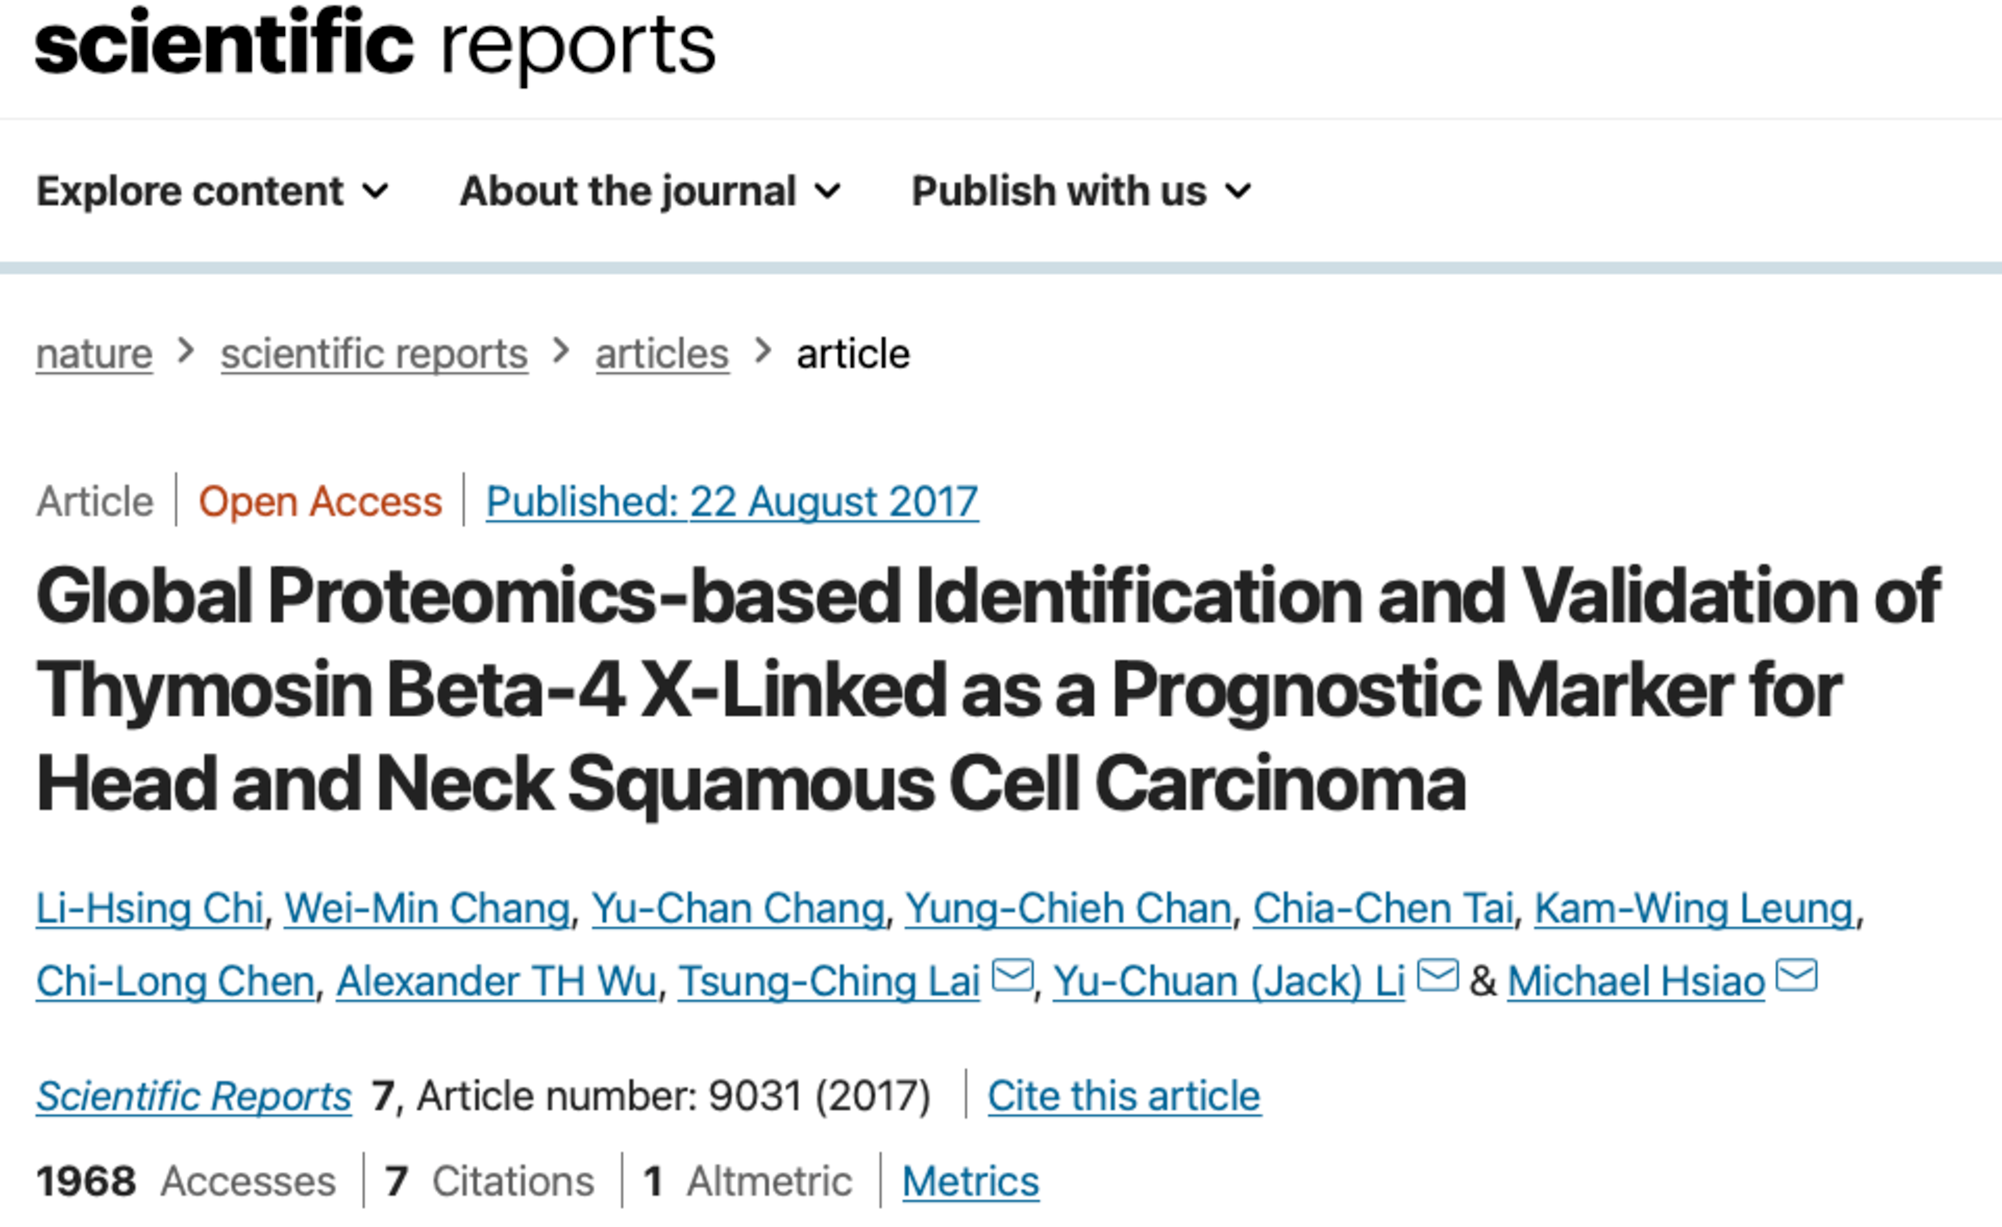
\includegraphics[width=13cm]{Article_Banner_TMSB4X_2017.pdf}
%    \caption{Caption}
%    \label{fig:my_label}
%\end{figure}
%\clearpage
%----------------------------------------------------------------------------------------
%	TABLE OF CONTENTS
%----------------------------------------------------------------------------------------

\thispagestyle{empty} % No slide header and footer

\small\tableofcontents % Change the font size and print the table of contents - it may be useful to shrink the font size further if the presentation is full of sections
% To exclude sections/subsections from the table of contents, put an asterisk after \(sub)section like so: \section*{Section Name}
%\clearpage

\comm{
\textbf{KEYWORD}\\
%head and neck squamous cell carcinoma (HNSCC);\\
%the Cancer Genome Atlas (TCGA); \\
\hl{transcriptomics};\hl{proteomics}; \\
\hl{RNA-seq}; \hl{mass spectrometry};\\
Cox's survival analysis; \hl{optimal cutoff} for Kaplan--Meier curve; \\
%effect size; hazard ratio in Cox's modeling;\\
%\acrfull{tmsb4x}; \\
%\acrfull{CALML5}; \\
%\acrfull{FCGBP}; \\
\hl{holistic cancer care}; mindfulness meditation.

} % end of comm
%\clearpage

%----------------------------------------------------------------------------------------
%	PRESENTATION SLIDES
%----------------------------------------------------------------------------------------

%\section*{Vize}

%\clearpage

%------------------------------------------------
%\pagestyle{plain}

\section{Tex Chi}
%中華民國口腔顎面外科專科醫師
%醫學資訊學碩士/中研院轉譯醫學博士
%中華民國駐非洲醫療團: 史瓦濟蘭(2009-2011)、聖多美(2011-2012),及史瓦濟蘭王室健檢團(2014-2018...); 索馬利蘭醫療團(2022-2023)
%臺灣法醫學會會員 (FORENSIC MEDICINE)
%門診戒菸服務醫師 (Tobacco quit)
%到宅牙醫服務(DOH)
%中西醫整合雷射針灸(laser acupuncture)
%全人照護 靈性關懷 (HOLISTIC CARE)

\begin{center}
    

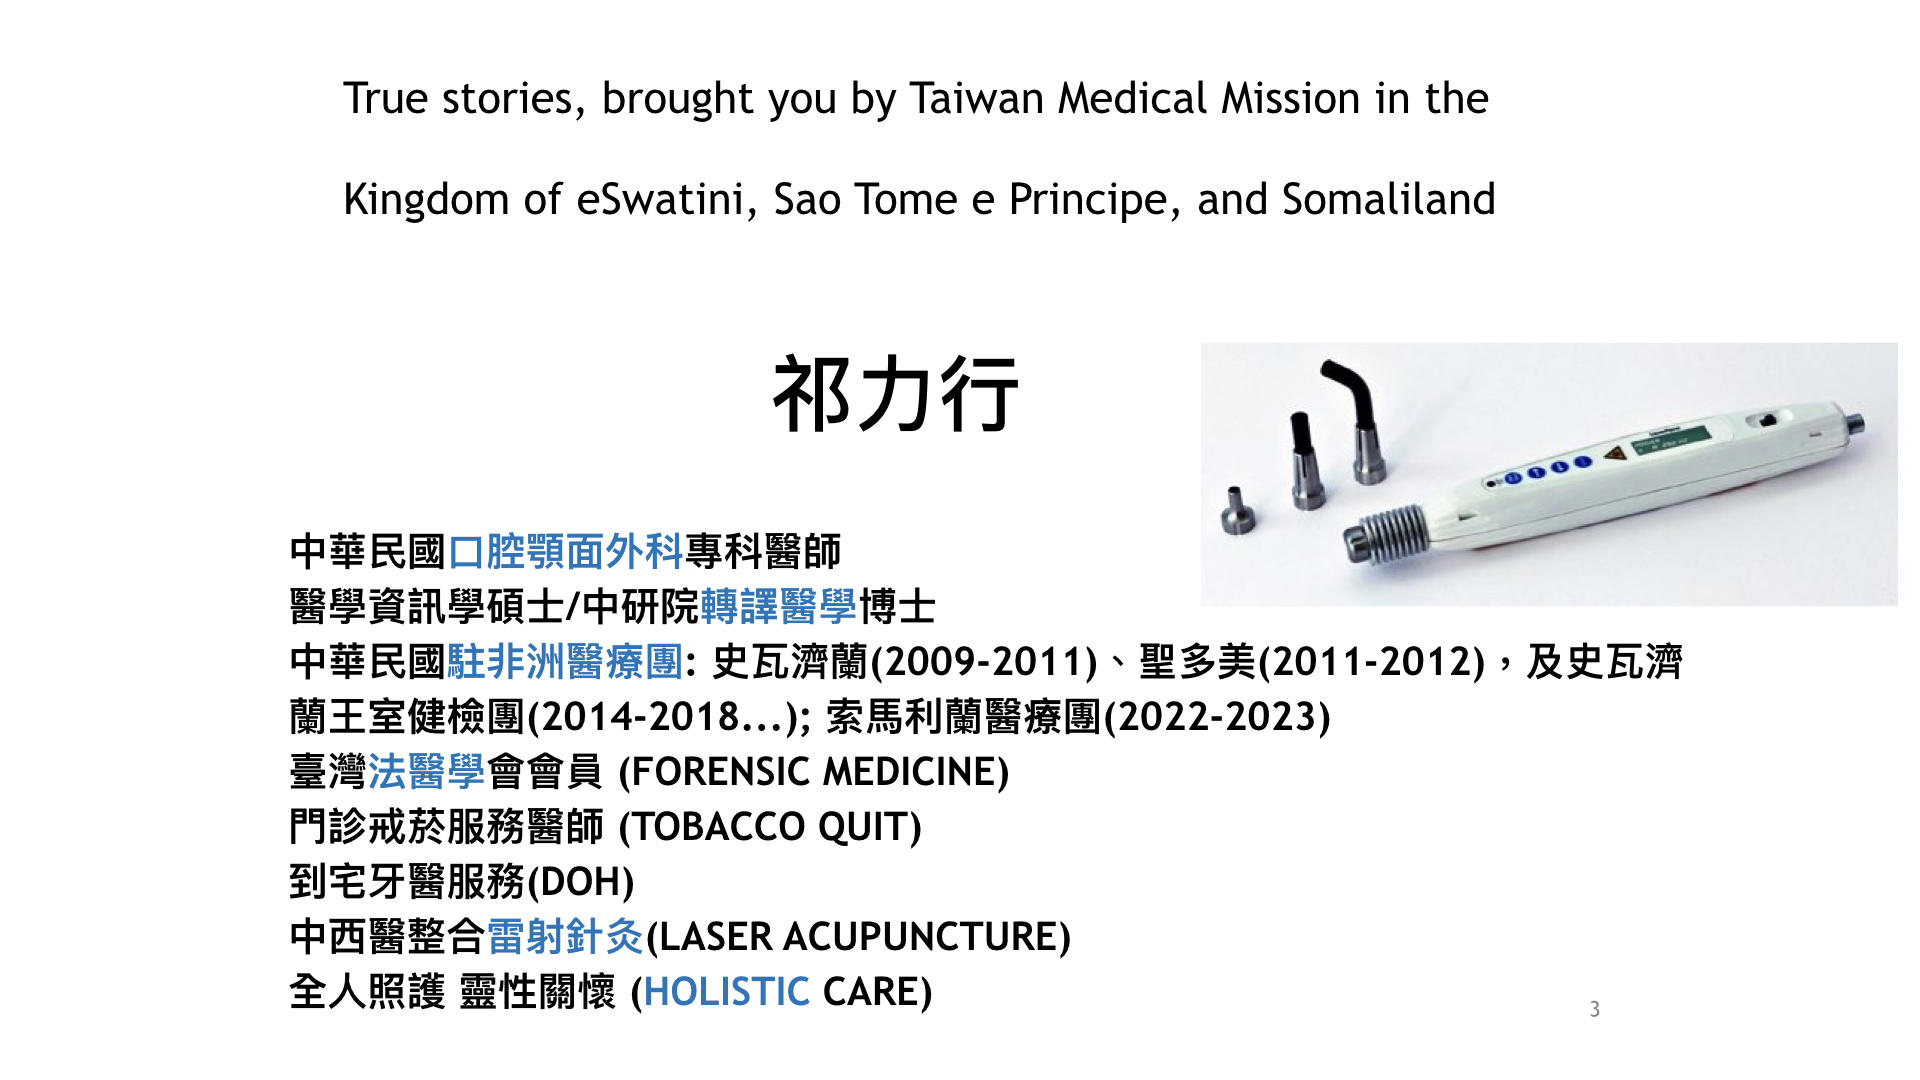
\includegraphics[width=0.85\linewidth]{ContemporaryOMS_Tex_CV.jpeg.001.jpeg}
%{TMU_IRP_Wu_workflow.png}
\end{center}


\section{Dentistry / dentistri /}

\begin{center}
    

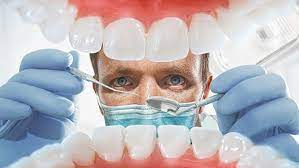
\includegraphics[width=11cm]{Dentistry.png}
%{TMU_IRP_Wu_workflow.png}
\end{center}

\section{Oral and Maxillofacial Surgery}

We, the oral and maxillofacial surgeons, are highly qualified professionals who research, diagnose, interview, treat, and care for patients suffering diseases of the head and neck.

\begin{tikzpicture}[remember picture,overlay] % Background box
  \node [xshift=\paperwidth/2,yshift=\paperheight/2.25] at (current page.south west)
    [rectangle,fill,inner sep=0pt,minimum width=\paperwidth,minimum height=\paperheight/2.35,top color=myblue,bottom color=myblue]{}; % Change the height of the box, its colors and position on the page here
\end{tikzpicture}


\includegraphics[width=13cm]{TAOMS_LOGO.png}

\clearpage
%% 
\section{Oral management strategies for radiotherapy of head and neck cancer} % 4
% reference: https://www.ncbi.nlm.nih.gov/pmc/articles/PMC7037635/

%\\
\begin{center} %[H]
    \centering
    \captionsetup{labelformat=empty}
    \captionof{table}{Let's go over vitals monitoring and treatment plan for a outpatient case:}
    % \captionabove{}
    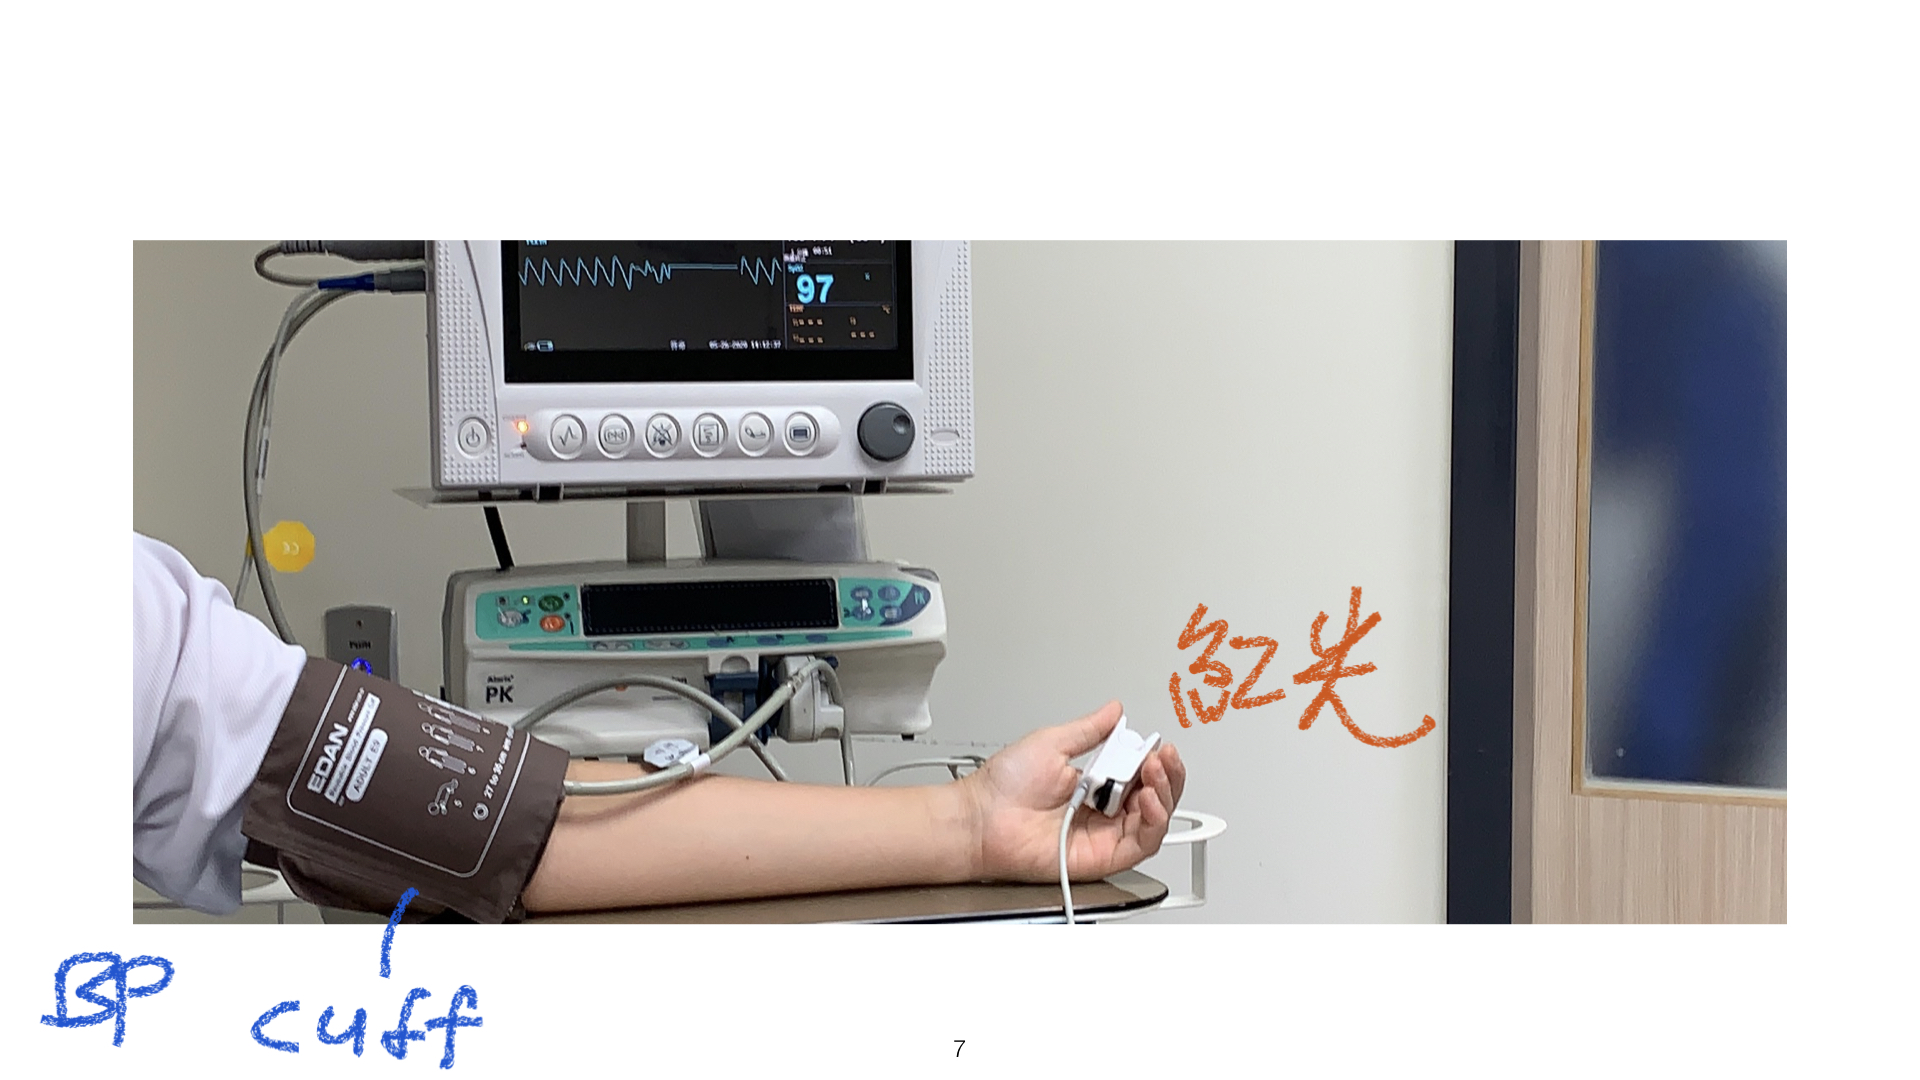
\includegraphics[width=9cm]{ContemporaryOMS_vitals.jpeg.001.jpeg}
\end{center}


%\clearpage


%\\
\begin{center} %[H]
    \centering
%    \captionsetup{labelformat=empty}
%    \captionof{table}{Let's go over vitals monitoring and treatment plan for a OPD case:}
    % \captionabove{}
    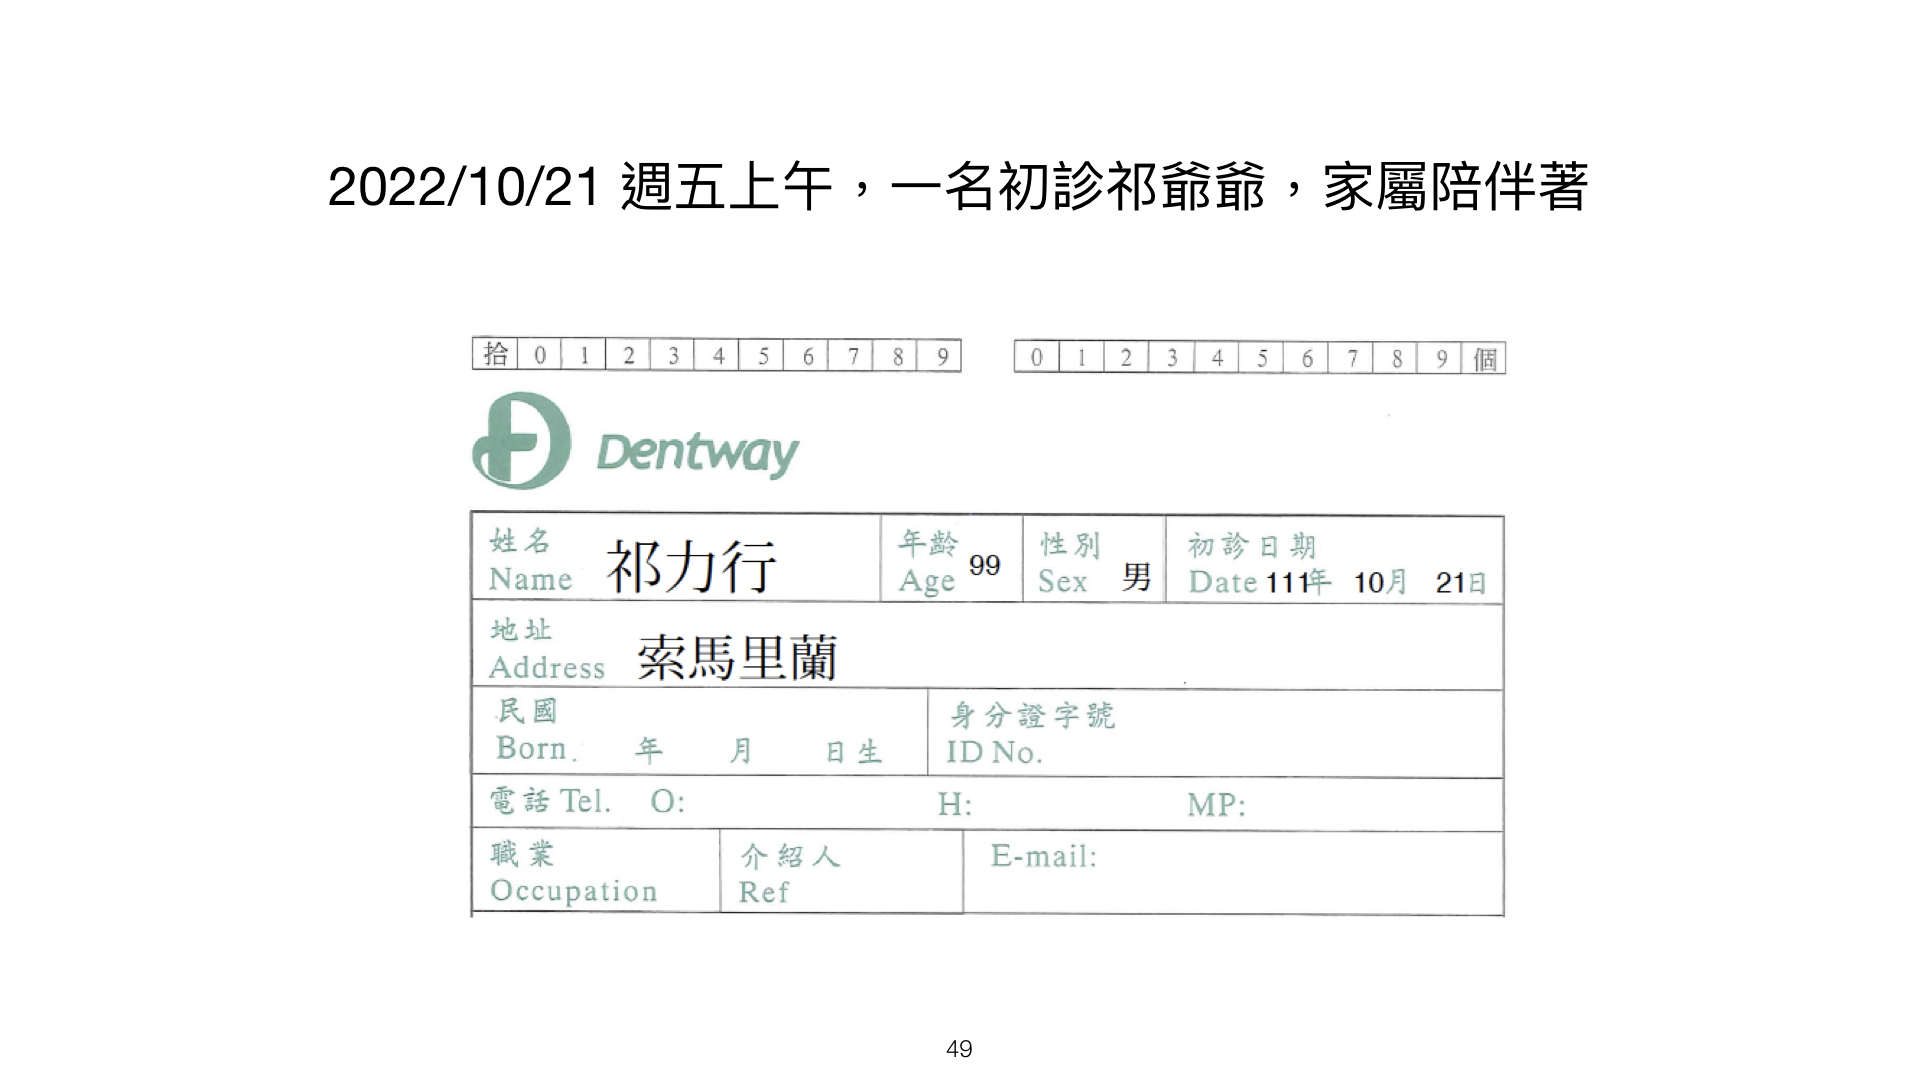
\includegraphics[width=11cm]{ContemporaryOMS_case祁爺爺.jpeg.001.jpeg}
    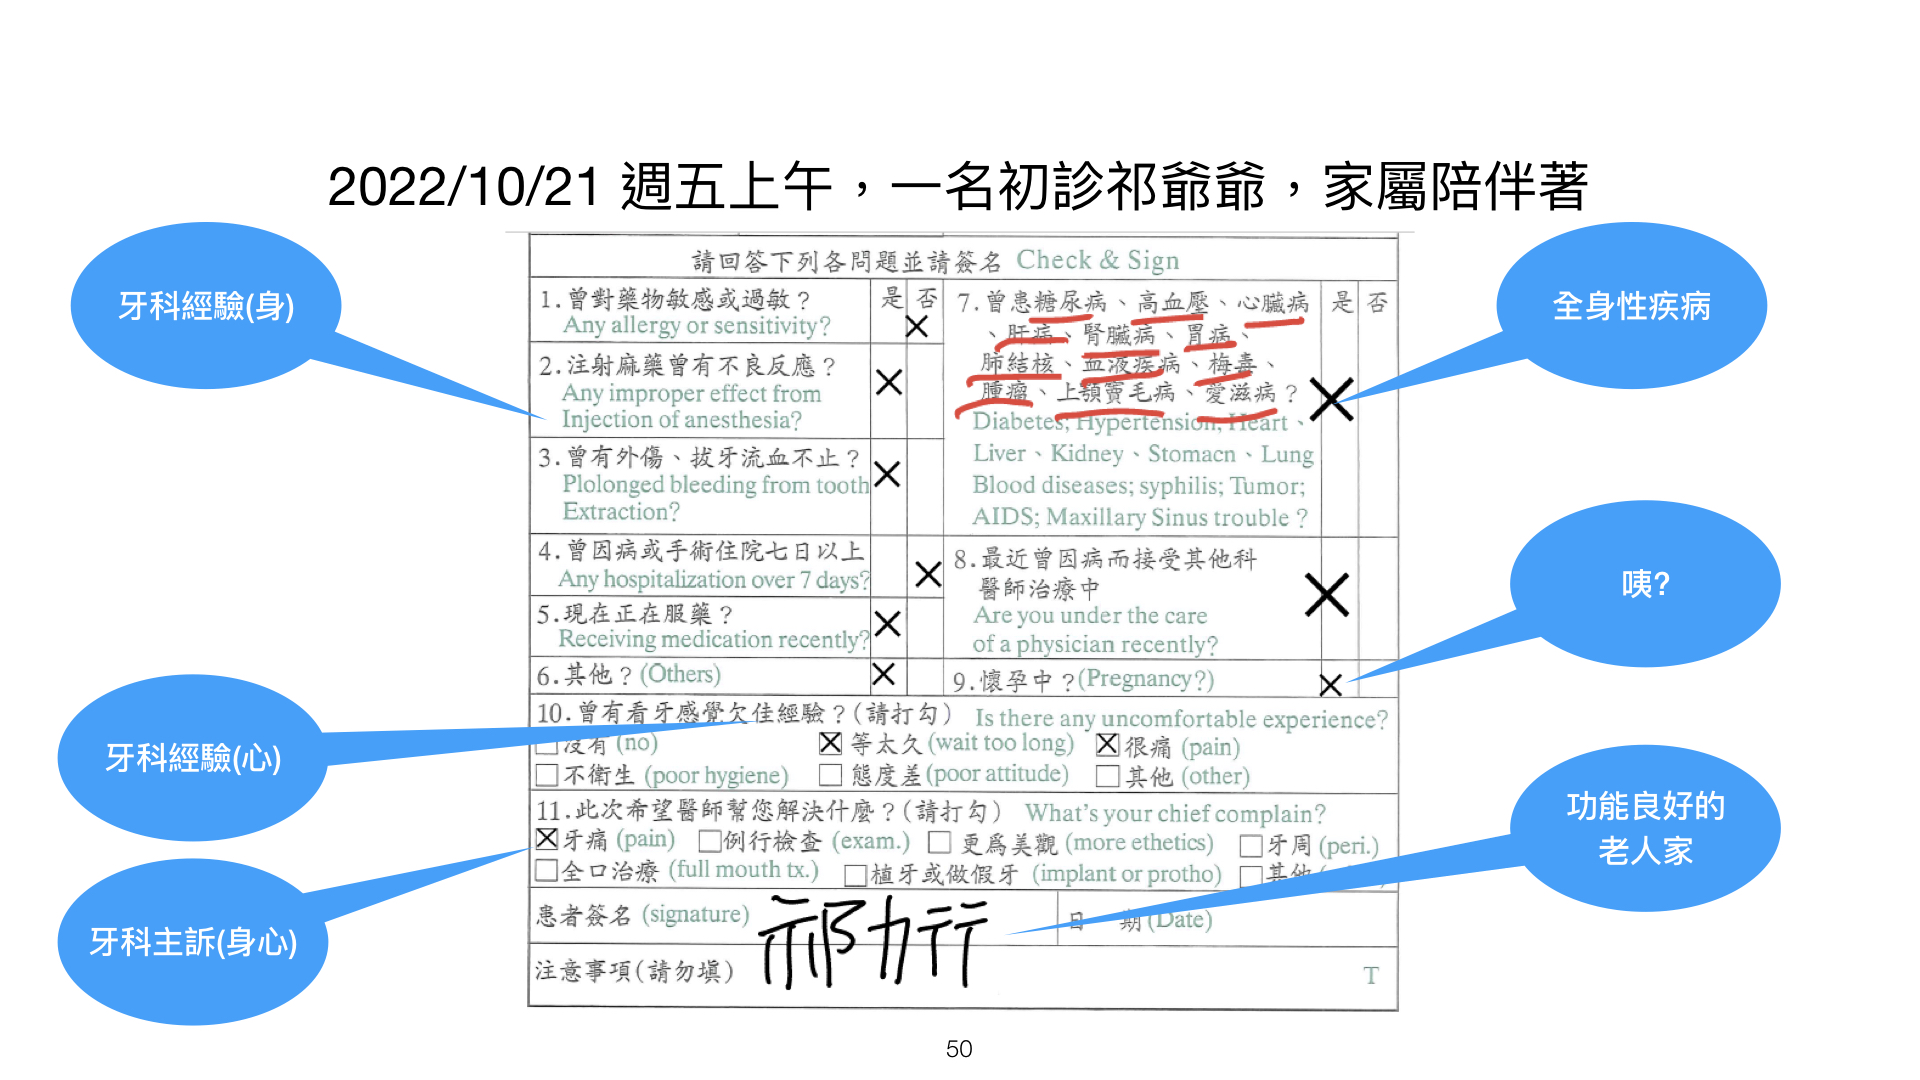
\includegraphics[width=12cm]{ContemporaryOMS_case祁爺爺.jpeg.002.jpeg}
    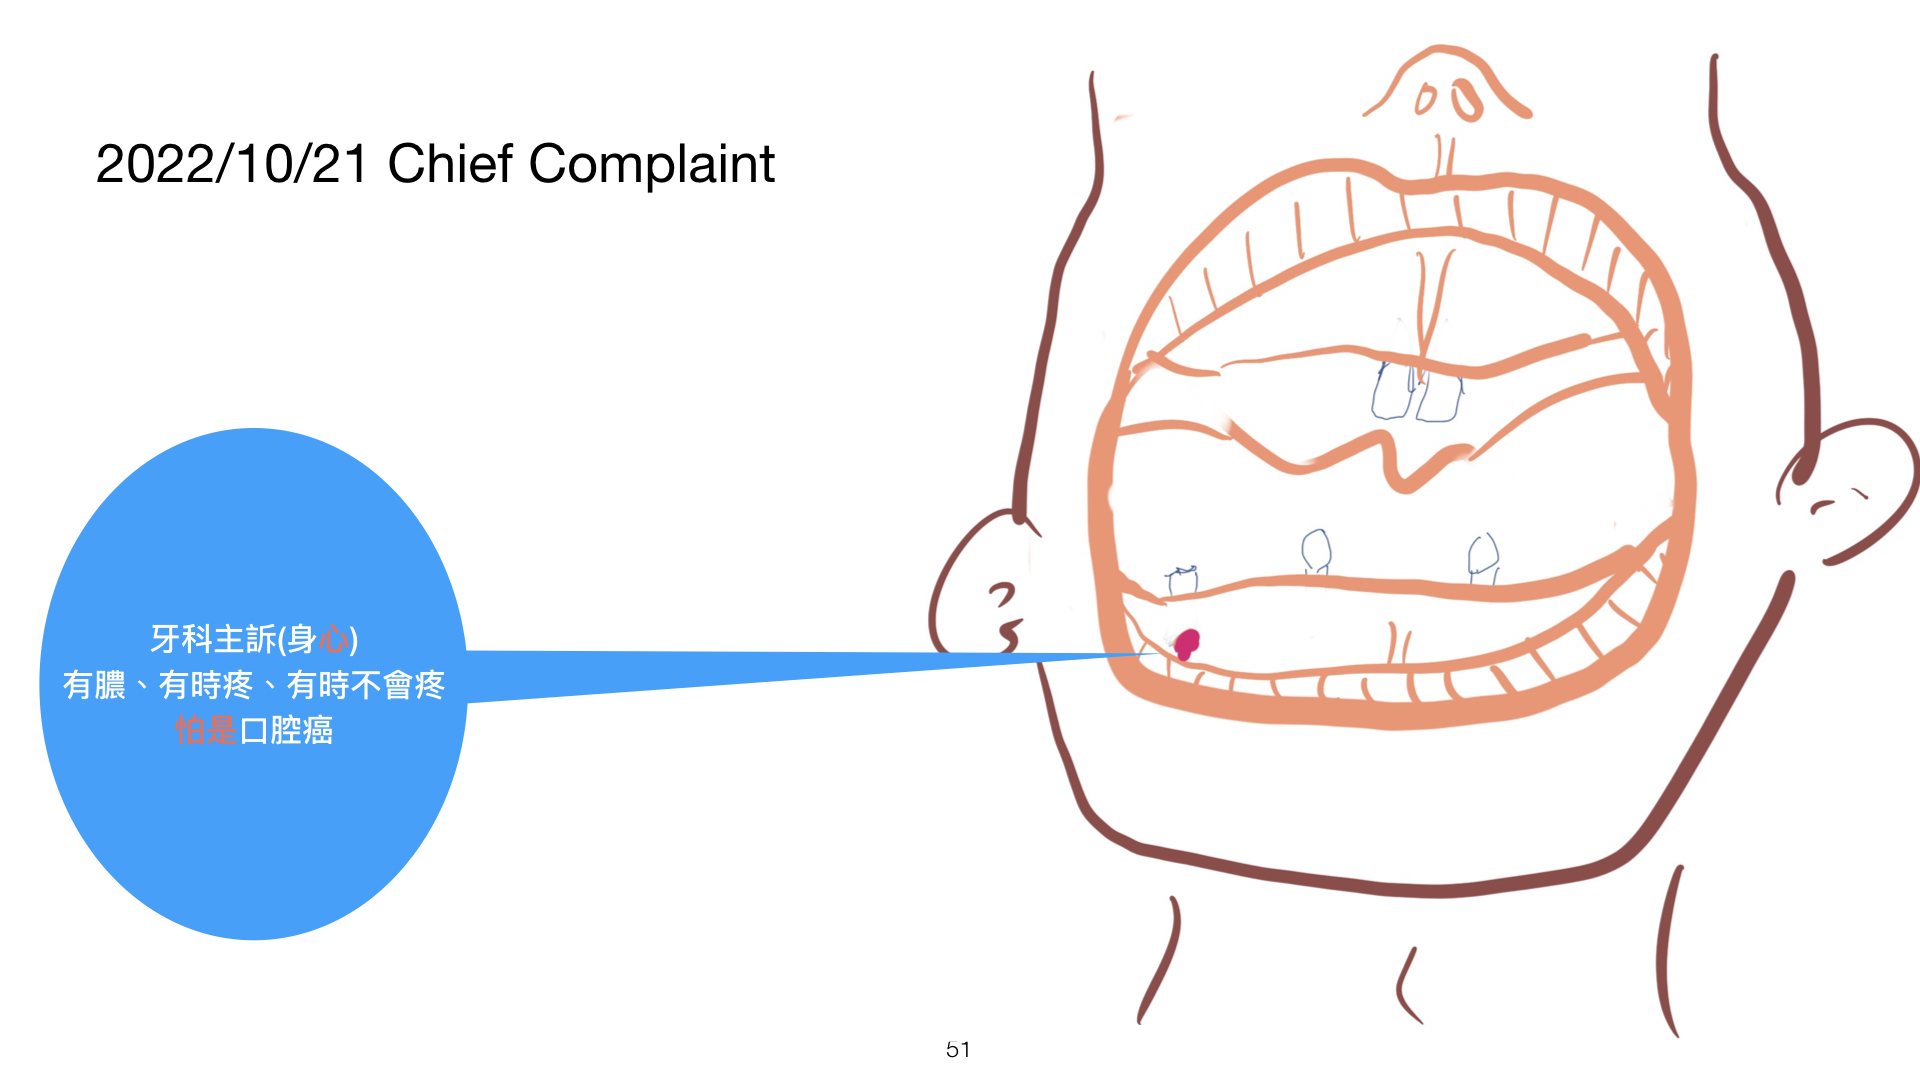
\includegraphics[width=12cm]{ContemporaryOMS_case祁爺爺.jpeg.003.jpeg}
    % informed consent form signed by Tex Chi
    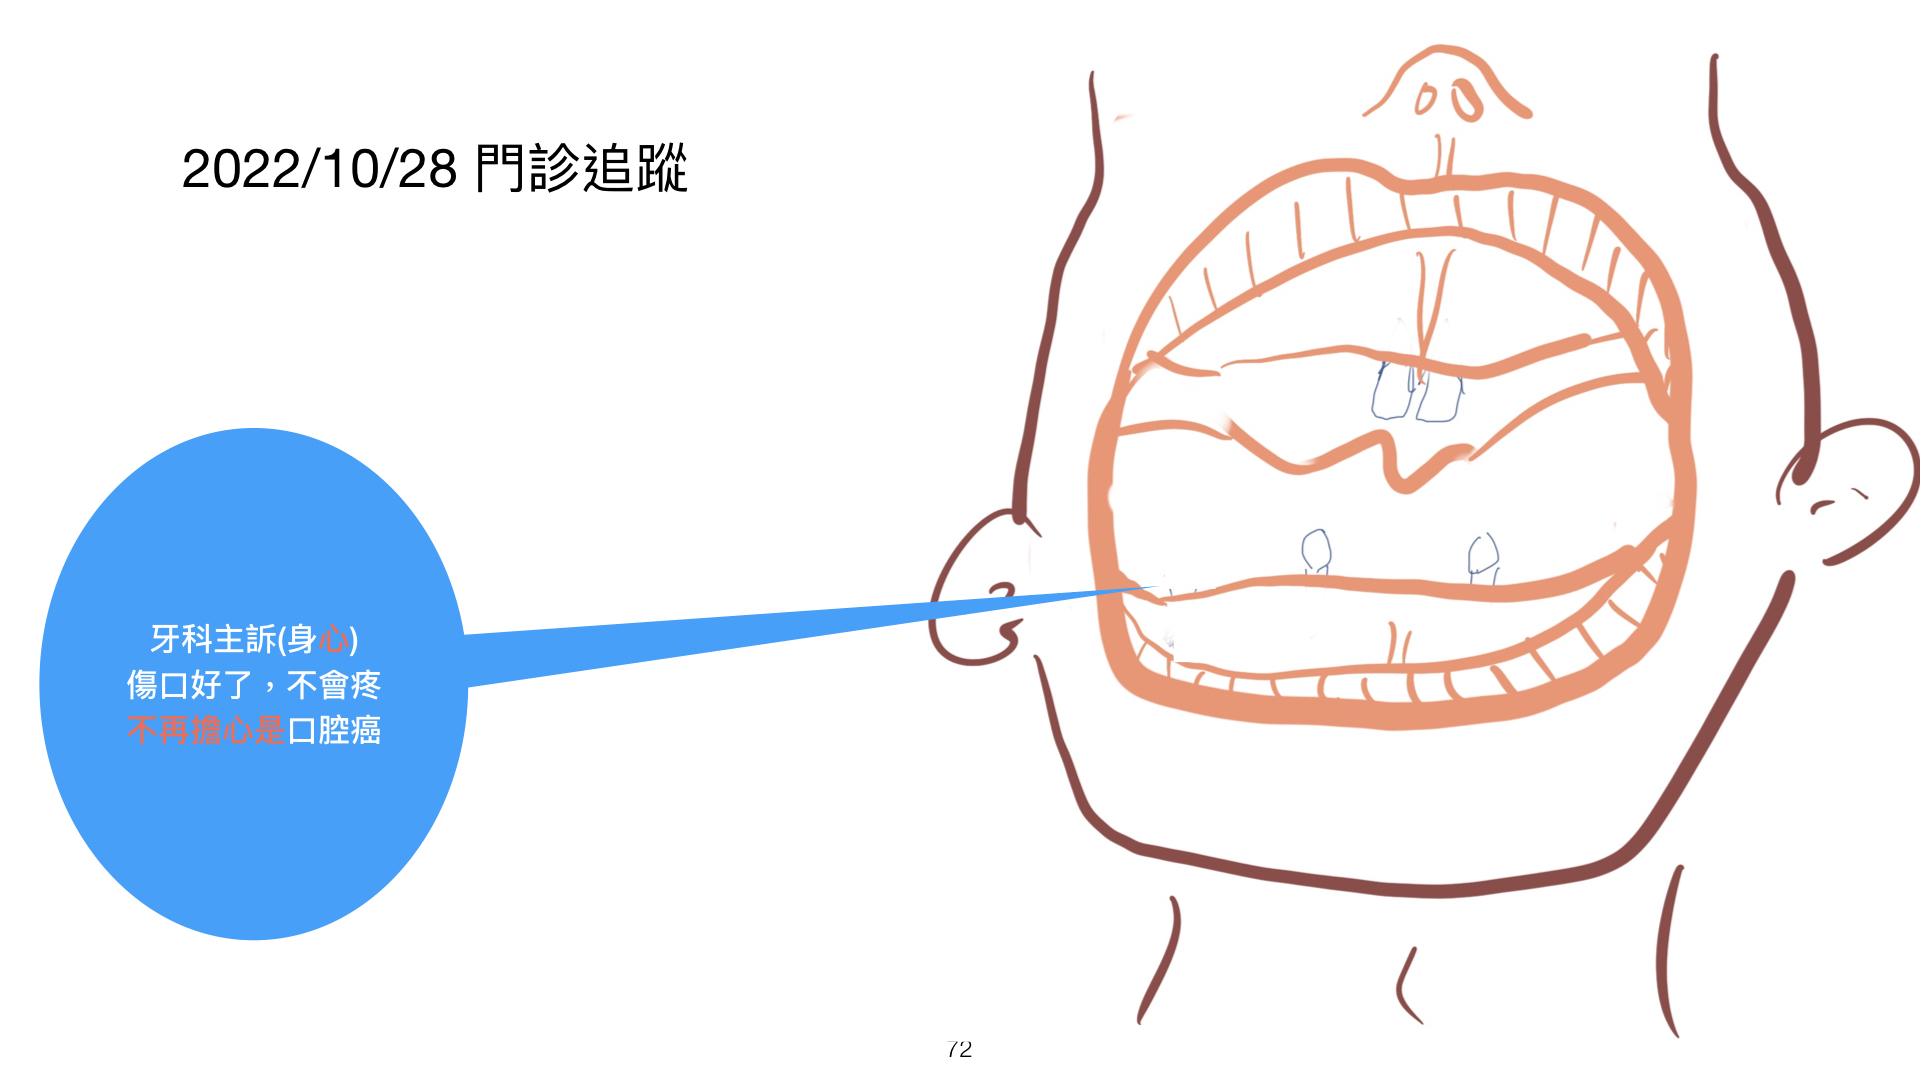
\includegraphics[width=12cm]{ContemporaryOMS_case祁爺爺.jpeg.004.jpeg}
        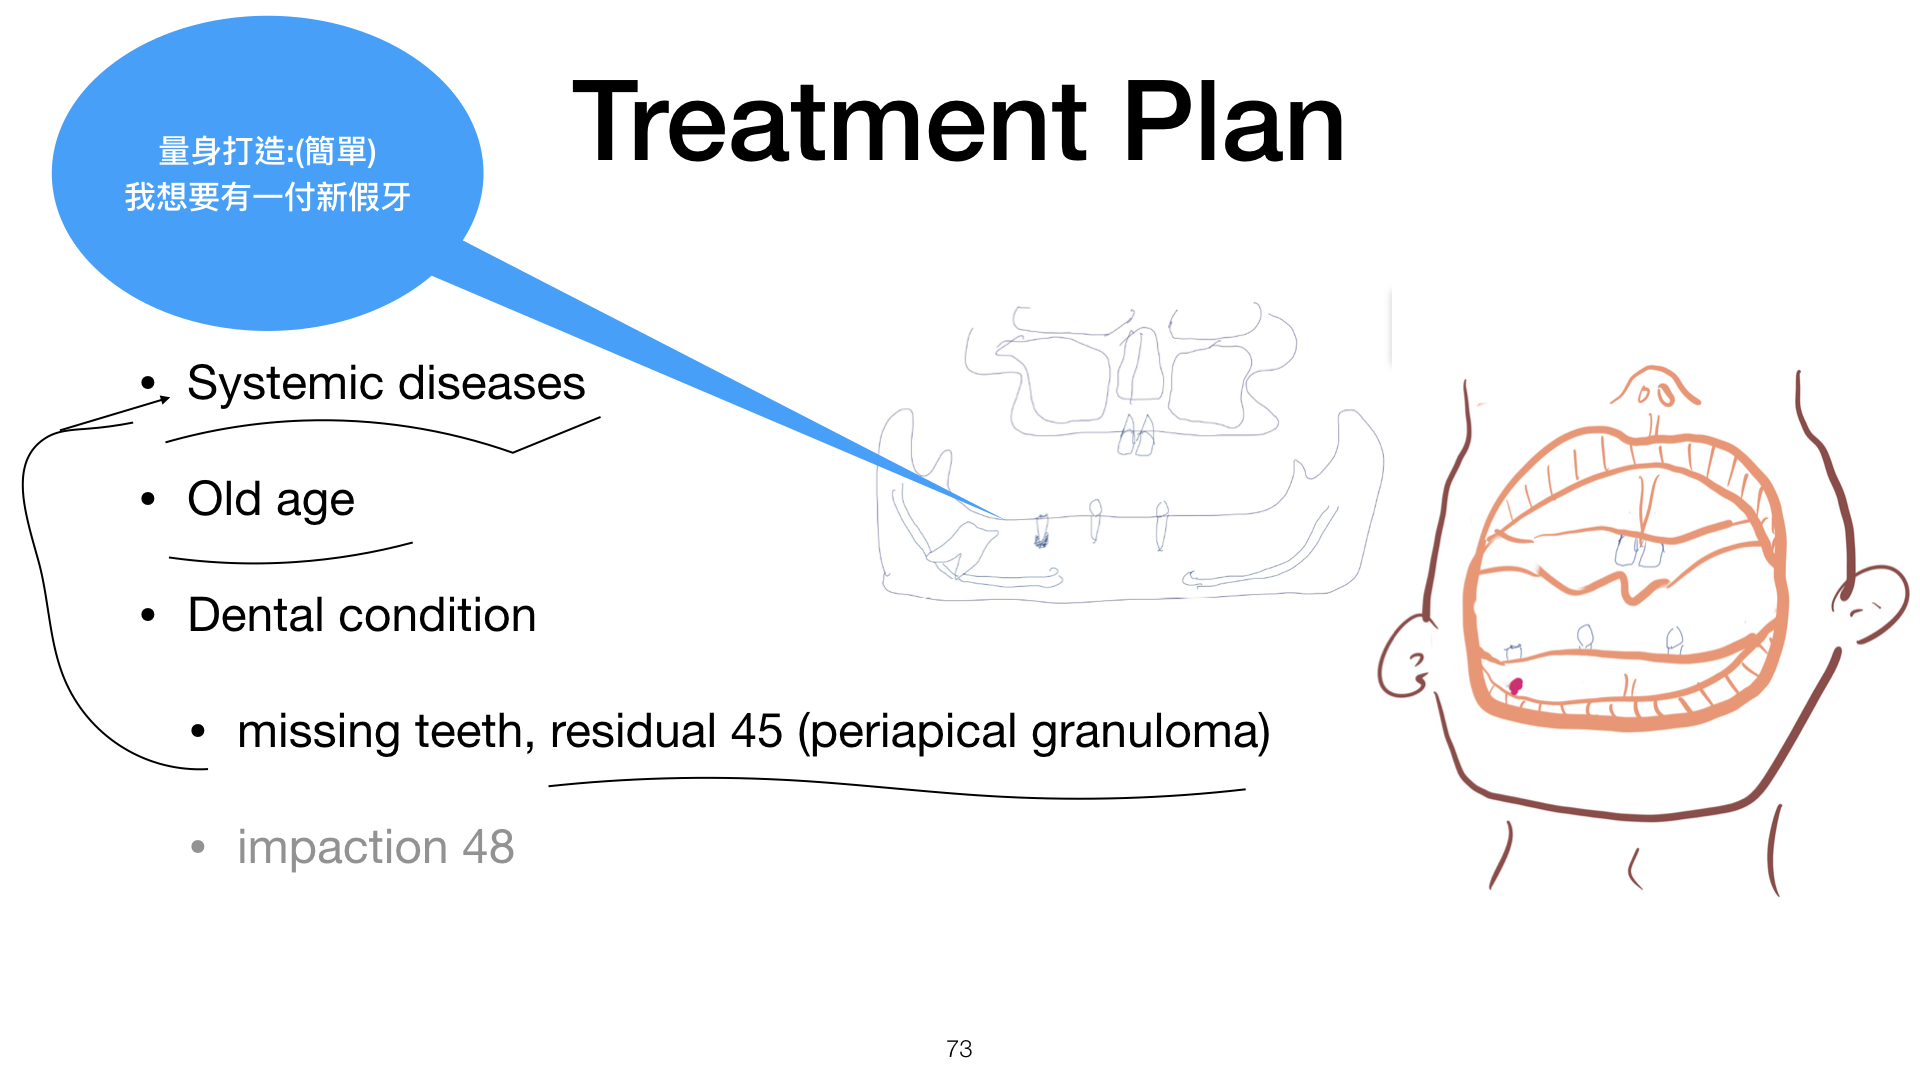
\includegraphics[width=12cm]{ContemporaryOMS_case祁爺爺.jpeg.005.jpeg}
\end{center}


%\clearpage

%%
\subsection{Prior to radiotherapy}
\subsubsection{Tooth extraction before the start of radiotherapy to prevent osteoradionecrosis}
%%
% - is up text, + is down image
\wrapr{-1mm}{7}{9cm}{-15mm}
{% figure
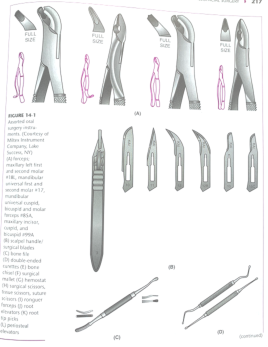
\includegraphics[width=5.5cm]{p217.pdf}
%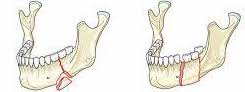
\includegraphics[width=5.5cm]{reduction_mandible.jpeg}
} % end of figure
{% text
\begin{outline}
\0 (phonetic spelling)
\1 forceps (FOUR-seps)
\1 scalpel handle and scalpel (SKAL-pel)
\1 bone file
\1 curette (cu-RET)
\end{outline}
} % end of text
%%
\clearpage

\subsubsection{Preparation of spacers to prevent serious oral mucositis}
% from comtemporary OMS textbook
%%
% - is up text, + is down image
\wrapr{-1mm}{7}{9cm}{-10mm}
{% figure
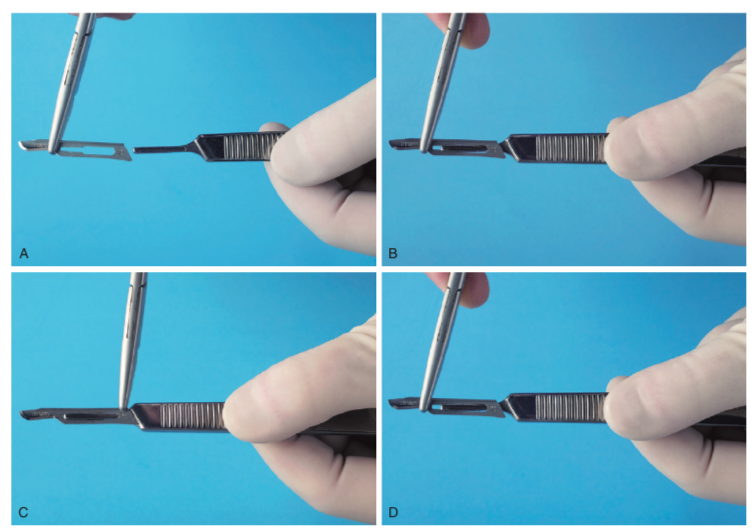
\includegraphics[width=6cm]{OMS_scalpel_handle.png}
%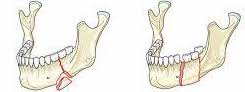
\includegraphics[width=5.5cm]{reduction_mandible.jpeg}
} % end of figure
{% text
\begin{outline}
\0 be careful focusing on
\1 attaching

\1 removing

    \2 scalpel handle and scalpel (SKAL-pel)
\end{outline}
} % end of text
%%
\clearpage

%\subsubsection{}


%%
% - is up text, + is down image
\wrapr{-1mm}{7}{9cm}{-8mm}
{% figure
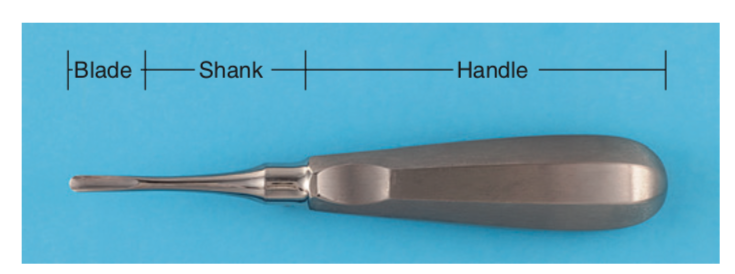
\includegraphics[width=6cm]{OMS_elevator.png}
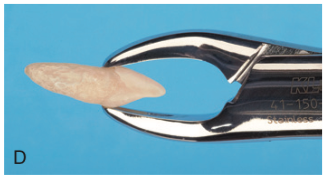
\includegraphics[width=3cm]{OMS_forceps_getTooth.png}
} % end of figure
{% text
\begin{outline}
\0 be careful holding
\1 a dental elevator

\1 placing on/between

    \2 bone and root of tooth
    \2 to ENGAGE it
\end{outline}
} % end of text
%%
\clearpage



% - is up text, + is down image
\wrapr{-8mm}{7}{6cm}{-5mm}
{% figure
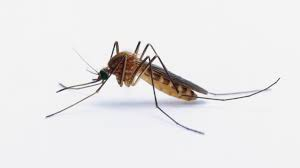
\includegraphics[width=2cm]{mosquito.png}
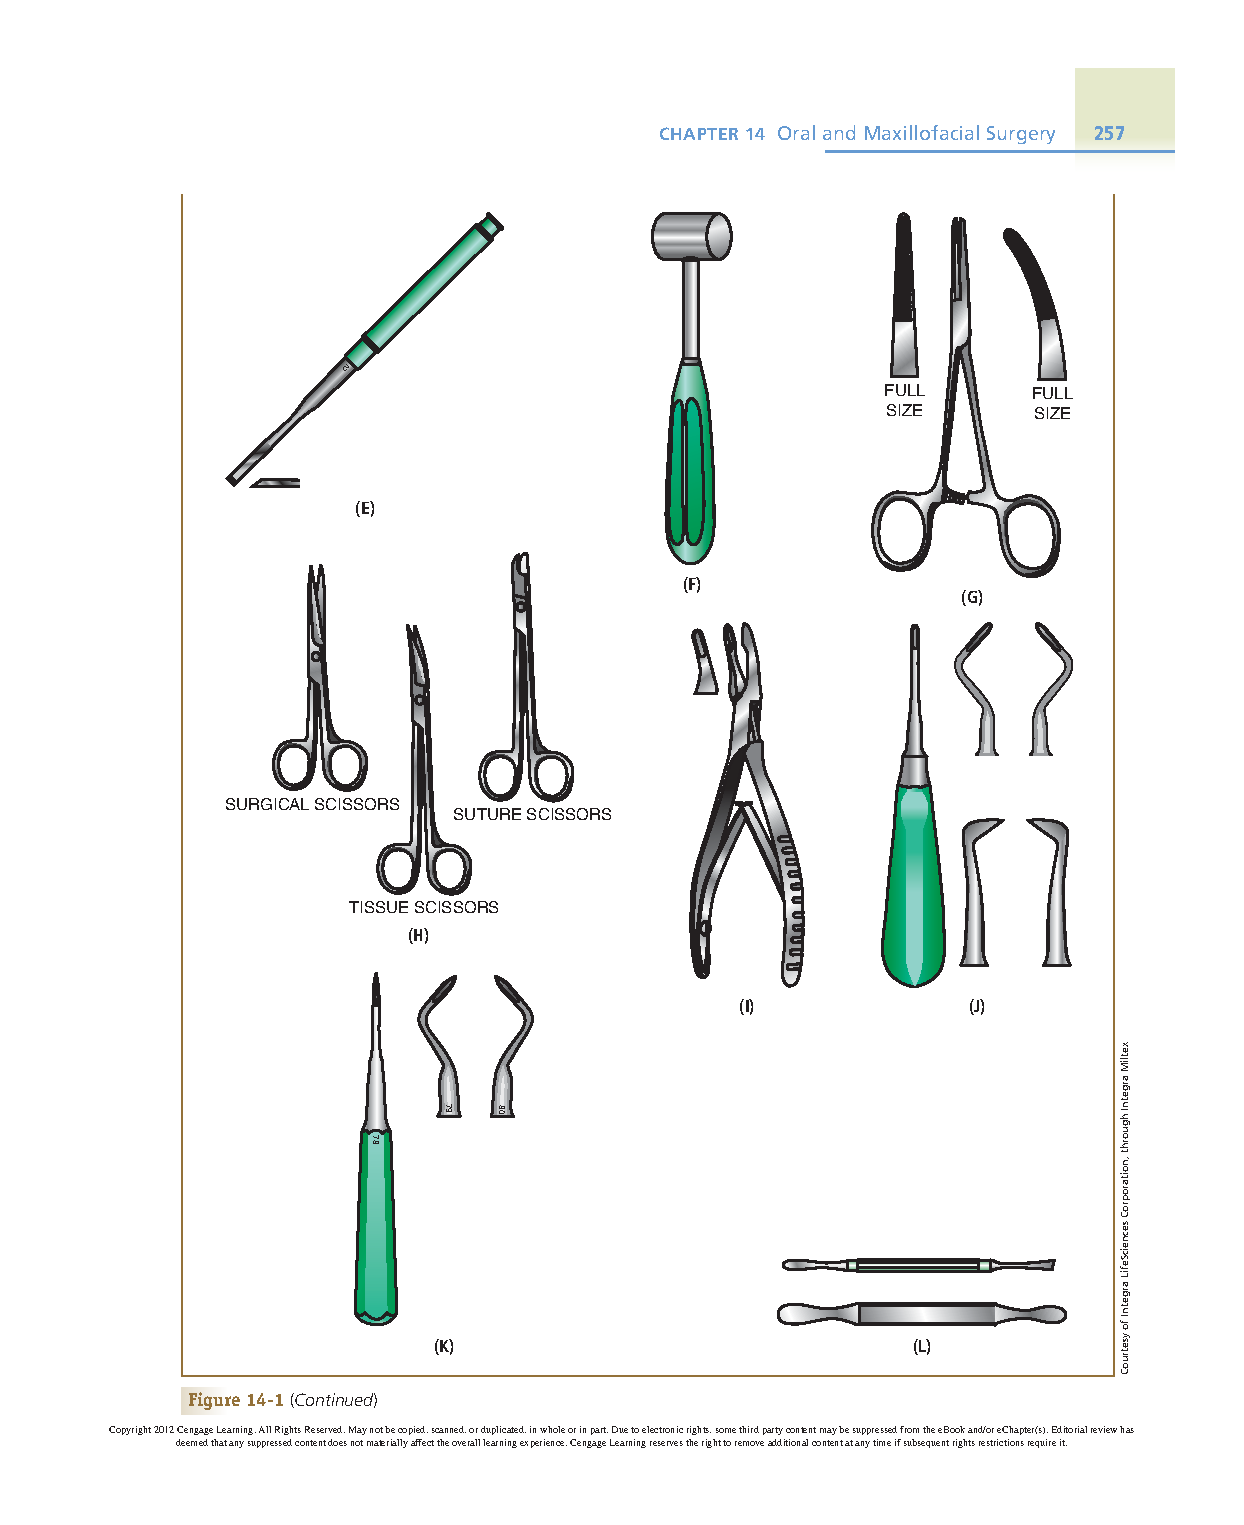
\includegraphics[width=5.5cm]{p257.pdf}

} % end of figure
{% text
\begin{outline}
\1 bone chisel and mallet (MAL-ett)
\1 hemostat (HE-moh-stat = mosquito)
\1 scissors x 3
\1 rongeurs (RON-jeers) forceps %\\[2mm]
\1 root elevator = exolever (ECKS-oh-lee-ver) elevator
\1 root tip elevator = apical elevator %\\[2mm]
\1 periosteal (pear-ee-OSS-tee-al) elevator(PE) = periosteotome  (pear-ee-OSS-tee-oh-tome)
\1 Seldin periosteal elevator
%Dingman elevator
\end{outline}
} % end of text


\clearpage
%%
\subsection{During radiotherapy}
 \subsubsection{Use of pilocarpine hydrochloride}
\begin{minipage}[c]{0.45\linewidth}
%\\
\begin{outline}
\0 for tooth/teeth removal
\1 single extraction (=1)
\2 simple
\2 impacted tooth
    \3 (A) horizontal impaction
    \3 (B) vertical impaction
    \3 (C) distoangular impaction
    \3 (D) mesioangular impaction
    \3 (E) transverse impaction
\end{outline}

\end{minipage}
\begin{minipage}[c]{0.5\linewidth}

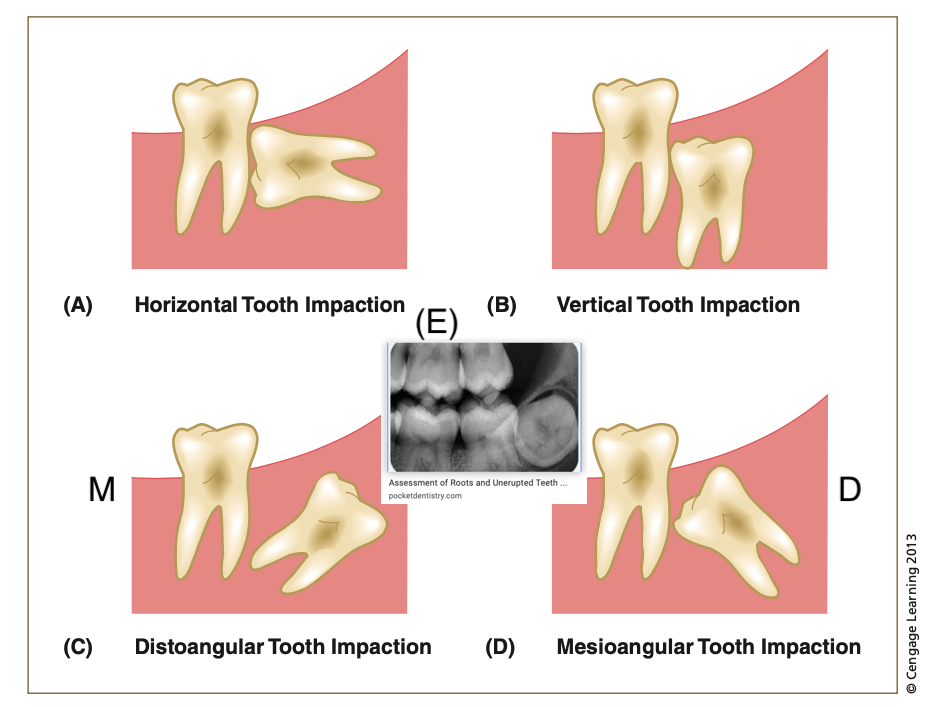
\includegraphics[width=8.0cm]{p258.png}
\end{minipage}

\clearpage
%%
\subsubsection{Oral care}

\begin{minipage}[c]{0.45\linewidth}
\begin{outline}
%\0 for teeth removal
\1 multiple extraction (>1)
\2 removal of alveolar bone crests: alveolectomy (al-vee-oh-LECK-toh-me)
\1 full mouth extraction (many teeth)
\2 guided with a surgical template  (TEM-plate = pattern)
\0 complication, such as
\1 inflammation of tooth socket: alveolitis (al-vee-oh-LIGH-tiss)
\1 "dry socket"

\end{outline}
\end{minipage}
\begin{minipage}[c]{0.5\linewidth}

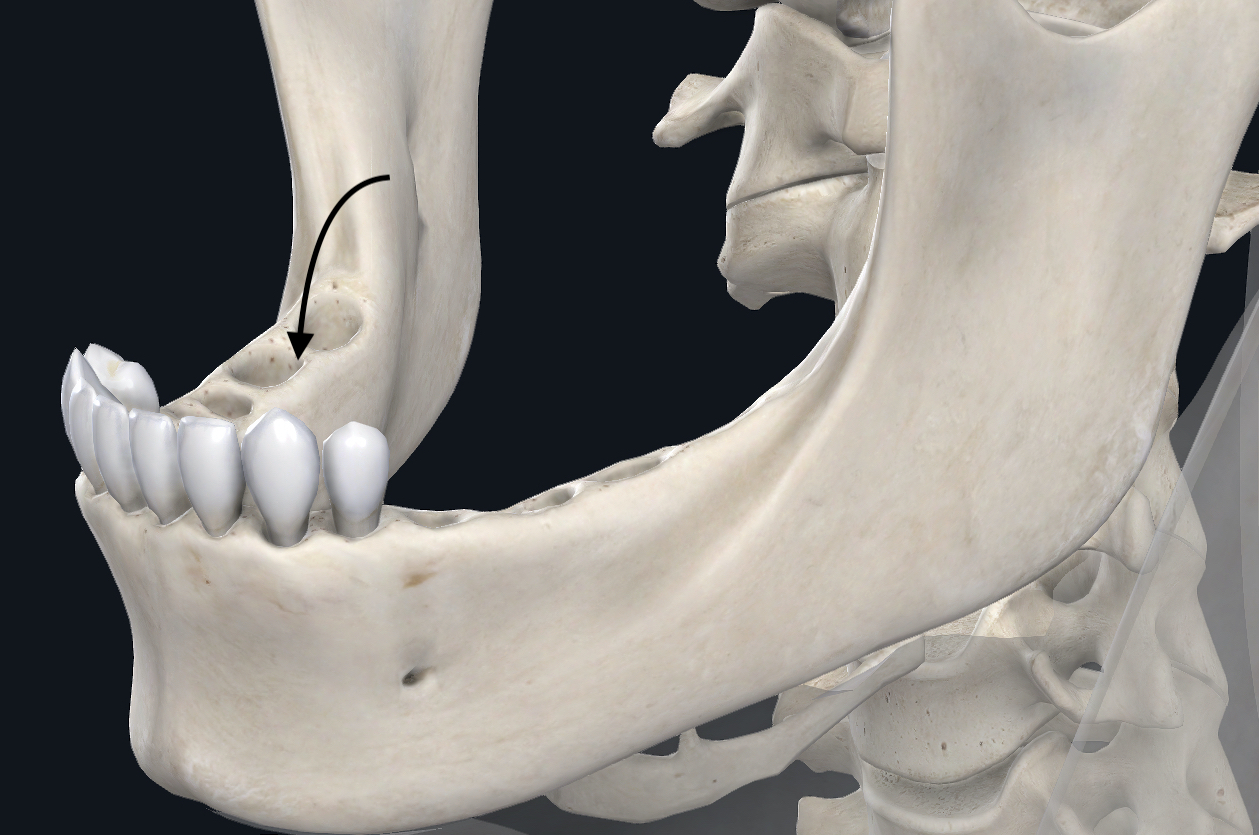
\includegraphics[width=4.5cm]{8272E96F-2F4C-4CA3-819B-C93D7E515B20.jpeg}
%\begin{figure}[!htb]
%    \centering
    \begin{tikzpicture}
    \node[anchor=south west,inner sep=0] (image) at (2,0) {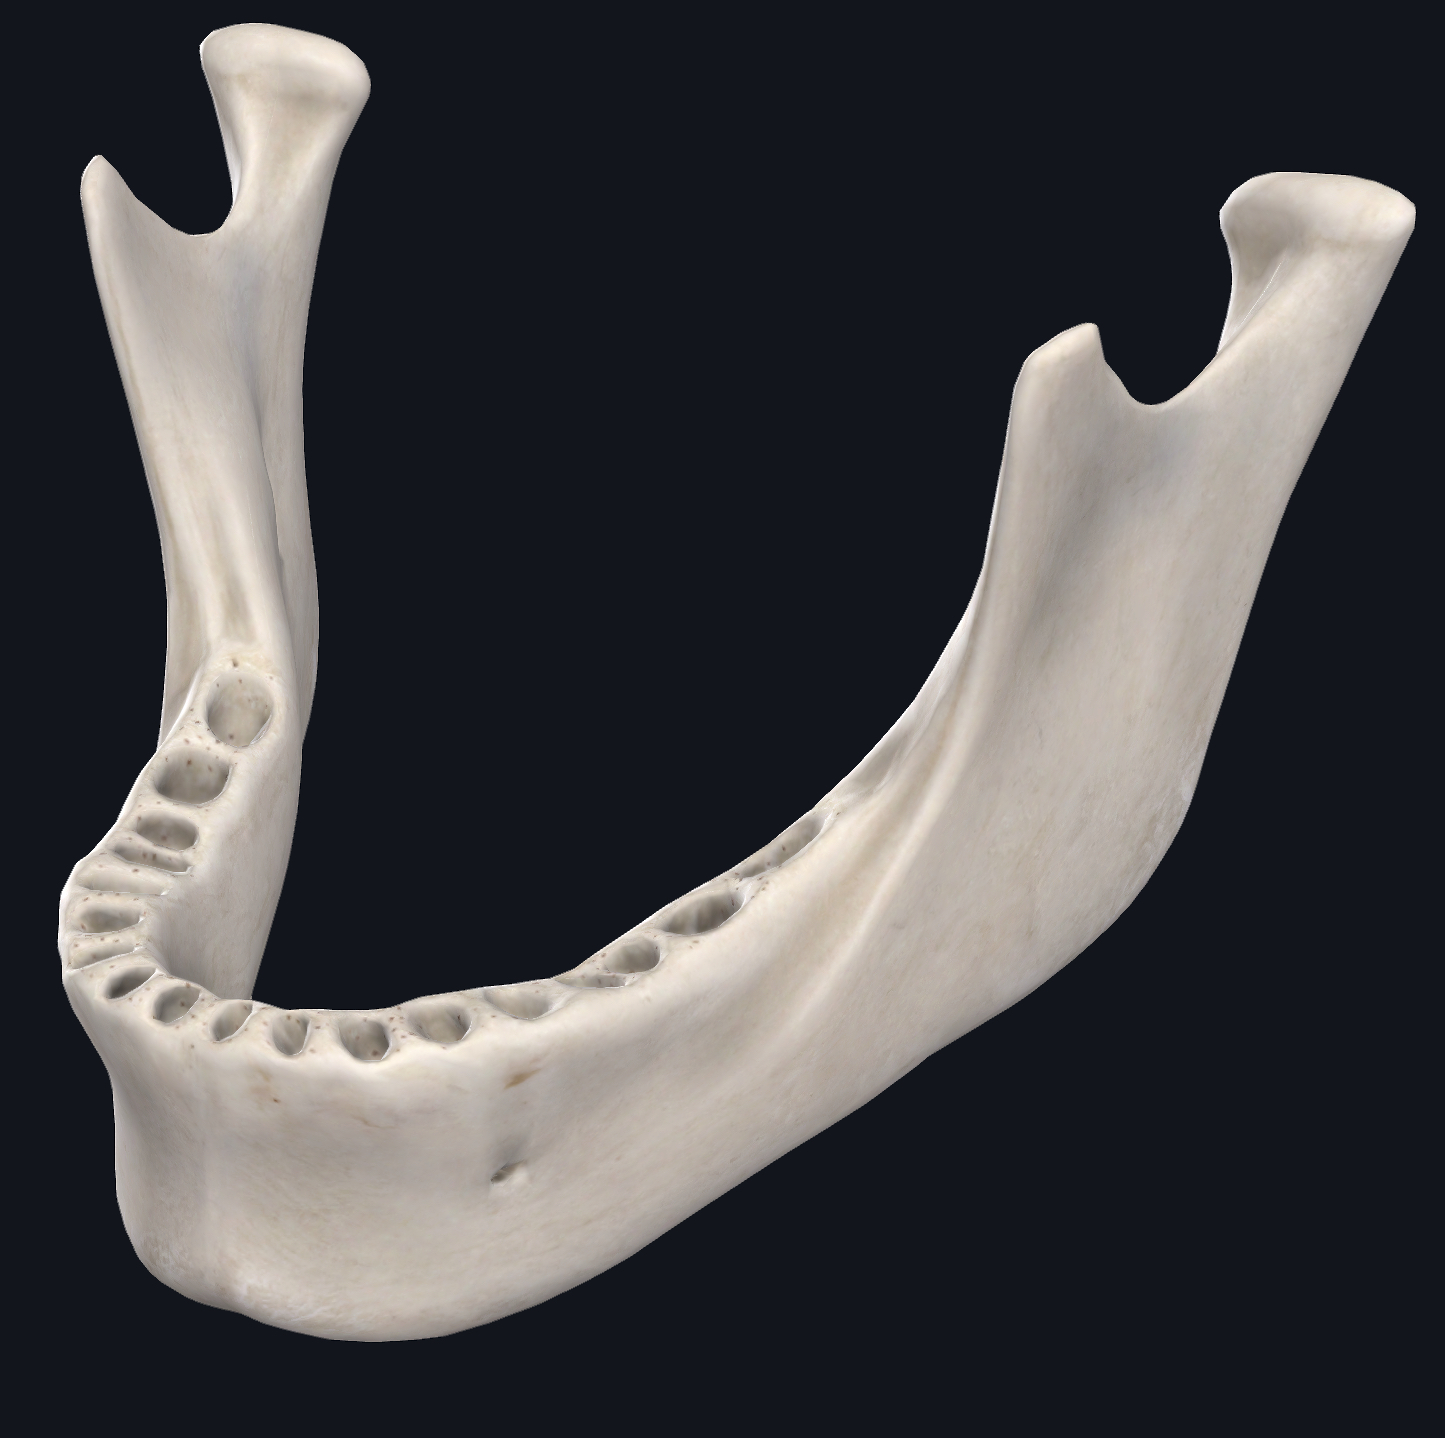
\includegraphics[width=4.0cm]{350D3956-2AD4-4C18-B38F-5DEC07BC59F8.jpeg}};

    \node[anchor=south west,inner sep=0] (image) at (2.5,2.7) {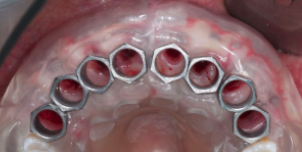
\includegraphics[width=0.3\textwidth]{template.png}};
    
    \node[anchor=south west,inner sep=0] (image) at (-0.5,-0.5) {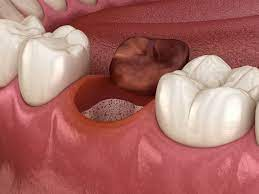
\includegraphics[width=0.3\textwidth]{dry_socket.png}};
    
    \end{tikzpicture}

%\end{figure}
\end{minipage}

\clearpage
%%
%\subsubsection{}


\subsection{Pathogenesis of oral mucositis}
Using dental elevator \\

Using dental forceps (= a pair of elevators) \\

%\clearpage
\subsubsection{Initiation of tissue injury}


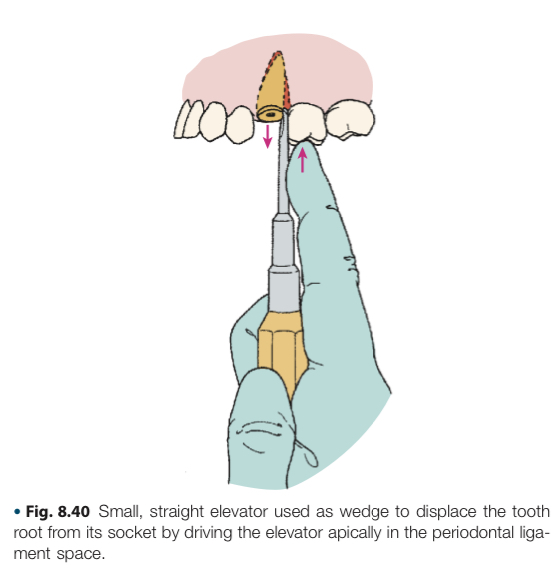
\includegraphics[width=0.5\textwidth]{709_elevators.jpg}

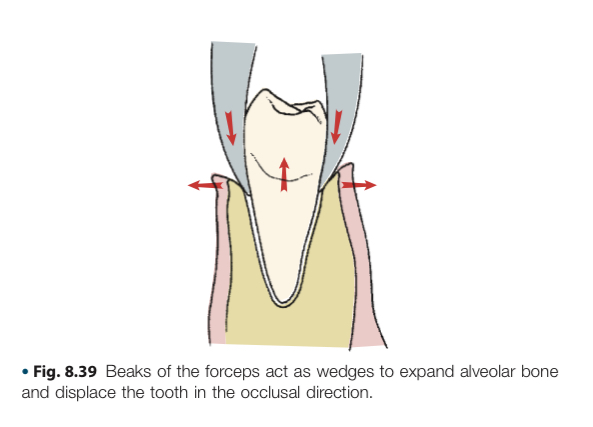
\includegraphics[width=0.70\textwidth]{31717_forceps.jpg}

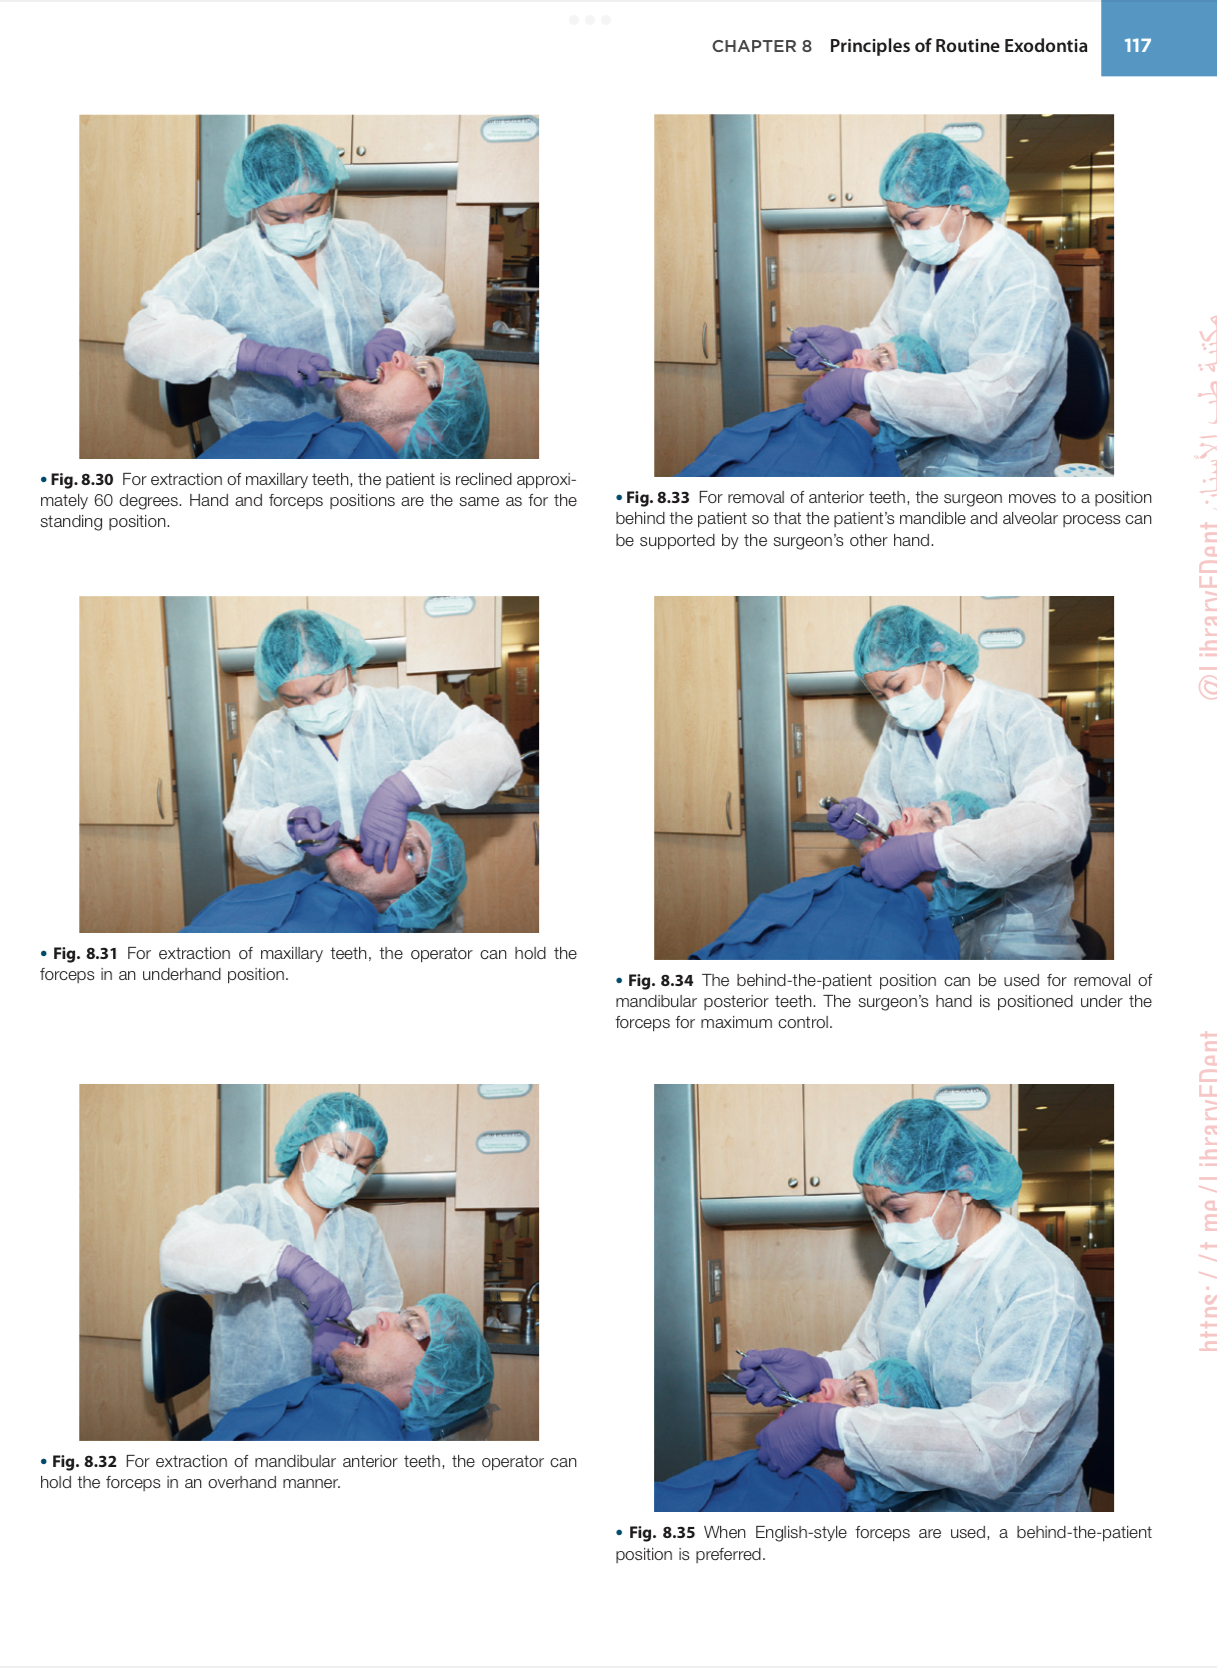
\includegraphics[width=0.40\textwidth]{89944_position_surgeon.jpg}

\clearpage
%%
\subsubsection{Upregulation of inflammation via generation of messenger signals}

\subsubsection{Ulceration and inflammation}

\subsubsection{Healing}
%%
\subsection{Clinical course of oral mucositis}

\begin{minipage}[c]{0.45\linewidth}

\begin{outline}
\1 gingivectomy (jin-jih-VECK-toh-me)
\1 gingivoplasty (jin-jih-voh-PLAS-tee)
\1 periodontal flap surgery for pericoronitis
\1 incision and drainage (I \& D) for odontogenic infection
\end{outline}
\end{minipage}
\begin{minipage}[c]{0.5\linewidth}



%\begin{outline}
    \begin{tikzpicture}
    \node[anchor=south west,inner sep=0] (image) at (3.7,0) {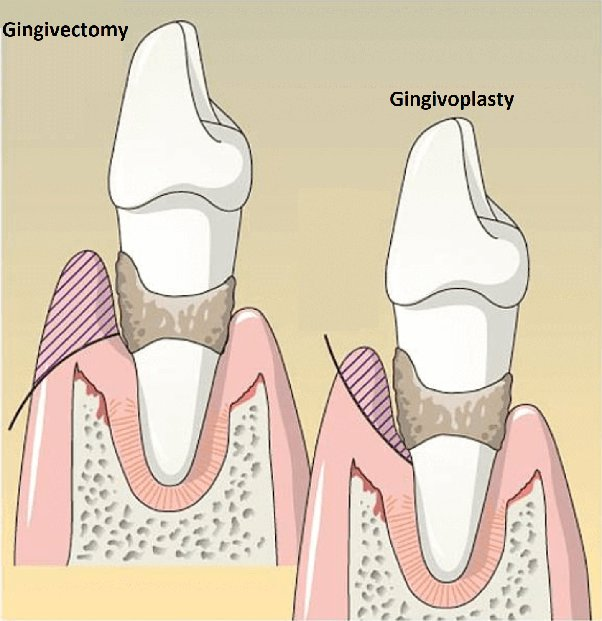
\includegraphics[width=4.0cm]{main-qimg-c0ad9eca21cd3a14caf6c883f4e44d6a-pjlq.jpeg}};

    \node[anchor=south west,inner sep=0] (image) at (-0.5,-0.7) {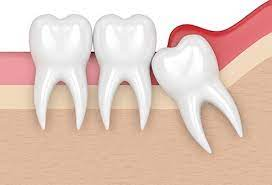
\includegraphics[width=0.5\textwidth]{pericoronitis.png}};
    
    \node[anchor=south west,inner sep=0] (image) at (-0.5,-2.7) {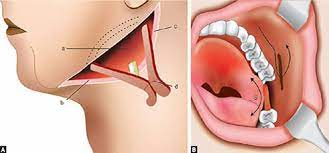
\includegraphics[width=0.5\textwidth]{incision_and_drainage.png}};
    
    \end{tikzpicture}

%\end{outline}
\end{minipage}


\clearpage
%%
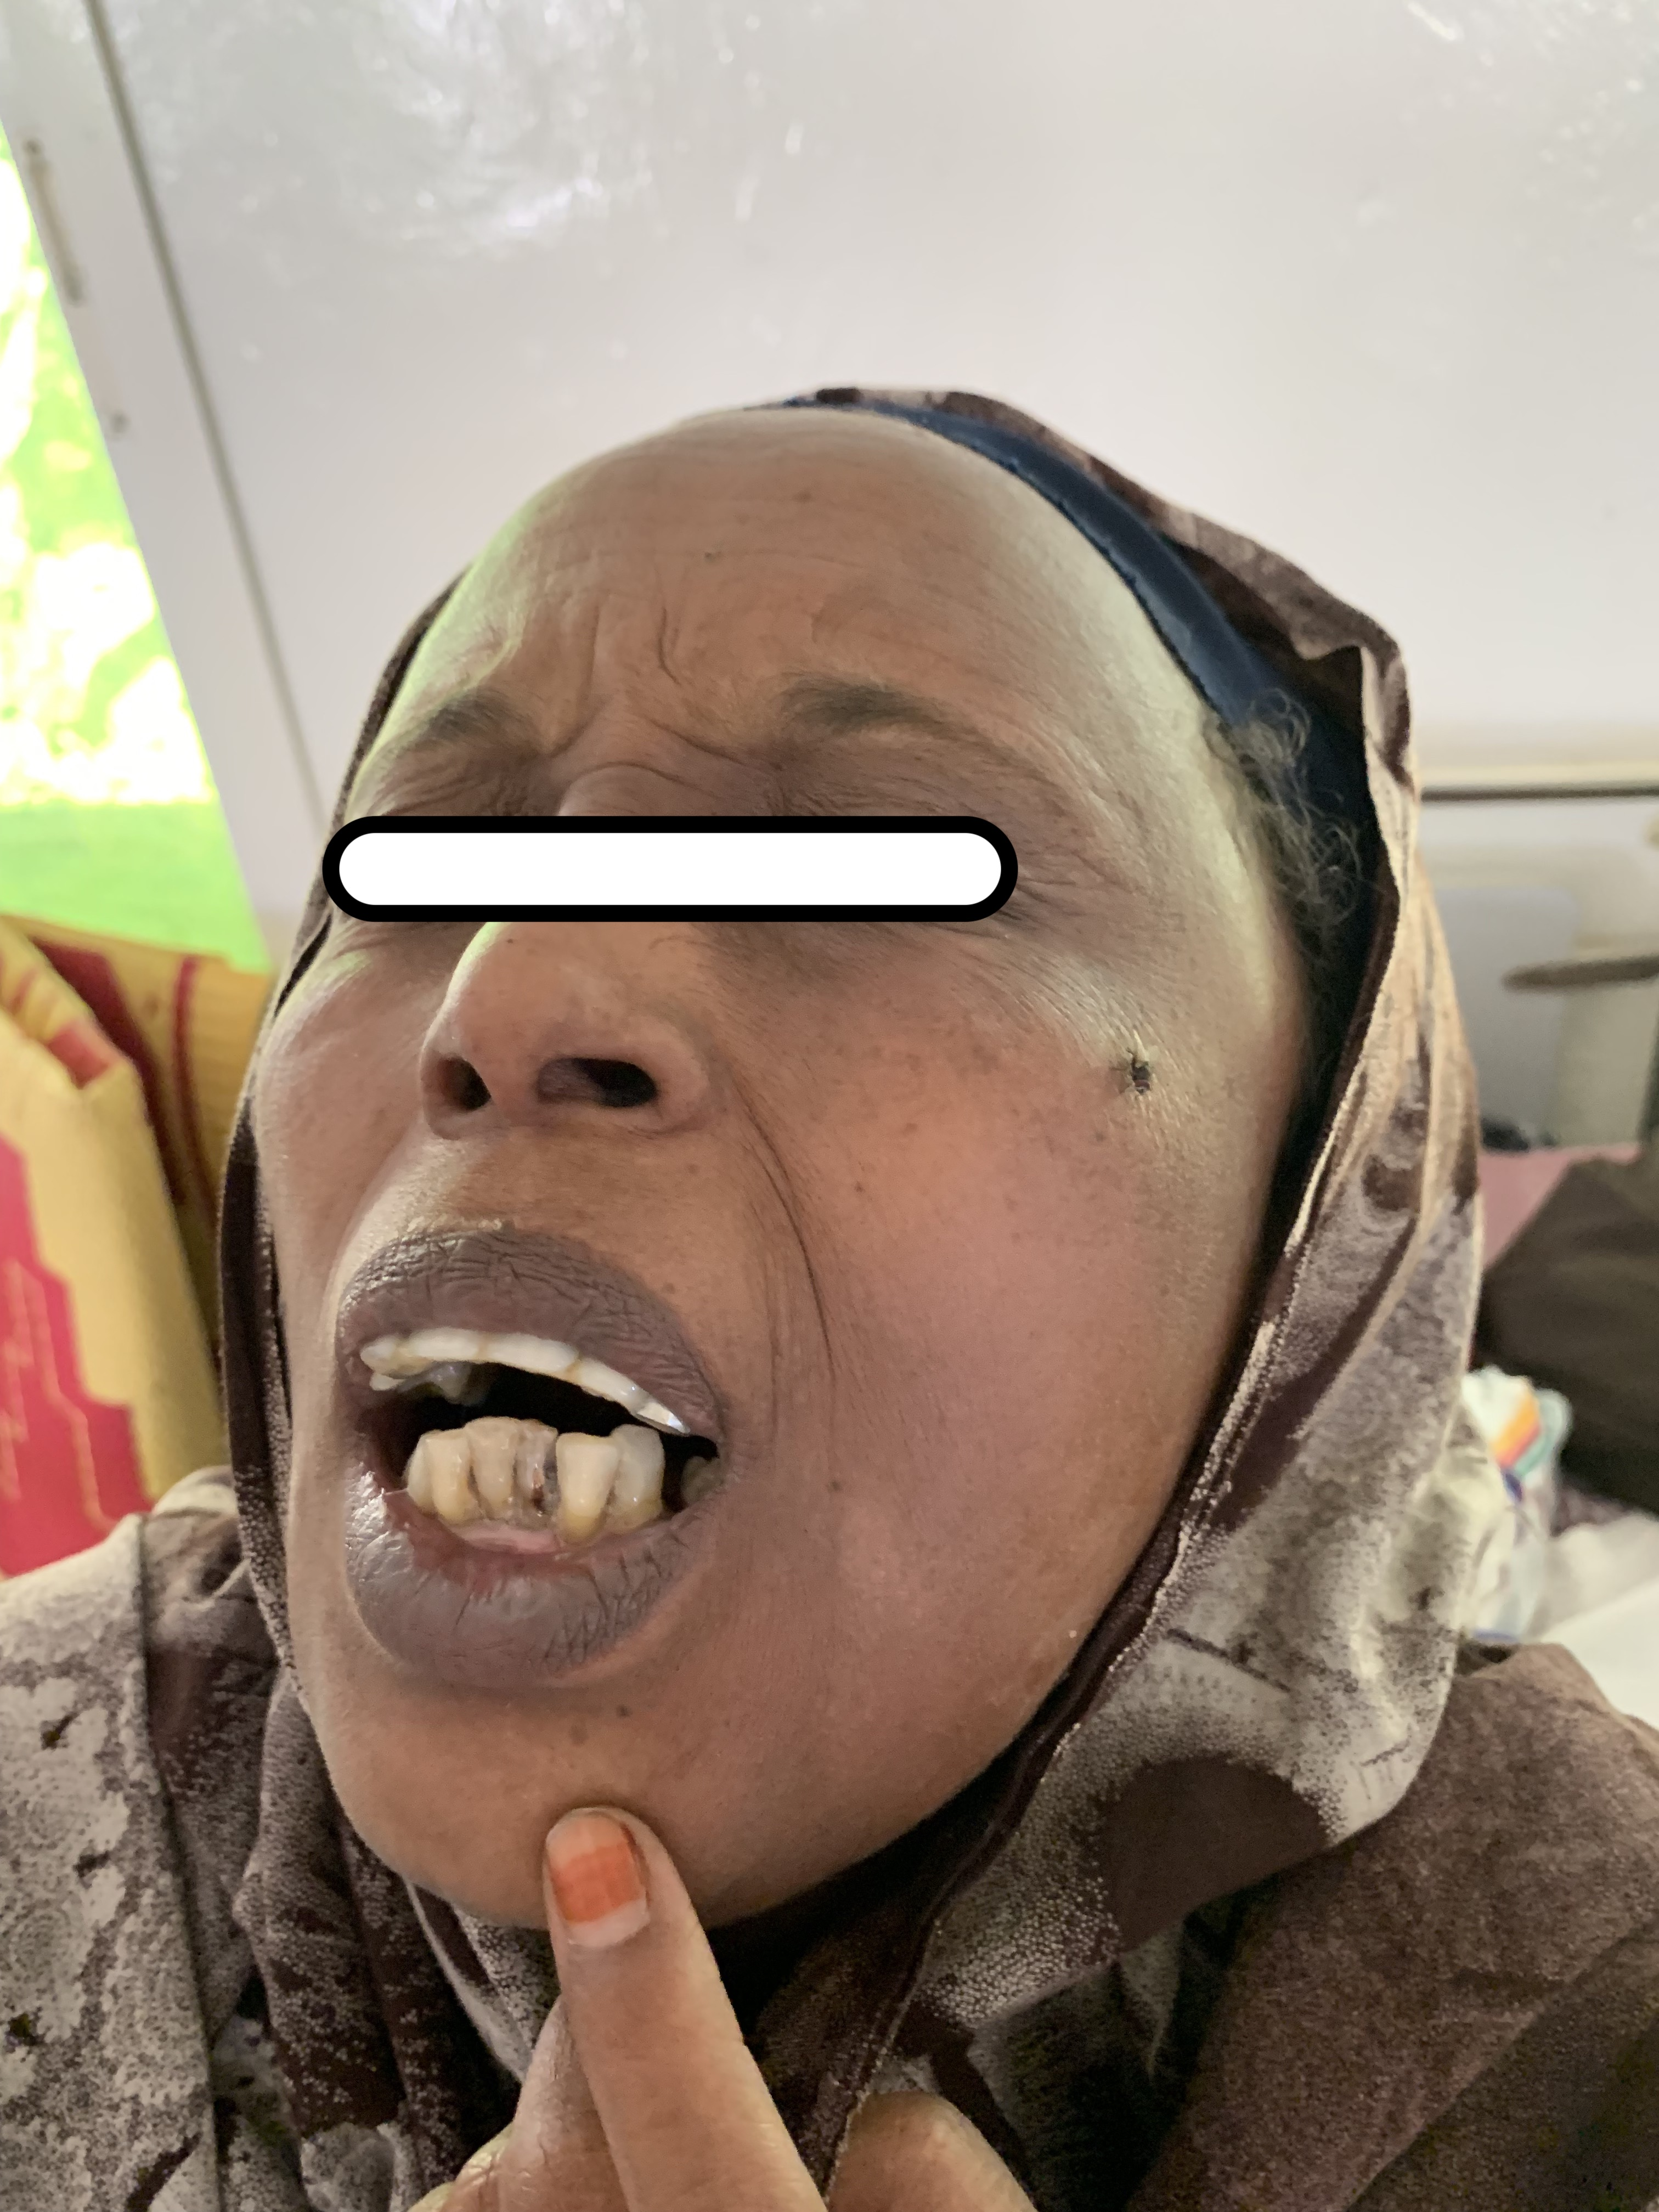
\includegraphics[width=5cm]{IMG_5180_photo_preOP_face.jpg}
\clearpage
%%
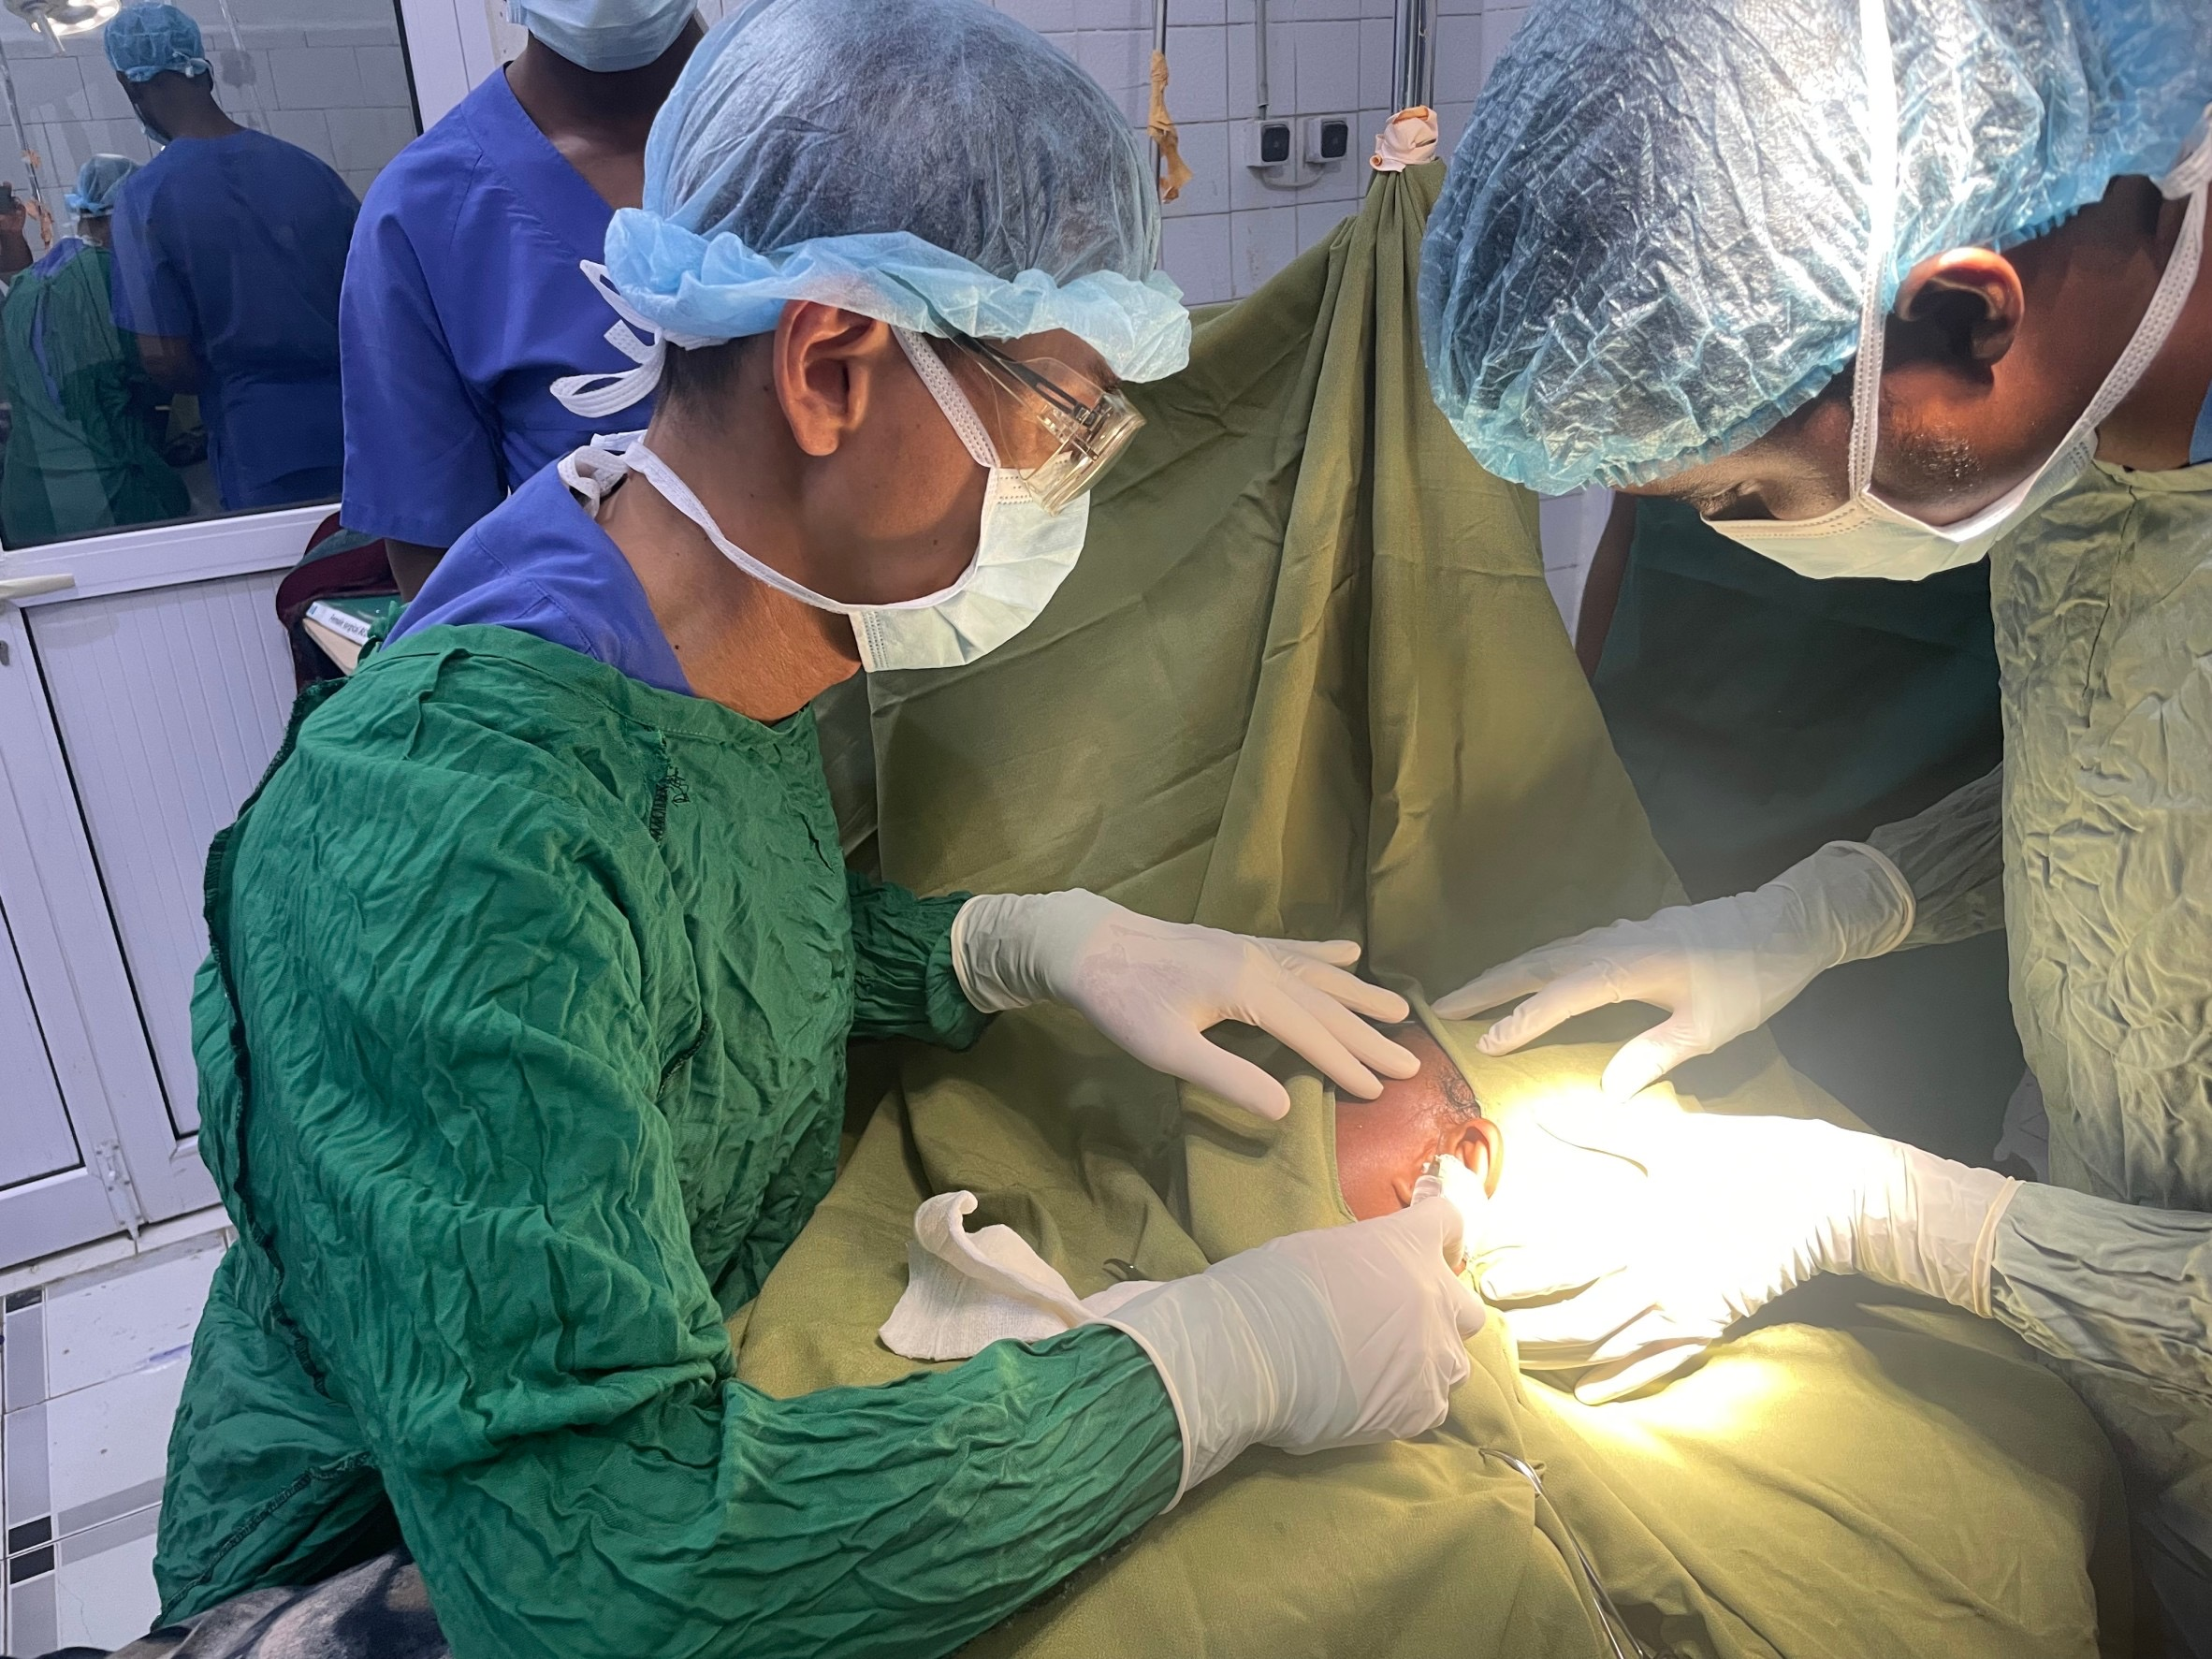
\includegraphics[width=8cm]{IMG_5286_localAnesthesia_IandD.JPG}


\clearpage
%%
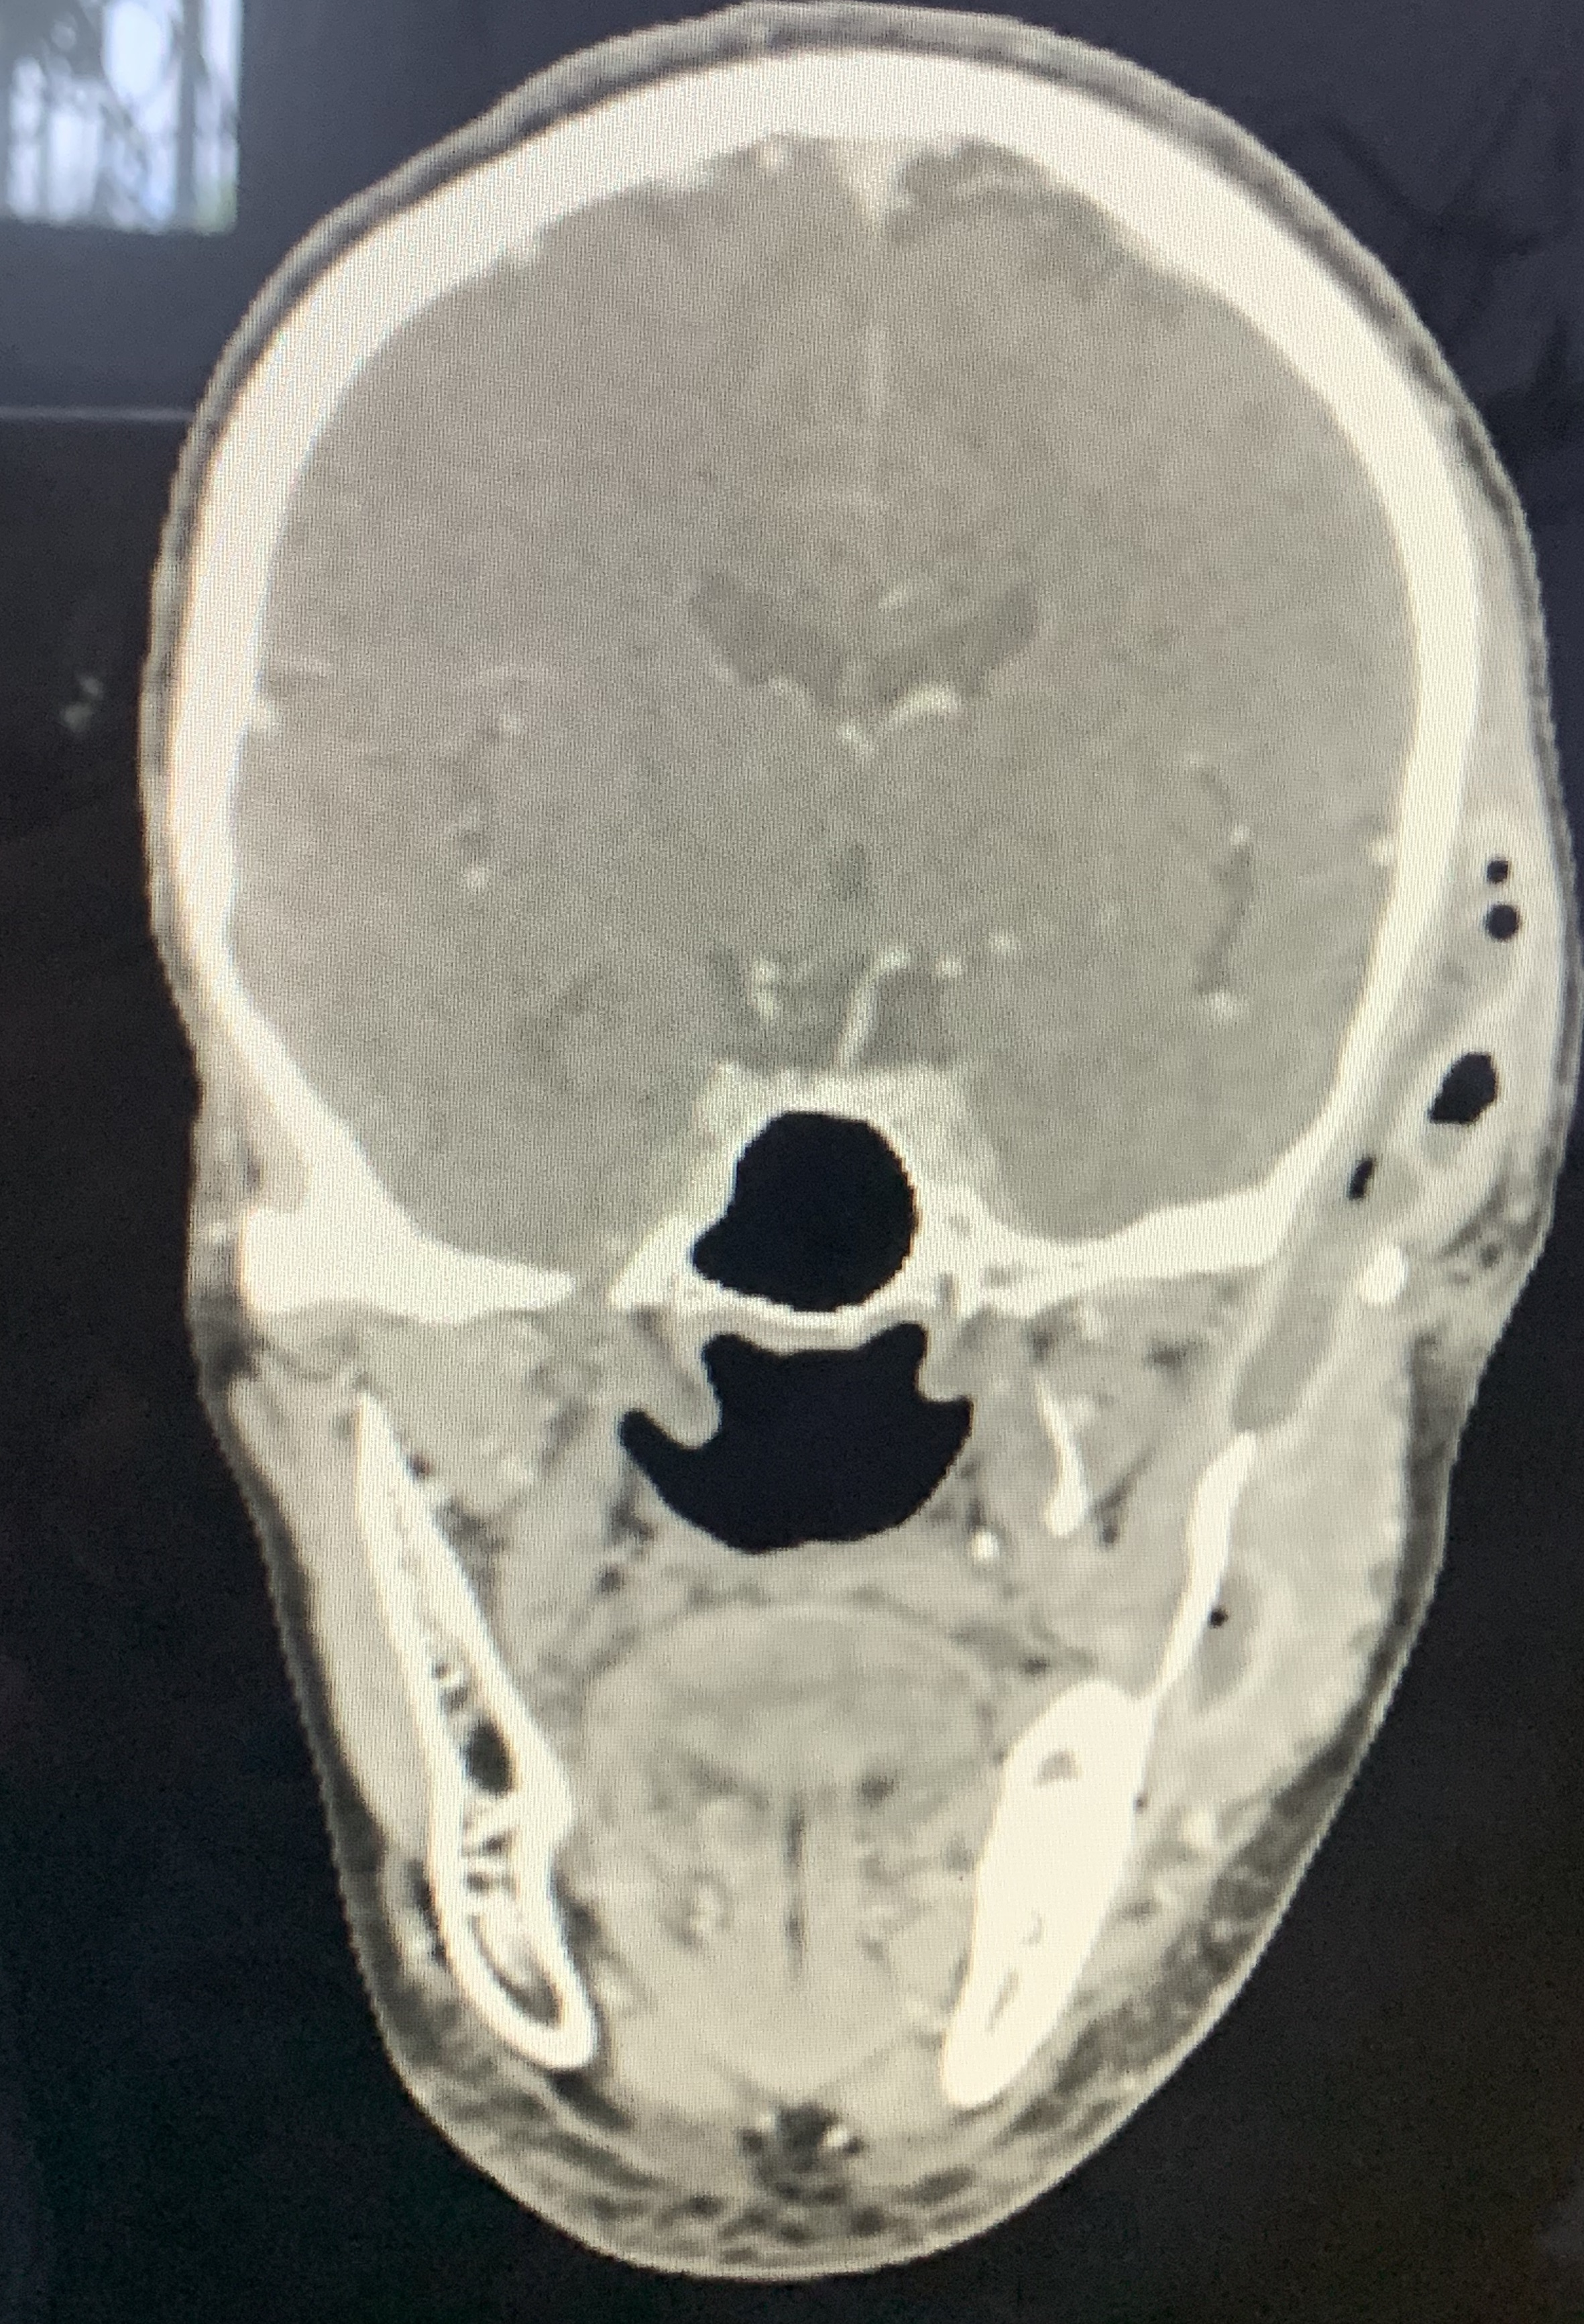
\includegraphics[width=5cm]{IMG_5296_CT_temporalAbscess.jpg}

\clearpage
%%
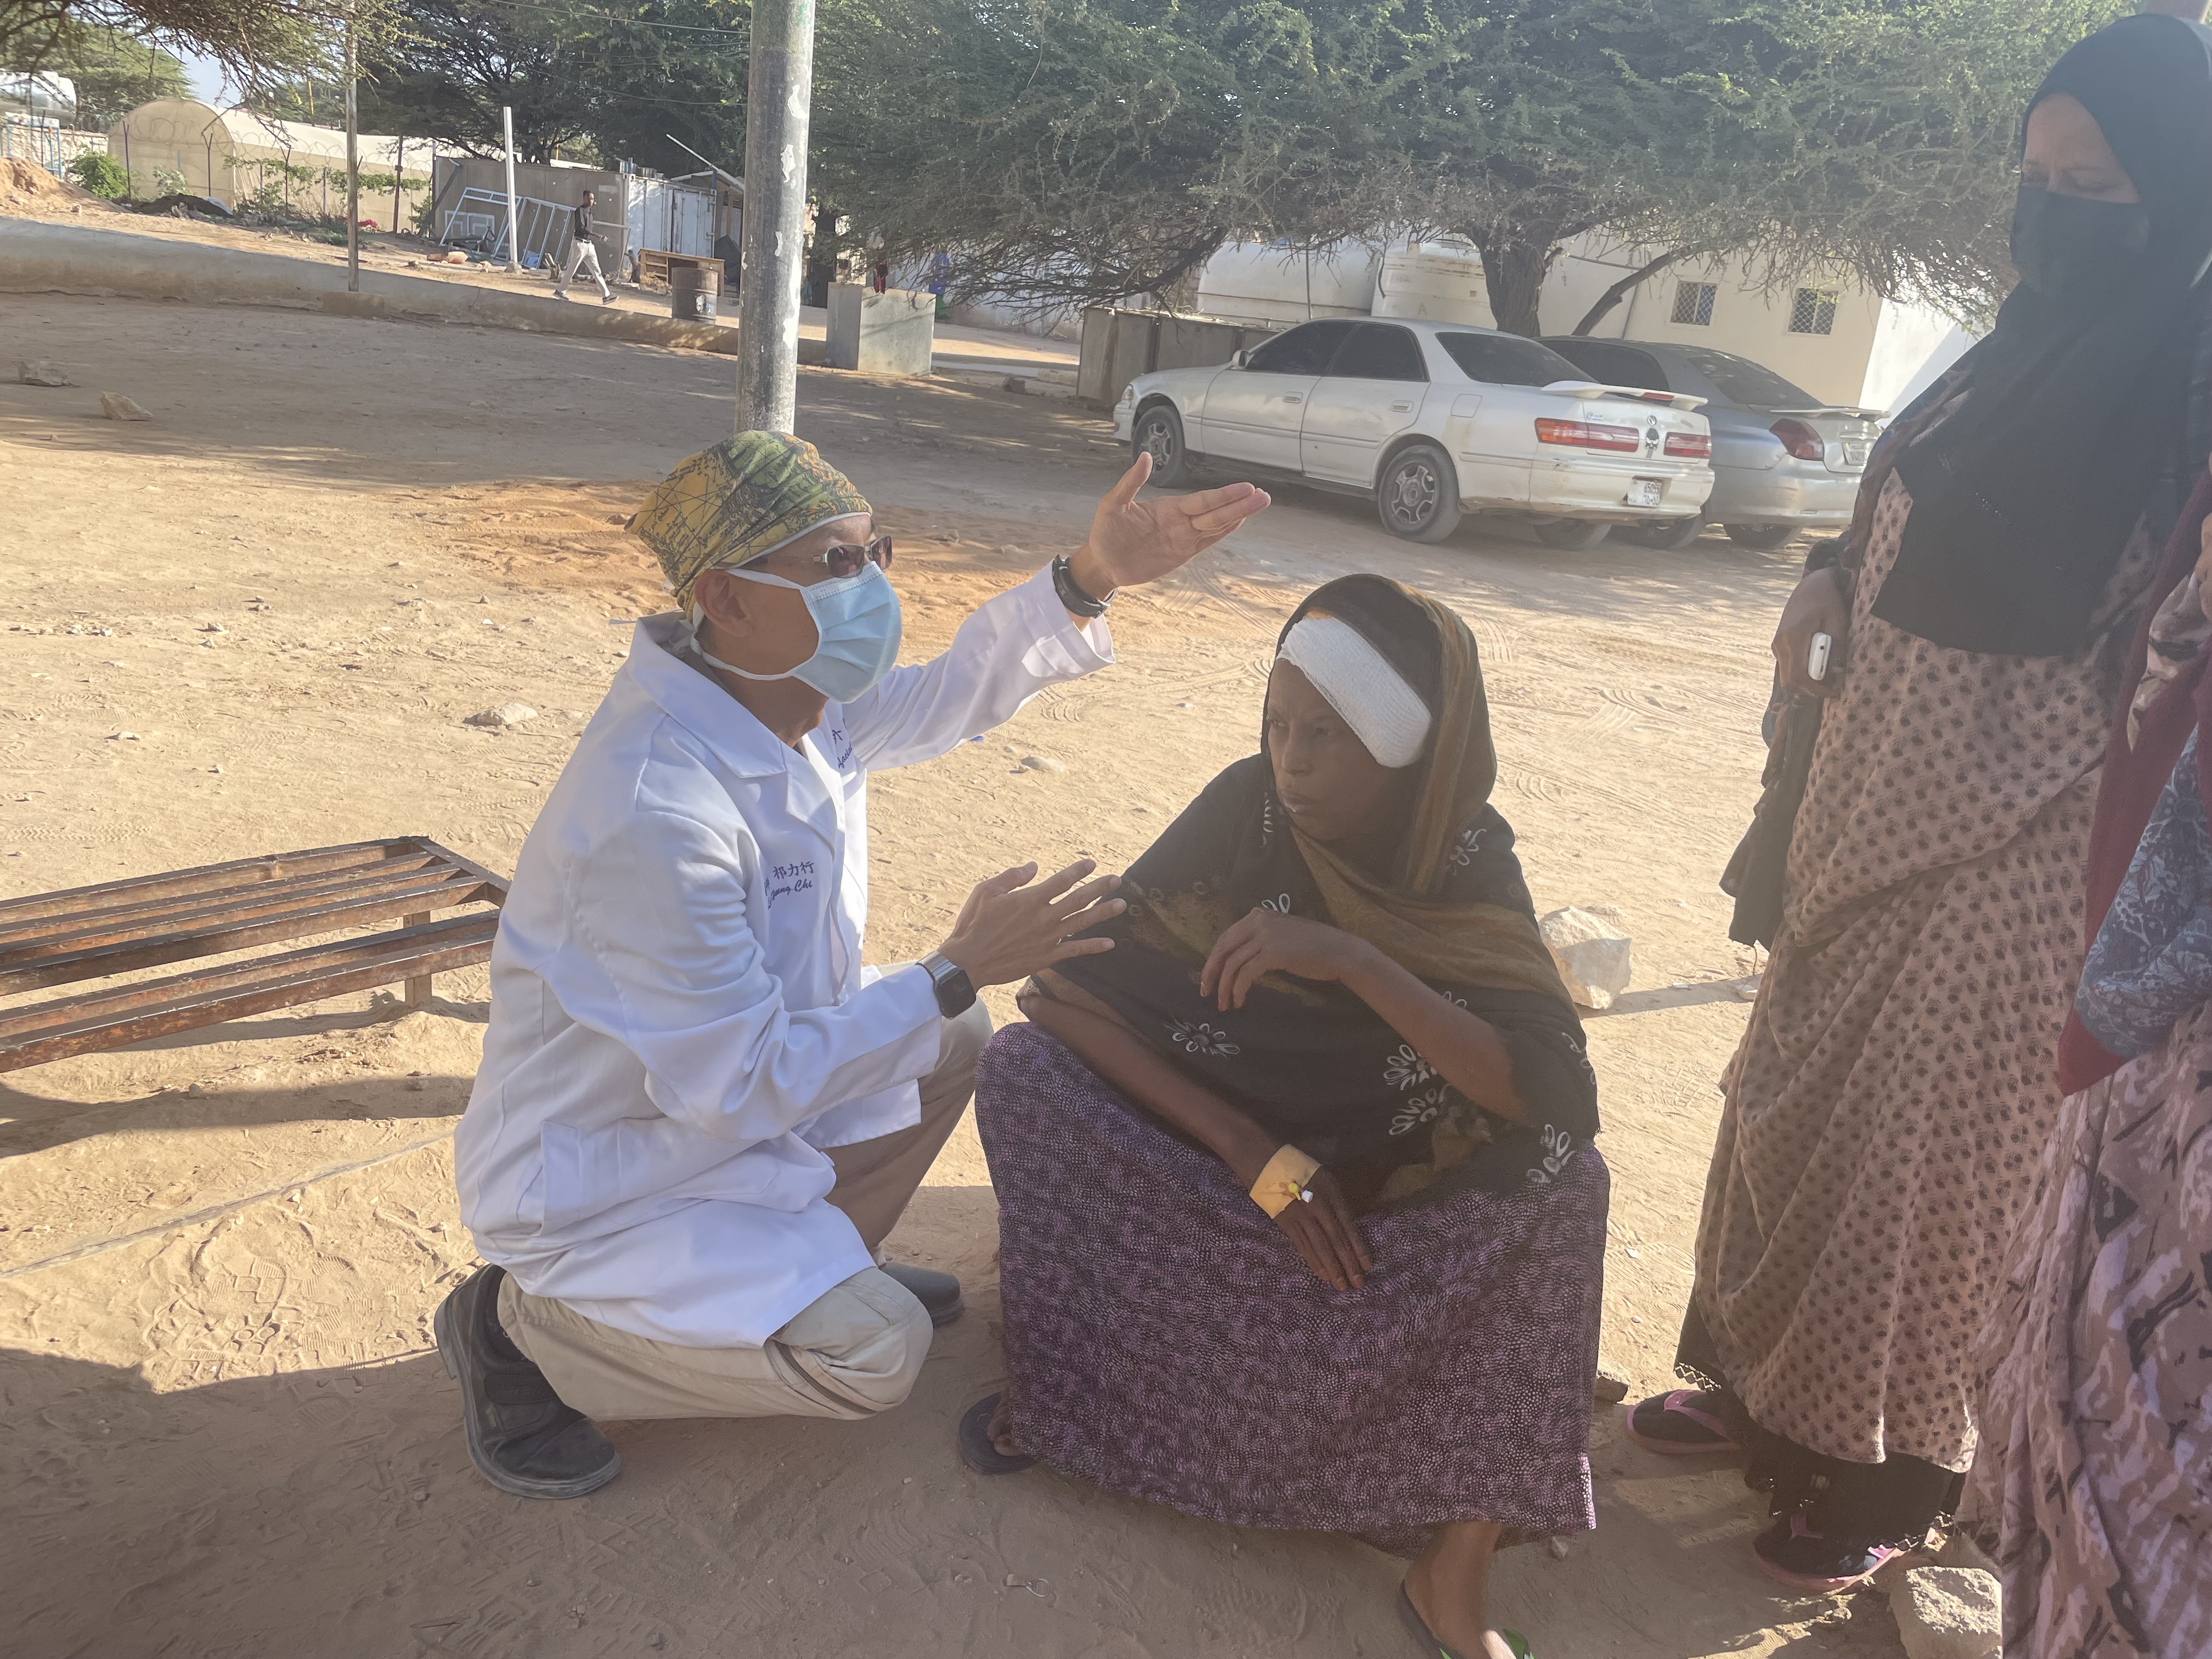
\includegraphics[width=9cm]{IMG_2114.JPG}
%%
\clearpage
%%
%%
\begin{minipage}[c]{0.6\linewidth}

\begin{outline}
\1 biopsy (BYE-op-see = small tissue incision)
    \2 incision biopsy (taken part of a lesion)
    \2 excision biopsy (taken all of it)
\1 lesions on oral mucosa
    \2 benign (bee-NINE = nonmalignant) tumors
        \3 granuloma (gran-you-LOH-mah)
        \3 fibroma
        \3 leukoplakia (loo-koh-PLAY-key-ah)
        \3 papilloma (pap-ih-LOH-mah)
        \3 hemangioma (he-man-jee-OH-mah)

    \2 malignant (mah-LIG-nant) tumors = cancer
        \3 squamous cell carcinoma
        \3 melanoma (mel-ah-NO-mah)
\end{outline}
\end{minipage}
\begin{minipage}[c]{0.4\linewidth}

    \begin{tikzpicture}
    \node[anchor=south west,inner sep=0] (image) at (0
    ,2.4) {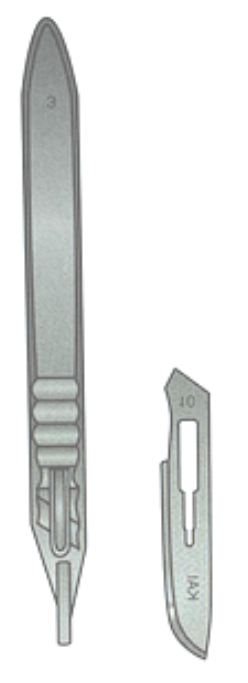
\includegraphics[width=1.2cm]{no10.png}};
    \node[anchor=south west,inner sep=0] (image) at (0,-1.4) {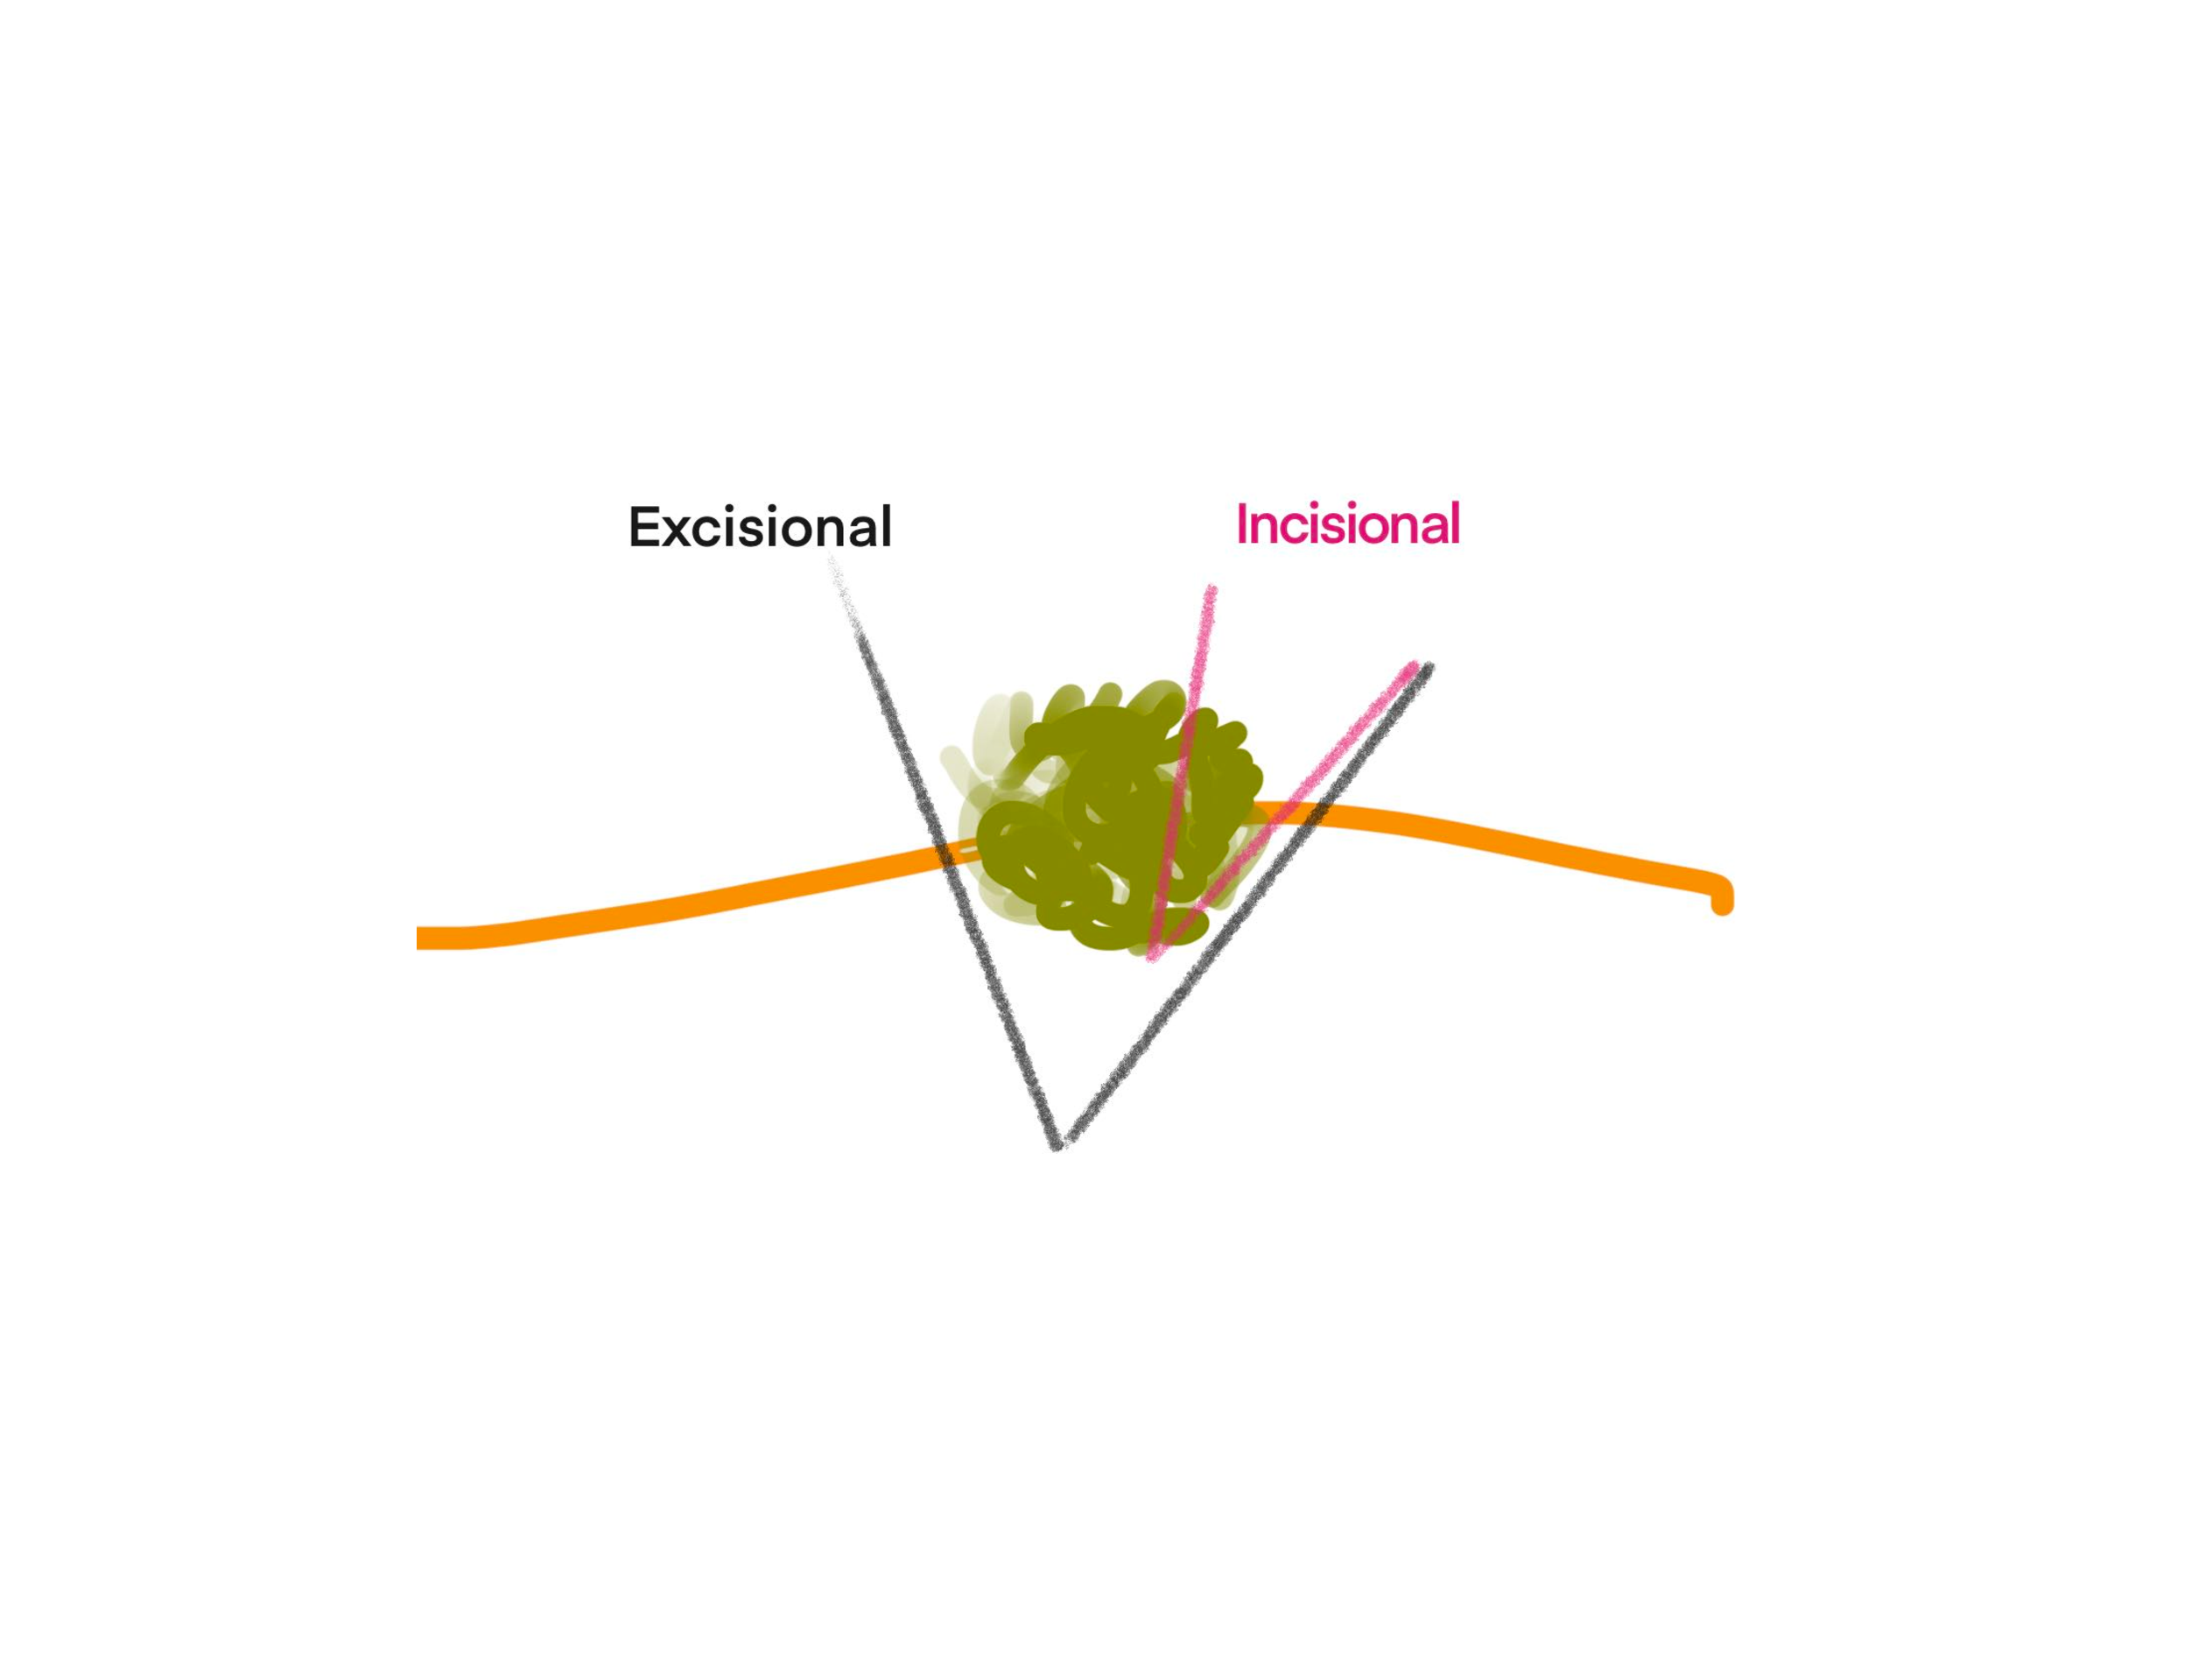
\includegraphics[width=7.0cm]{Biopsy.pdf}};

    \end{tikzpicture}
\end{minipage}


\clearpage
%%

\subsection{Evaluation of oral mucositis}

%      \begin{wrapfigure}[10]{r}{0.3\textwidth}
%      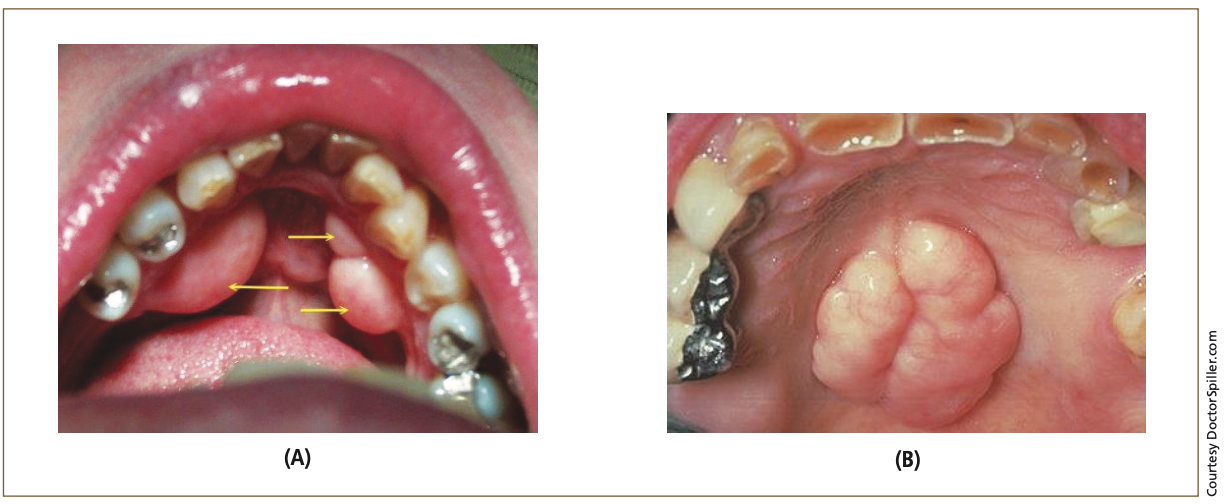
\includegraphics[width=6.5cm]{torus.png}
%      \end{wrapfigure}

% https://tex.stackexchange.com/questions/59101/will-it-ever-be-possible-to-use-wrapfig-with-an-enumerate-or-itemize-environment
% wrapl or wrapr{vertical adjustment of text}{number of lines}{horizontal space needed for the image}{vertical adjustment of image}{IMAGE}{TEXT}

% - is up text, + is down image
\wrapr{-10mm}{7}{6cm}{+16mm}
{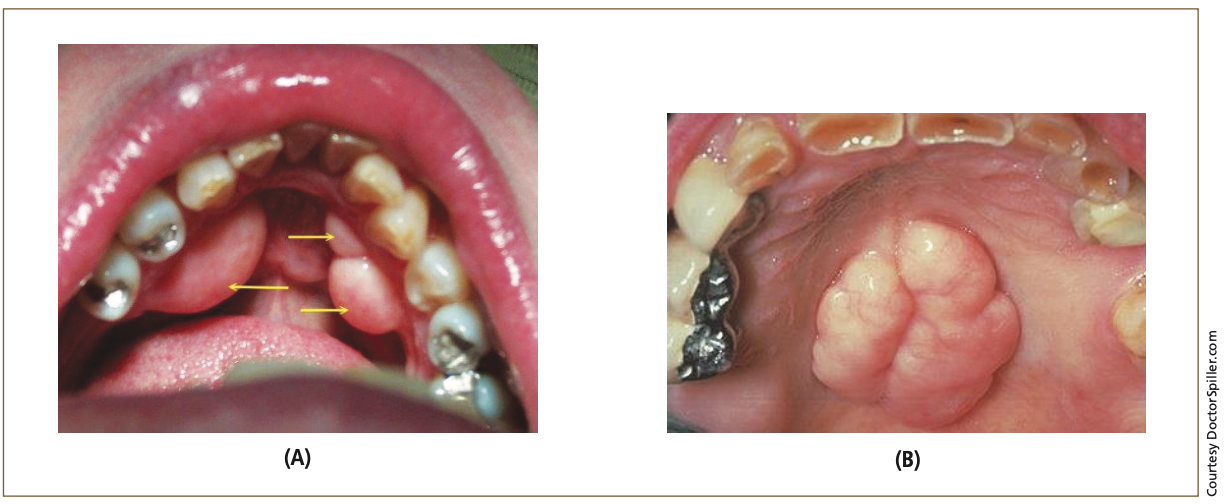
\includegraphics[width=6cm]{torus.png}}
{% text
\begin{outline}
\1 osteoplasty = OSS-tee-oh-plas-tee = forming or recontouring bones)
\1 alveolectomy (al-vee-oh-LECK-toe-mee)
\1 bone cutting for
%\end{outline}
%\begin{outline}
    \2 exostosis (ecks-ahs-TOH-sis = bony outgrowth)
    \2 torus (TORE-us = rounded elevation)
        \3 (A) torus mandibularis (man-dib-u- LAIR-iss)
        \3 (B) torus palatinus (pal-ah-TEEN-us
        
\end{outline}
} % end of text


%\end{minipage}
\clearpage
%%

% - is up text, + is down image
\wrapr{-8mm}{7}{6cm}{+8mm}
{% figure
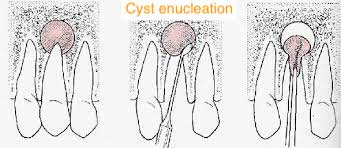
\includegraphics[width=5.5cm]{enucleation.jpeg}
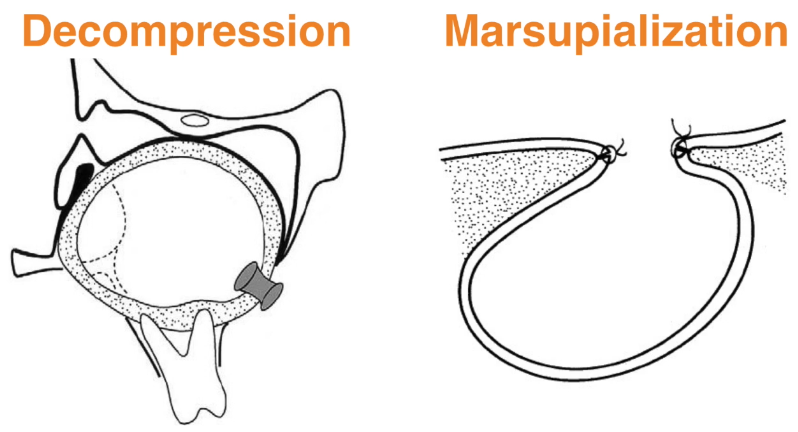
\includegraphics[width=5.5cm]{decompression.jpeg}
} % end of figure
{% text
\begin{outline}
\1 enucleation or decompression
    \2 cysts (SISTs = abnormal, closed-walled sac present in bone)
    \3 dentigerous (den-TIJ-er-us): cystic sac containing a crown of tooth
    \3 radicular (rah-DICK-you-lar): cyst located at the apex of a tooth root
\end{outline}
} % end of text

\clearpage
%
\subsection{Prevention and treatment of oral mucositis}

% - is up text, + is down image
\wrapr{-8mm}{7}{6cm}{-1mm}
{% figure
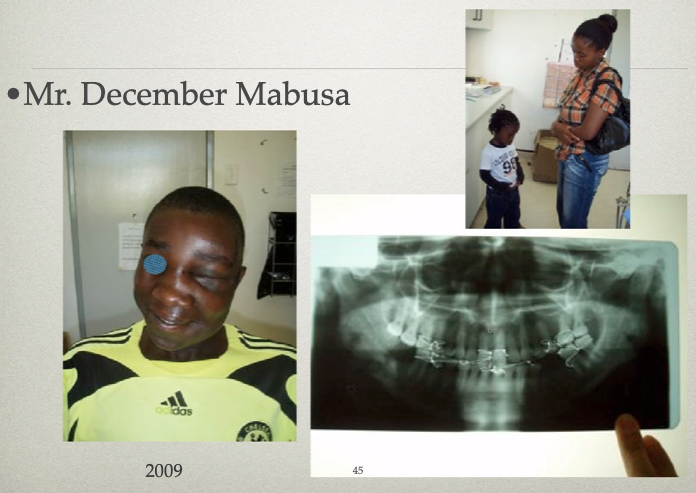
\includegraphics[width=5.5cm]{Mabusa.png}
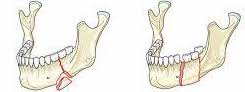
\includegraphics[width=5.5cm]{reduction_mandible.jpeg}
} % end of figure
{% text
\begin{outline}
\1 treatment
    \2 approaching, reduction, fixation, healing
\1  manner of reduction
    \2 closed fracture reduction
    \2 open fracture reduction
\end{outline}
} % end of text

\clearpage
%
\comm{  % we comment it out}
\subsection{Oral fungal infections}

An example: biopsy for Head and Neck Cancer

% phonetic spelling for native English speakers:
Oral verrucous hyperplasia (\acrshort{ovh}, vEr-uk-ohs hie-puh-plAY-ziuh) is a premalignant exophytic oral mucosal lesion with a predominantly verrucous or papillary surface; this lesion can subsequently transform into verrucous carcinoma (VC, vEr-uk-ohs kasi-NOUma), a well-established warty variant of squamous cell carcinoma (SCC, squa-mous sel kasi-NOUma).

%In \acrshort{ovh}, a predictive biomarker gives early alarm of its malignant transformation, which prevents unnecessary biopsy repeatedly.

%%%%%
\thispagestyle{headings}
%\markright{Introduction\hfill Oral cancer is a major disease in Taiwan \hfill}
%\begin{figure}
%\end{figure}



\begin{minipage}[c]{0.60\linewidth}
\begin{outline}
    \1 Head and neck squamous cell carcinoma (HNSCC) in Taiwan, which is:
        \2 derived from the \hl{oral cavity}, oropharynx, hypopharynx and larynx;
        \2 caused by long-term habits of betel nut \hl{[*OR 28.2]}, cigarette [*OR 18.0], alcohol [*OR 10.2]~\autocite{Ko1995}. {\tiny (*odds ratio)}
    \1  HNSCC is a serious problem in Taiwan:
%        \2 The \hl{sixth} common cancer worldwide~\autocite{Siegel2016};
        \2 The age-standardized incidence rate of \acrshort{hnscc} in males is \hl{42.15} per 100,000 person-years~ (7,400 victims/year) ~\autocite{MOHWincidence2018}**;
%        \2 Specialist of otolaryngology, oral and maxillofacial surgery in Taiwan (2021): 2,557 and 431, respectively  
        \2 The \hl{fourth} leading cause of cancer-related death for males in Taiwan (2,779 persons/year)~\autocite{MOHWdeath2017}**.
        {\tiny (*MOHW: Ministry of Health and Welfare, Taiwan)}
\end{outline}
\end{minipage}%\hspace{2mm}
%\begin{wrapfigure}{r}{0.3\textwidth}
\begin{minipage}[c]{0.35\linewidth}
    \raggedright
    \hfill
    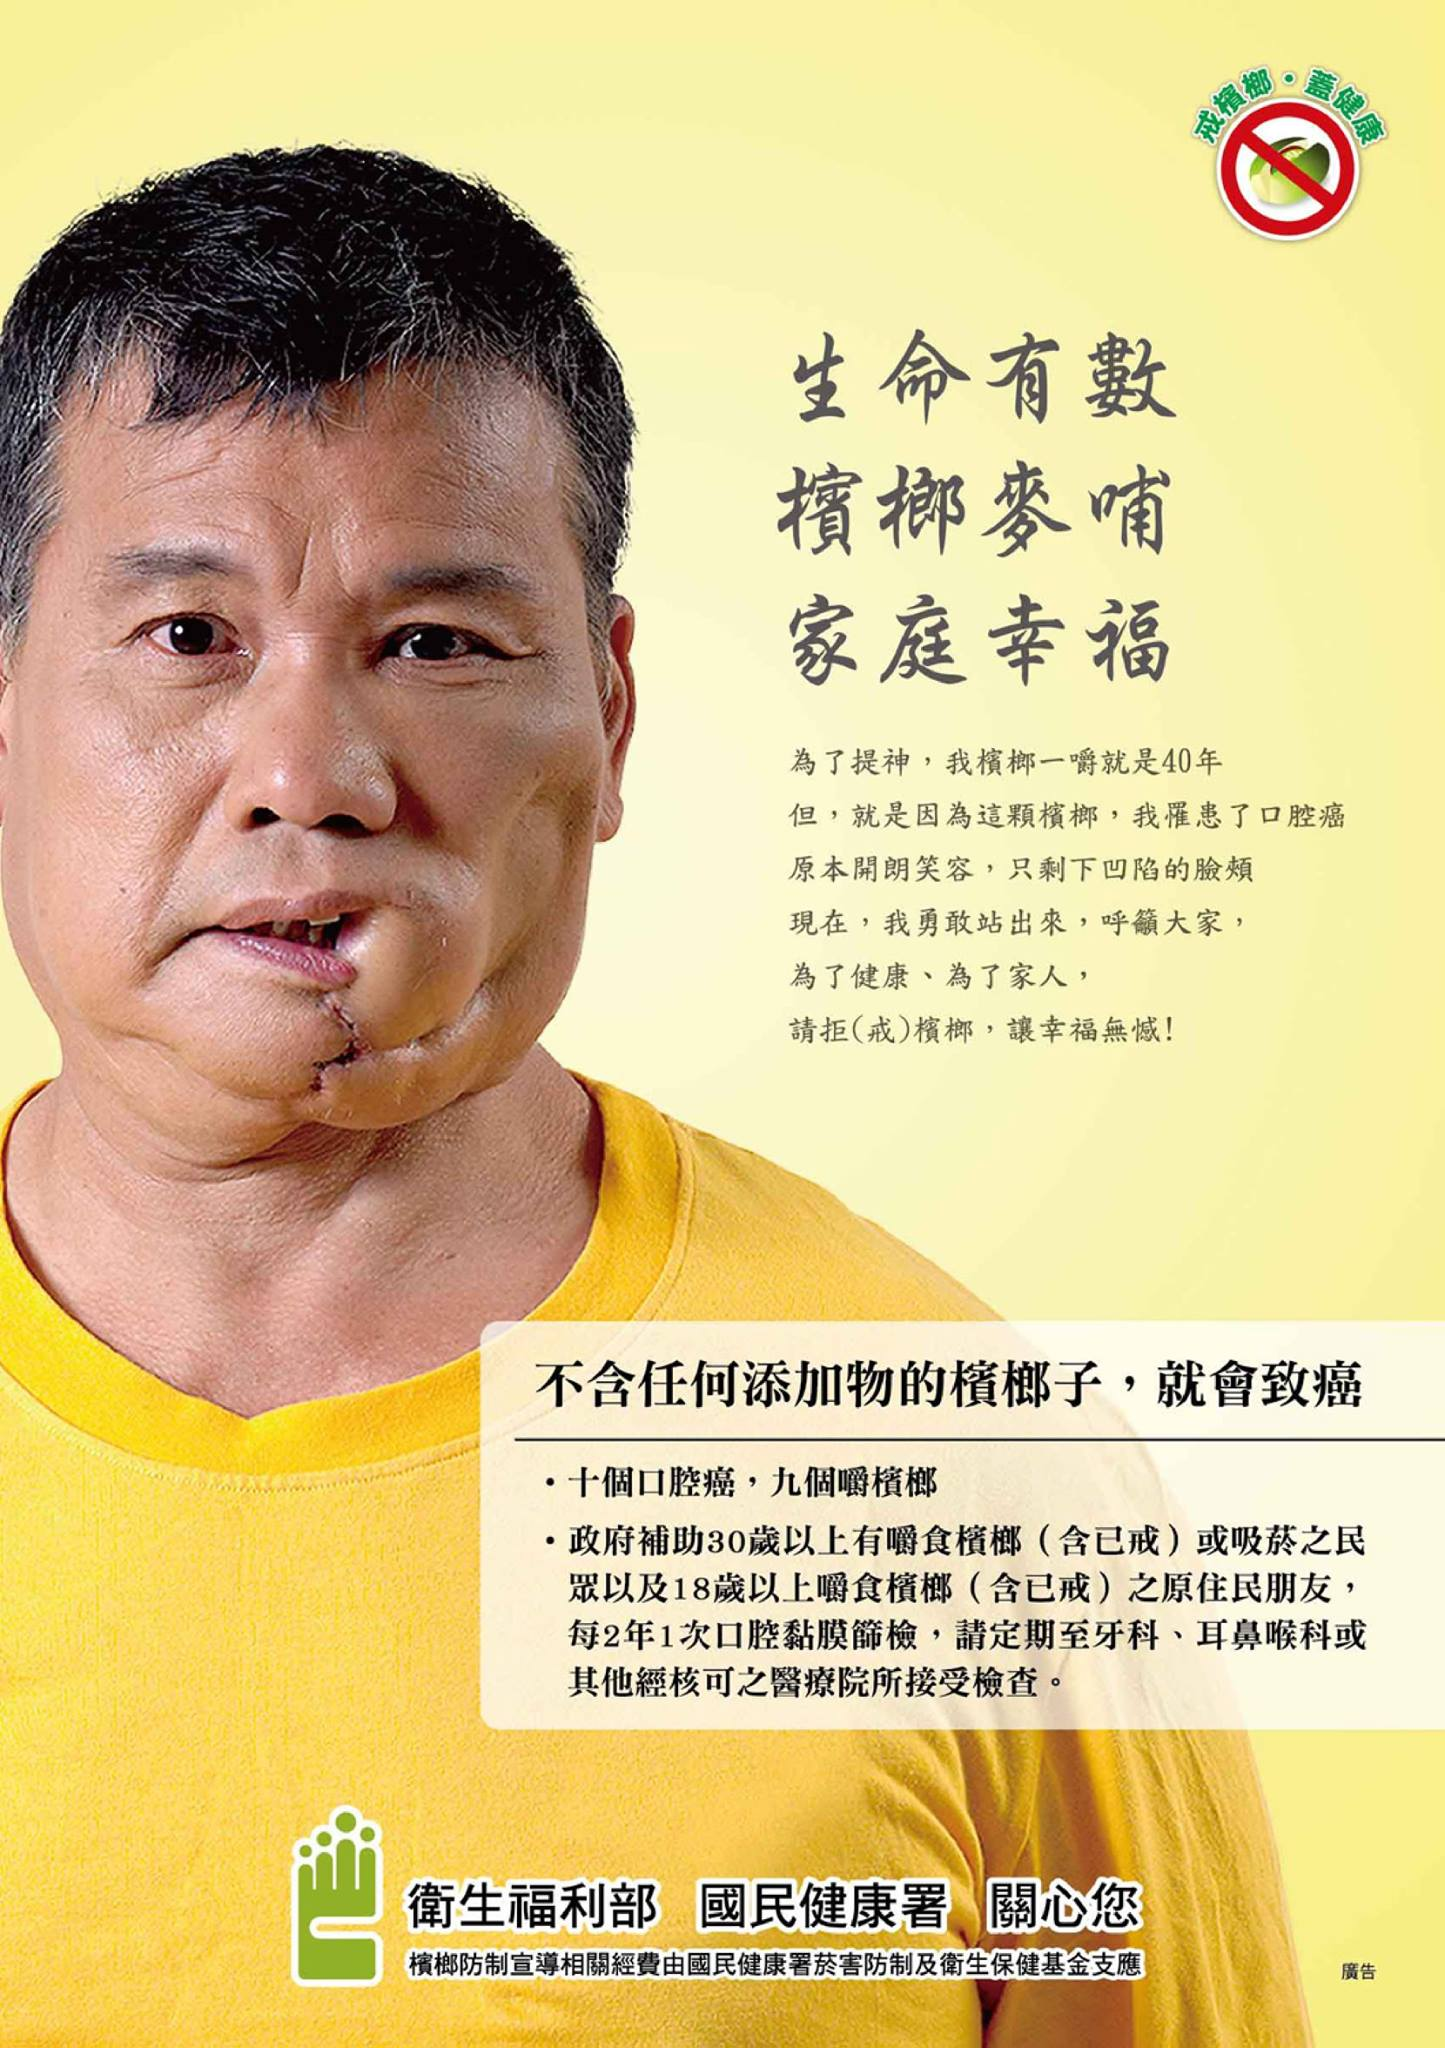
\includegraphics[width=4.5cm]{20369933_1755313531164078_5705495585669958017_o.jpg}\\
    %\caption*{
   \tiny (Photo courtesy of Health Promotion Administration, MOHW, Taiwan.)

\end{minipage}




\clearpage

%%%%%%%%%%%
\thispagestyle{headings}
%\markright{Introduction\hfill Biomarker-guided HNSCC therapy \hfill}

%The advantages of applying the TCGA data for cancer biomarker identification include:
\begin{outline}
\1  Treatment for HNSCC: \textcolor{green}{surgery}, radiotherapy, or systemic therapy (chemotherapy/targeted therapy)
%There are many physical and social features of patients available for survival modeling. % ($X_1 ... X_n$)
    \2 \hl{metastasis}: from oral cavity (T*) $\longrightarrow$ neck lymph nodes (N*) $\longrightarrow$ the rest of body (M*) (e.g., lung, liver, bone)
    

\begin{figure}
    \centering
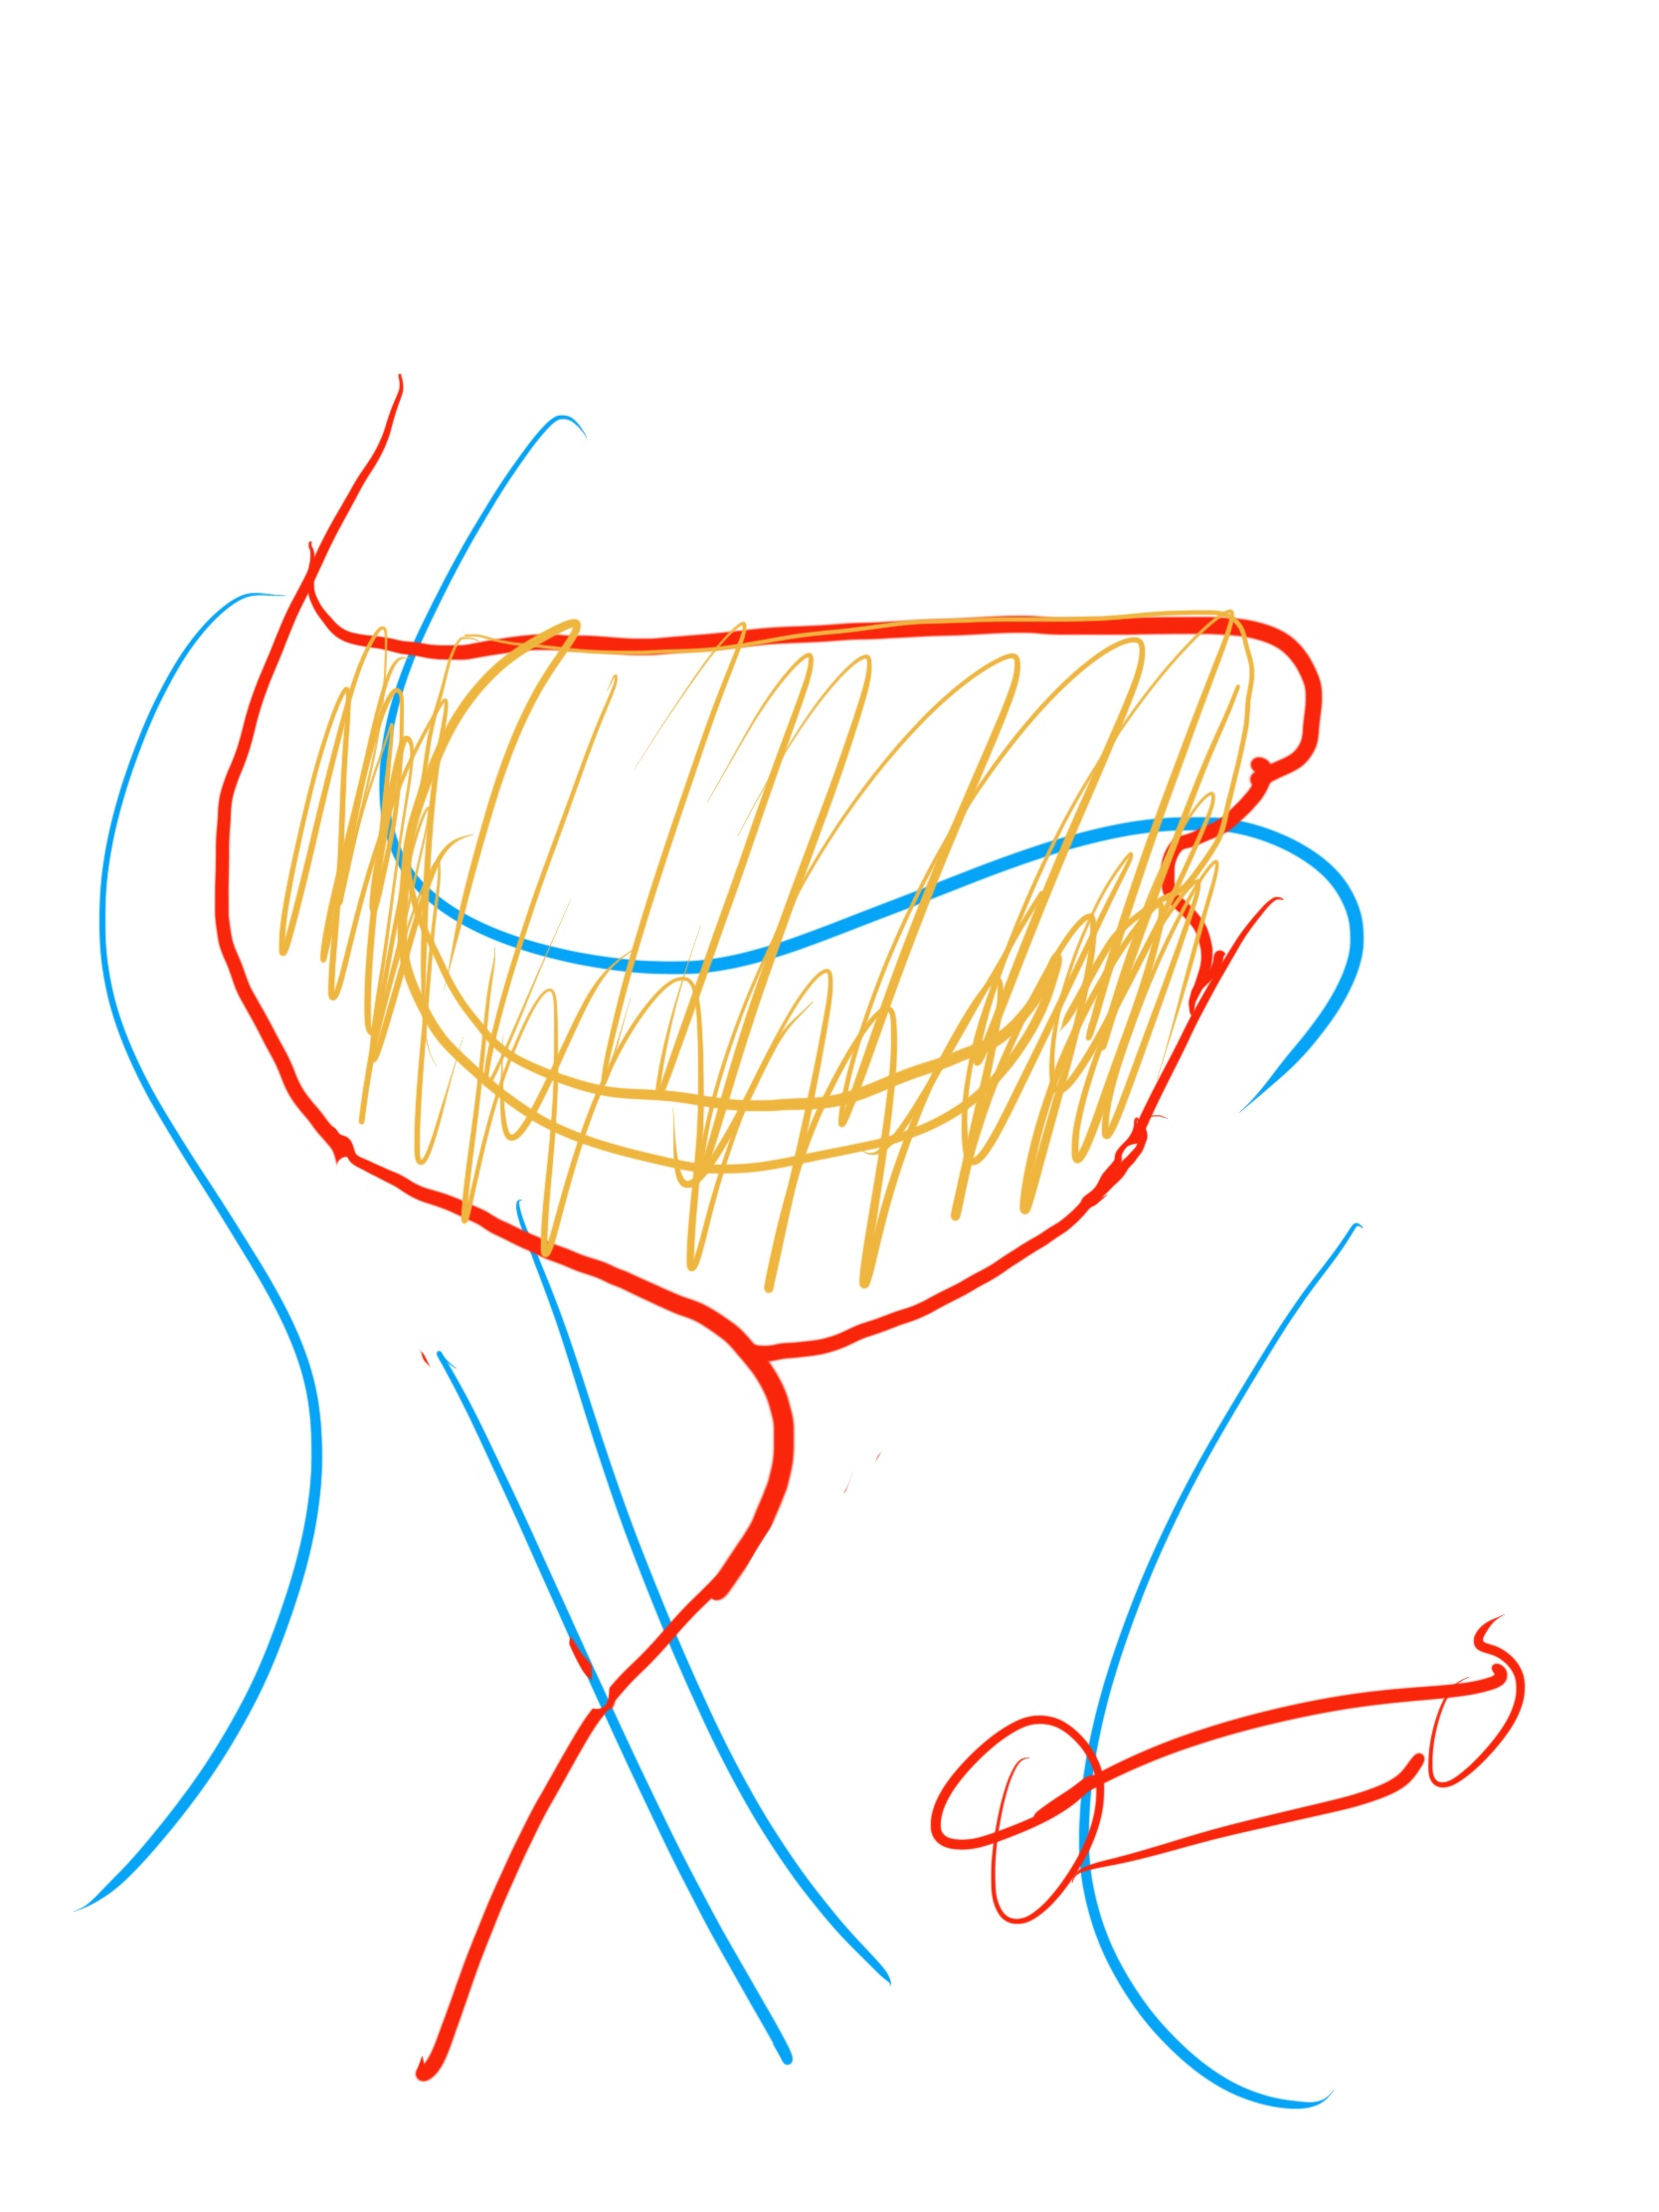
\includegraphics[width=3.5cm]{SOHND_Artwork.jpg}
\end{figure}
%    \2 "The results published~\autocite{Chi2021} and shown here are in part based upon data generated by the TCGA Research Network: \url{https://www.cancer.gov/tcga}."

%\1 We do our best ...
%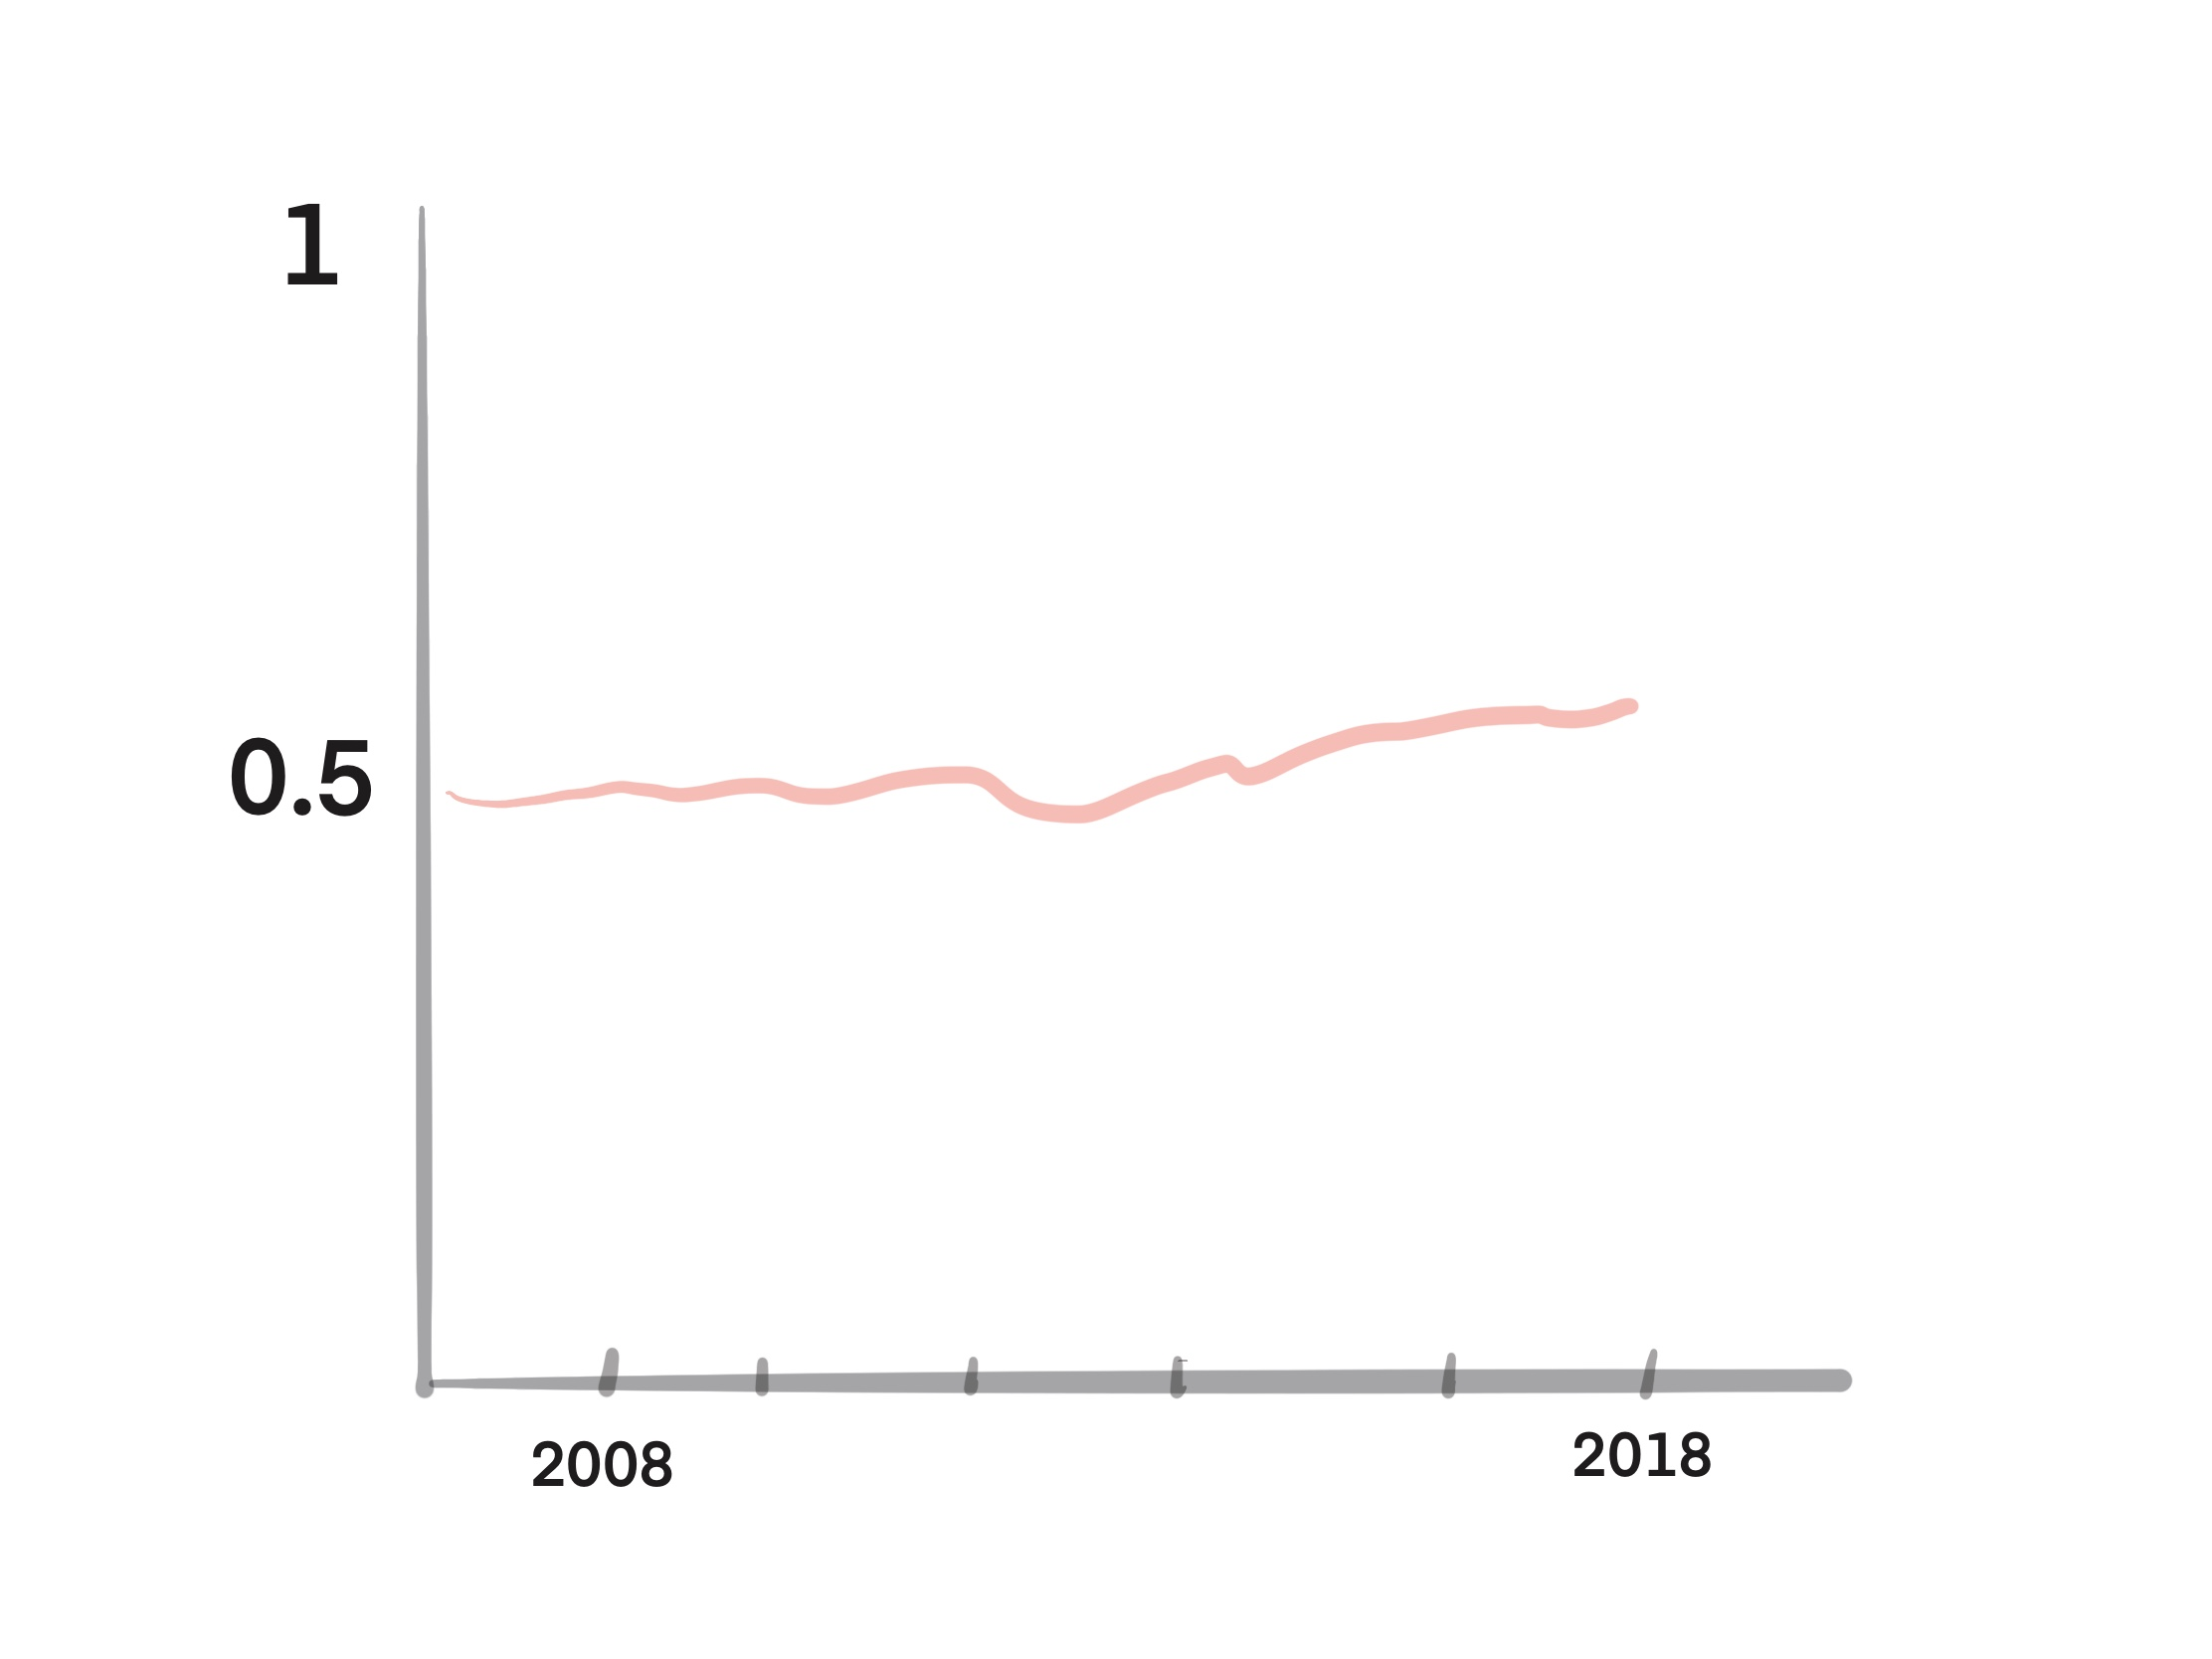
\includegraphics[width=4cm]{stationary_survival_Artwork 2.jpg}

\clearpage
%%
\1 We do
    \2 encourage patients for \hl{correction} of their life style;
    \2 \textcolor{green}{wider excision} (T+N) and better free-flap \textcolor{green}{reconstruction}.
%    \2 to find more useful \textcolor{red}{biomarkers}
\end{outline}




\clearpage

%%%%%%%%%%%
\thispagestyle{headings}
%\markright{Introduction\hfill We do HNSCC therapy \hfill}

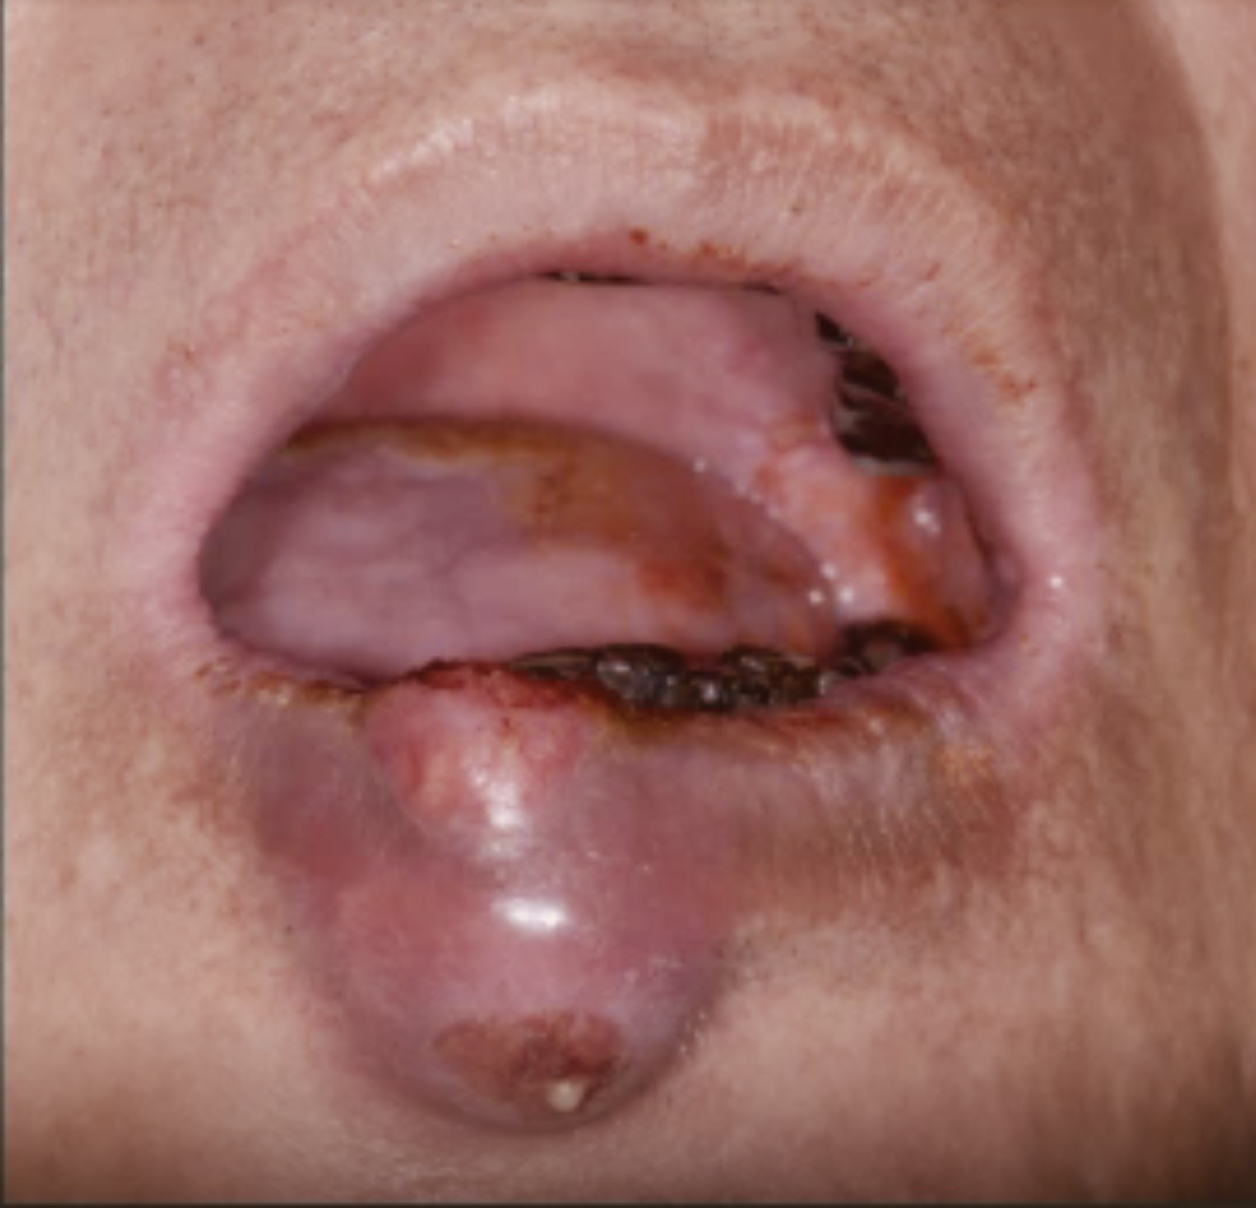
\includegraphics[width=2cm]{IMG_7174.jpg}
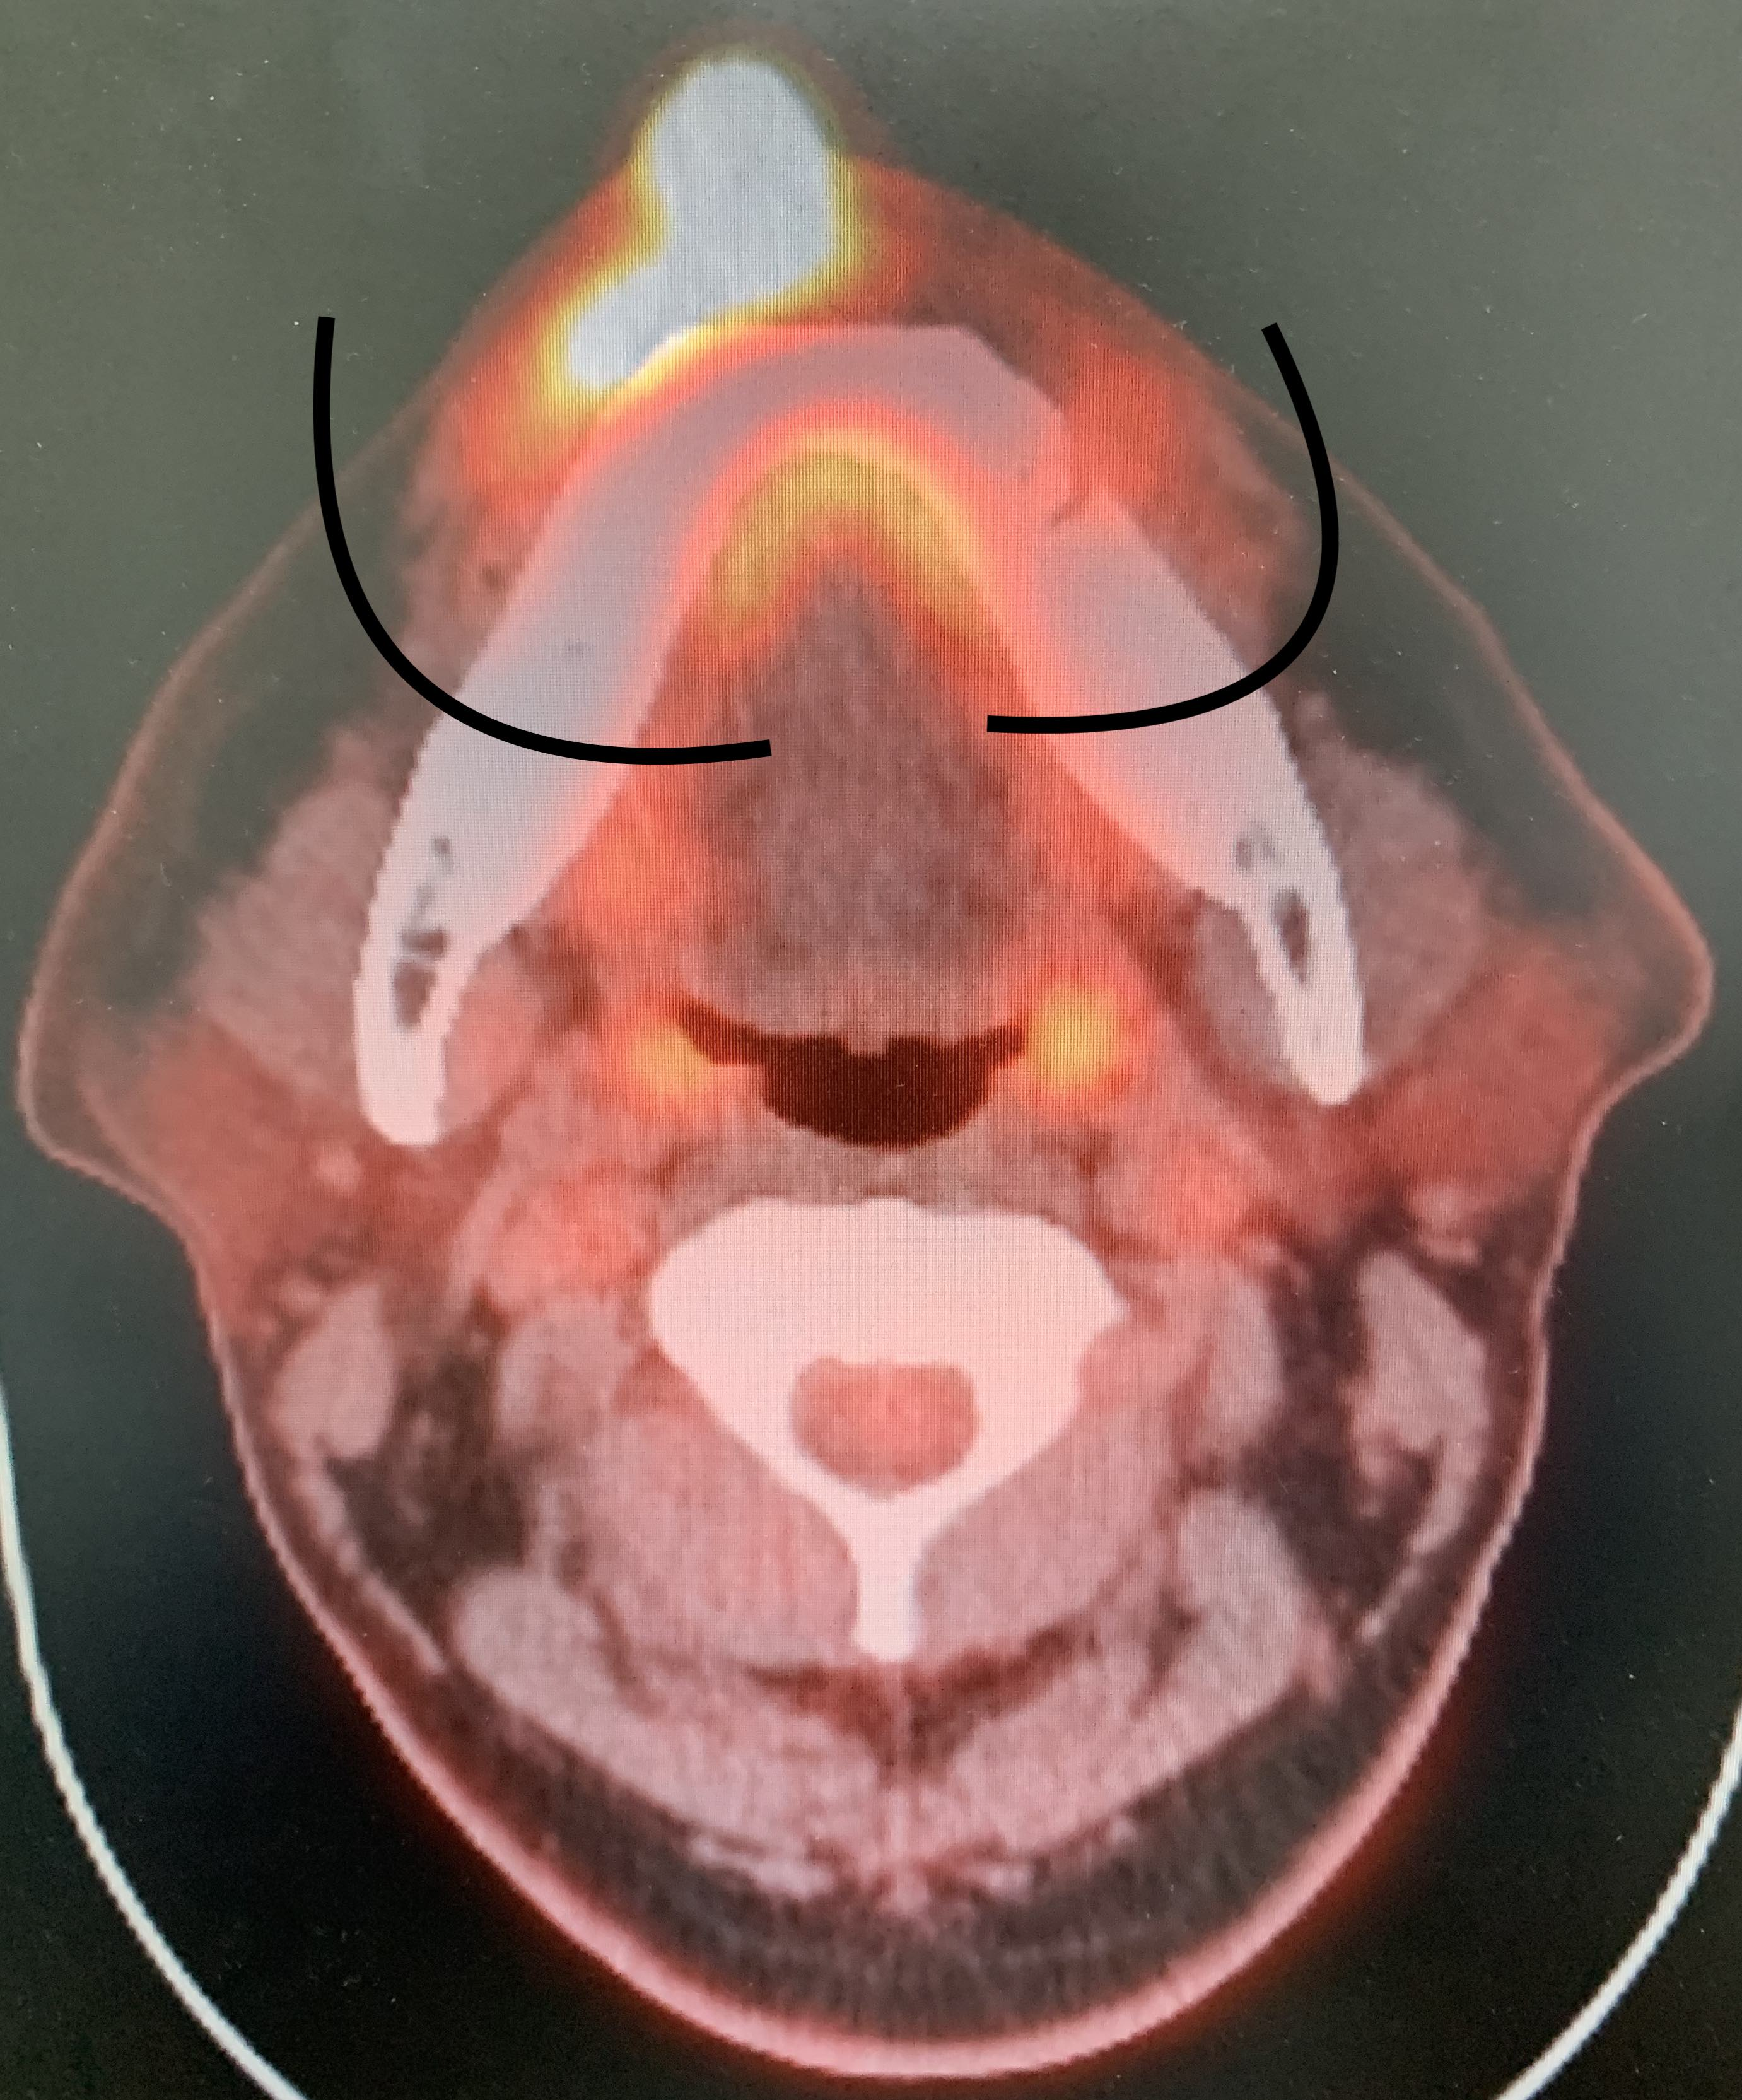
\includegraphics[width=4cm]{IMG_6430.jpg} % PET/CT scan
%\begin{figure}[!h]
%    \centering
%    \caption*{(Image courtesy of Guatacara et al., 2018)}
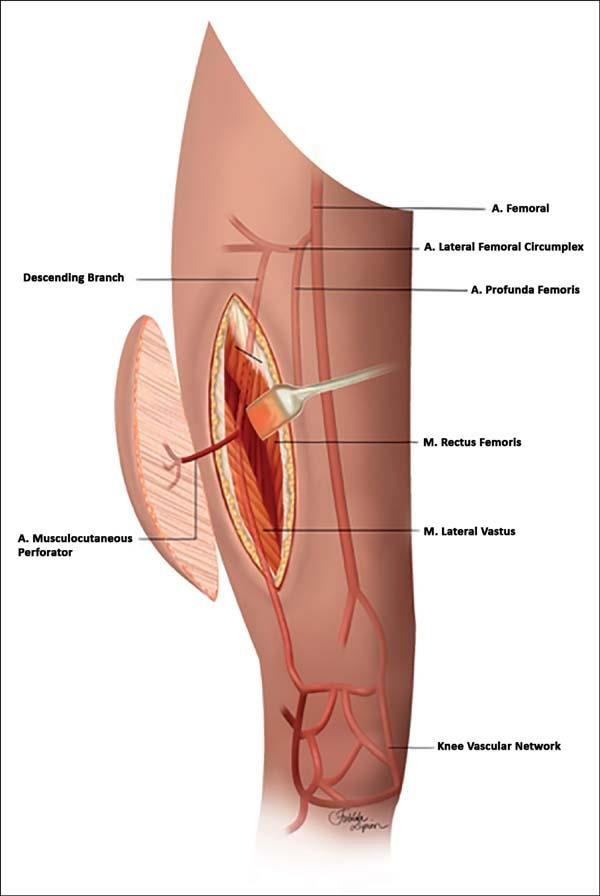
\includegraphics[width=4cm]{Figure-5-Vascular-anatomy-of-ALT-flap-Guatacara-et-al-2018_W640.jpg}\\
\large Wide excision (cut on black line) with selected neck (lymph nodes) dissection\\
\hspace{2cm} 
{\tiny (The illustration courtesy of Guatacara et al., 2018) \par}


% https://www.researchgate.net/publication/337208414_Anterolateral_thigh_versus_radial_forearm_free_flaps_in_reconstruction_of_oral_cavity_malignant_defects/figures?lo=1
%\end{figure}
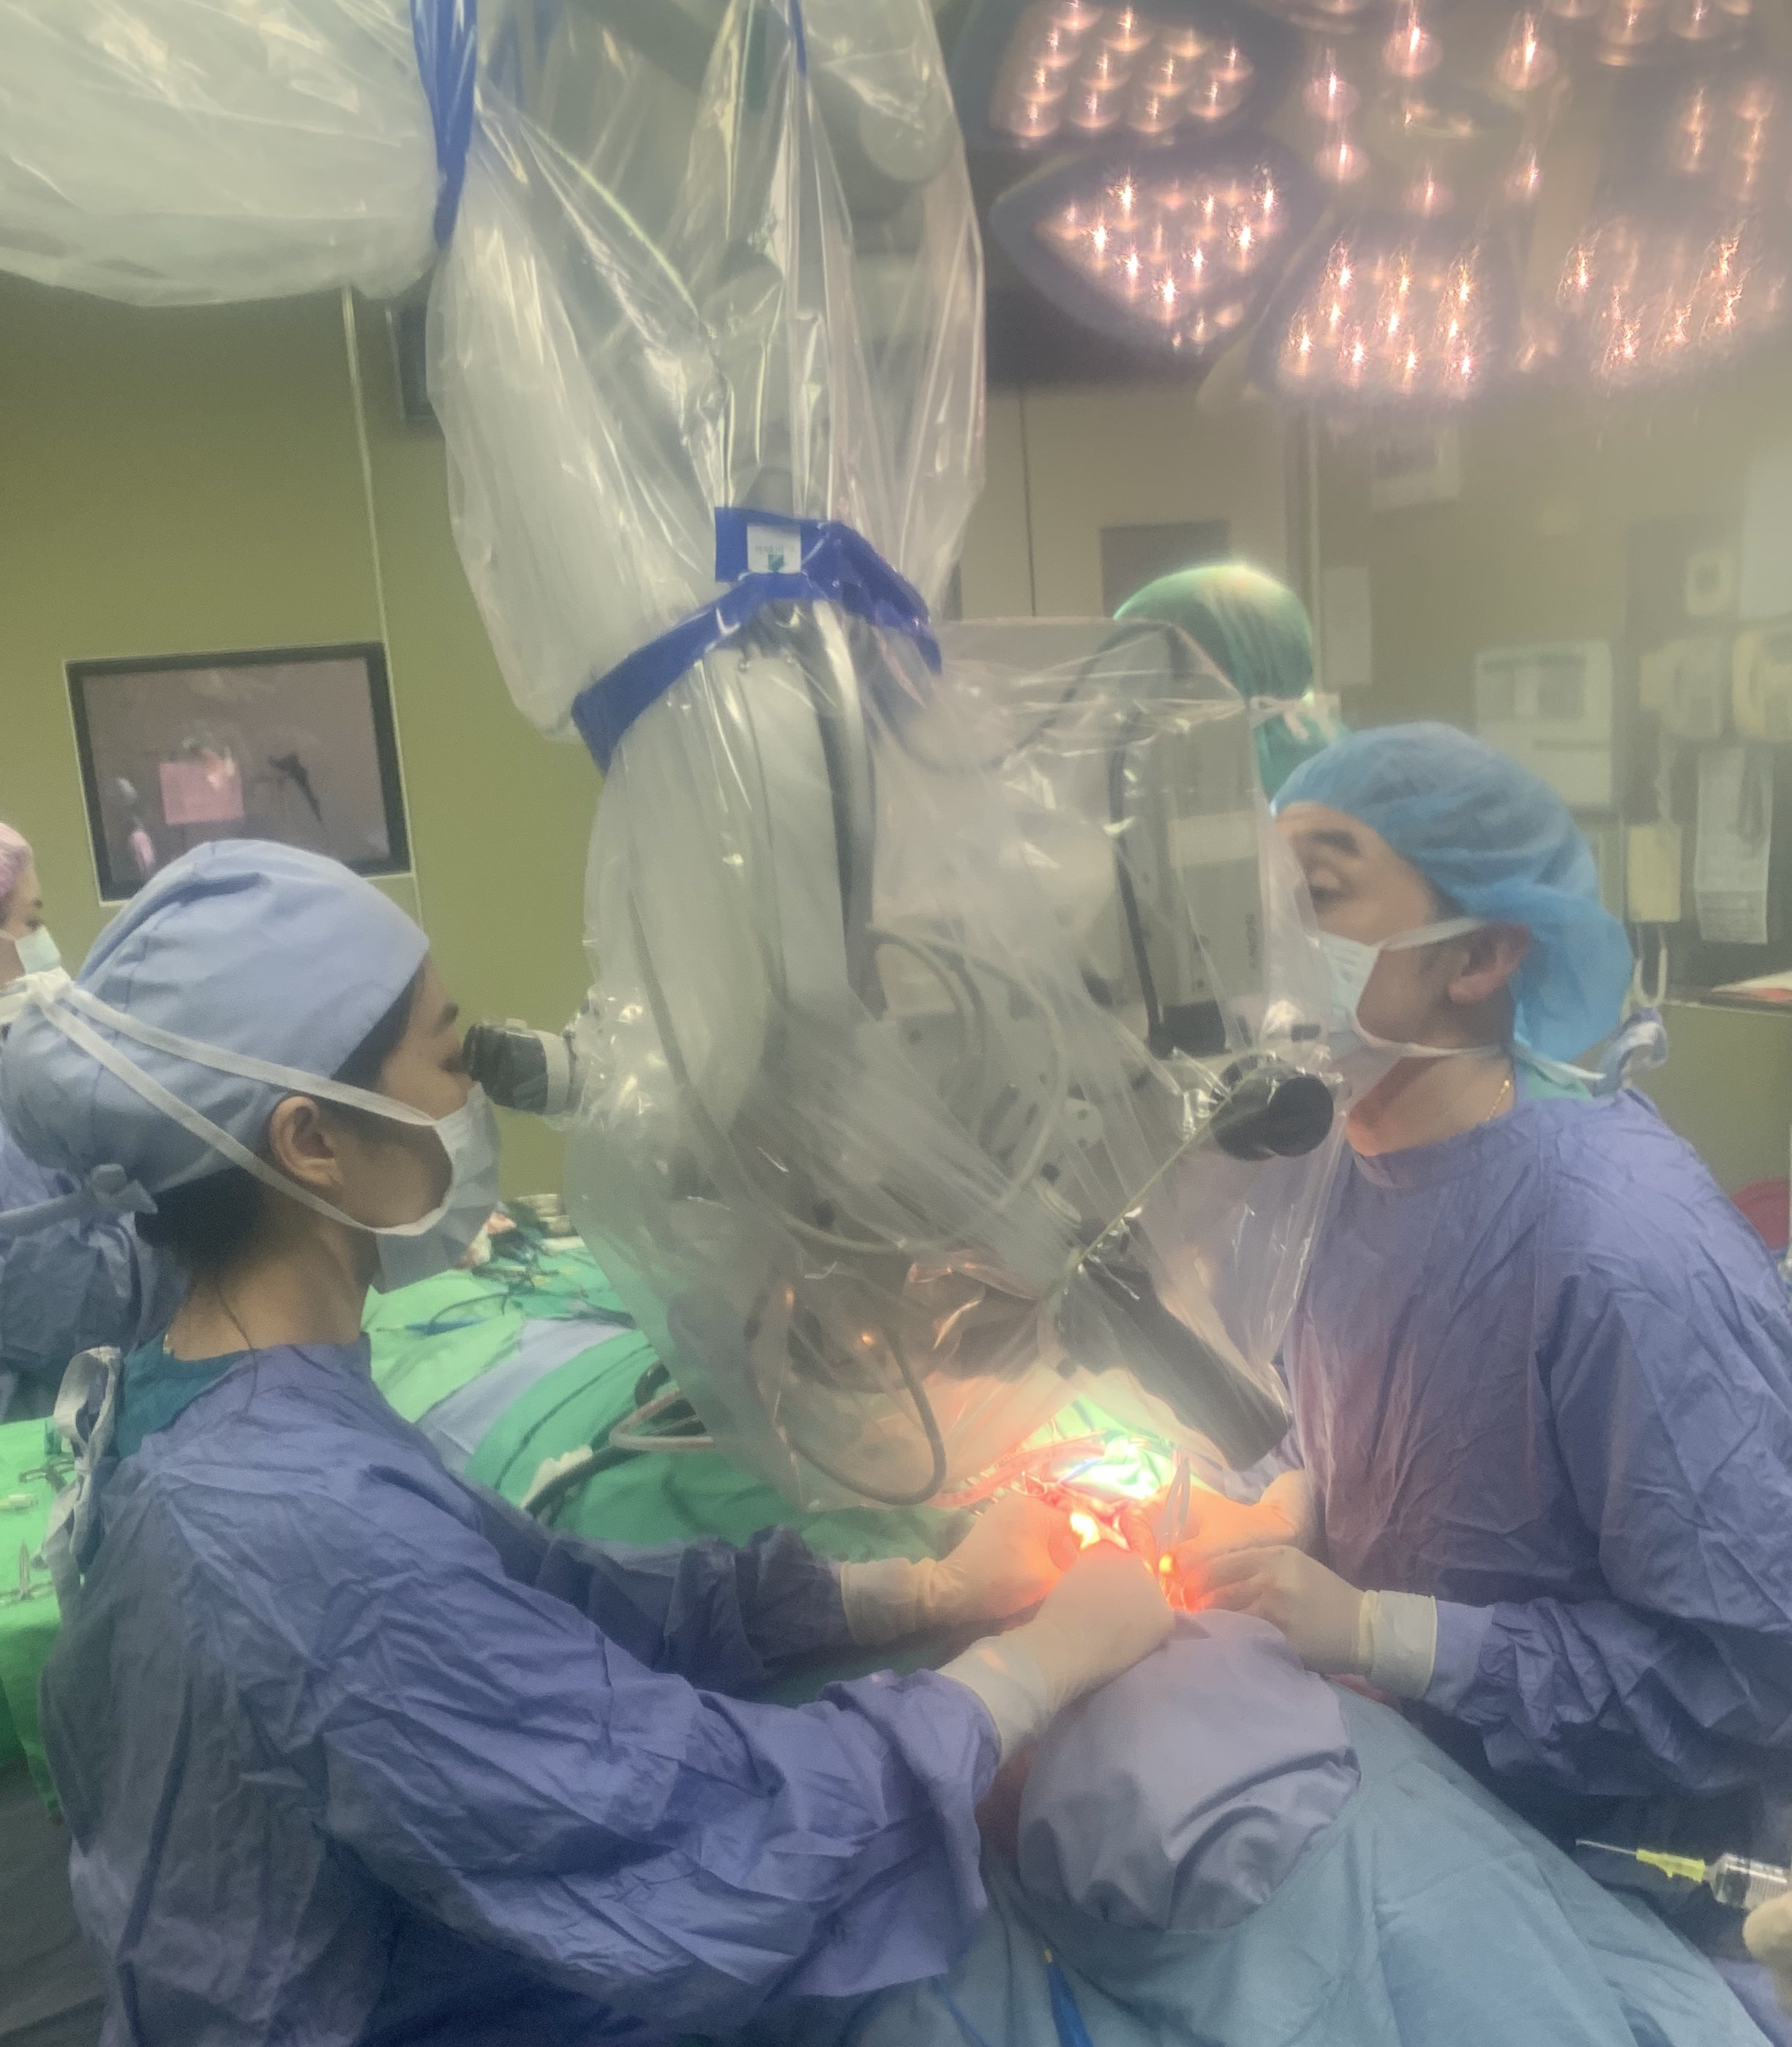
\includegraphics[width=5cm]{IMG_6791.jpg}
\includegraphics[width=6cm]{IMG_6910.jpg}\\
\large Reconstruction with free flap (tissue transfer) under micro-surgery team\\
{\tiny (Photos courtesy of TMU team: Dr. CY Wu and Dr. Evienne Hong on 2021/11/17)}

\clearpage
%% f/u 2009 to 2021 our thinking process: biomarker, screening TCGA, deep learning and holistic
\thispagestyle{headings}
%\markright{Introduction\hfill We do HNSCC research \hfill}

\large Since surgery, we follow patients up closely, and they are always \hl{anxious} about their \hl{recurrence} (so do I).\vspace{5mm}

\begin{outline}
\0 The ways we do for improving our confidence of their prognosis, by
\1 biomarkers discovery from \hl{(A) proteomics} and \hl{(B) transcriptomics} research:
    \2 (A) the in-house HNSCC datasets (in vitro, in vivo)~\parencite{Chi2017};
    \2 (B) the public \acrfull{rnaseq} databases (in silico)~\autocite{Chi2021};
\1 investigation of \hl{surgical margin} (T) and \hl{neck metastasis} (N) by deep learning algorithm (grant proposal);
\1 development of \hl{holistic} cancer care in Taipei Medical University affiliated Hospitals.

\end{outline}
\clearpage



%%
\begin{outline}
\0 Other maxillofacial surgery

\1 alveolar (al-VEE-oh-lar) ridge augmentation
\1 orthognathic (ore-theg-NATH-ick) surgery
    \2 genioplasty (JEE-nee-oh-plas-tee)
\1 cleft lip/palate repair
\end{outline}
\includegraphics[width=4cm]{ridge_augmentation.png}
\includegraphics[width=4cm]{genioplasty.png}
\includegraphics[width=4cm]{cleft.png}

\clearpage

} % end of \comm in section HNSCC


\comm{
%%
\subsection{Oral Surgery Procedures Involved with TMJ Dysfunction}


% - is up text, + is down image
\wrapr{-8mm}{7}{6cm}{-1mm}
{% figure
\includegraphics[width=5.5cm]{MRI.png}
\includegraphics[width=5.5cm]{arthroscope.png}
} % end of figure
{% text
\begin{outline}
\0 disorder of the temporomandibular joint (TMJ)
\1 diagnosis
\2 magnetic resonance imaging (MRI, mæɡ-NET-ik RE-zənəns IMI-dʒiŋ)
\1 treatment
    \2 arthroscope
    \2 arthroplasty (Are-throw-plas-tee)
    \2 arthrotomy (ar-THRAH-toh-me = cutting into a joint)
\end{outline}
} % end of text

\clearpage
} % end of \comm in section HNSCC


%%
\subsection{Surgical Procedures Involved in Dental Implantology}

% - is up text, + is down image
\wrapr{-8mm}{7}{6cm}{-1mm}
{% figure
\includegraphics[width=5.5cm]{ridge_augmentation.png}
\includegraphics[width=3.6cm]{dental_implant.png}
} % end of figure
{% text
\begin{outline}

\1 osseointegrated implants
    \2 endosteal (en-DOSS-tee-ahl = placement within the bone)
    \2 pure titanium: biocompatible with high strength
    \2 abutment (ə-BAT-mənt)
    \2 fixed partial denture (DEN-tʃə = a crown)
\end{outline}
} % end of text

\clearpage
%%
\subsection{Oral Surgery Role in Esthetic Dentistry}


% - is up text, + is down image
\wrapr{-8mm}{7}{6cm}{-1mm}
{% figure
\includegraphics[width=5.5cm]{plastic_face.jpeg}
%\includegraphics[width=3.6cm]{dental_implant.png}
} % end of figure
{% text
\begin{outline}

\1 cleft lip repair
\1 cosmetic alterations
    \2 fixed partial denture
    \2 blepharoplasty (BLEF-er-oh-plas-tee): for eye
    \2 rhinoplasty (RINE-no-plas-tee): for nose
    \2 injectible botox
\end{outline}
} % end of text
\clearpage

%

%%
%%% Chi2017 %%%%%%%%%%%%%%%

%%% Chi2021 %%%%%%%%%%%%%%%


\subsection*{After radiotherapy} 

\subsubsection{Salivary Gland Dysfunction and Radiation Caries}

\subsubsection{osteoradionecrosis of jaw bone}

\thispagestyle{headings}
\markright{Conclusion \hfill Holistic cancer care \hfill}

Holistic (whole) care: to care \hl{spirit}, \hl{emotion}, \hl{the body} of a person, and his \hl{social} relation.

It is the unknown piece of the puzzle in cancer care.\\
%Deep learning and holistic cancer care in the future: Chi2022
\includegraphics[width=4cm]{piece.jpg}
%%%%%%%%%%%%%%%%%%%%
%%%%%% carcinogenesis

%\comm{ % comment it out

\begin{figure}[ht]

\begin{minipage}[c]{0.50\linewidth}
%\floatbox[{\capbeside\thisfloatsetup{capbesideposition={right,center},capbesidewidth=.25\linewidth,capbesidesep=quad}}]{figure}[\FBwidth]
%\centering

\setlength{\unitlength}{.78cm}
\begin{picture}(20, 10)(0,0) %(1,0.55038404)%
%\centering
  \put(0,0){\includegraphics[width=9.0cm]{Figure_5_holisticCare.pdf}}%
  \put(0.4, 9.3){\fontfamily{qcr}\selectfont
  \textbf{[Physician]}}%
  \put(4.0, 9.3){\fontfamily{qcr}\selectfont
  \textbf{[Patient]}}%
  \put(6.0, 7.8){\fontfamily{qcr}\selectfont
  \small OVH }
\end{picture}
%\includegraphics[width=10cm]{Figure_5_holisticCare.pdf}
\end{minipage}
\hfill
\begin{minipage}[c]{0.40\linewidth}
%{\caption{
%The concept of holistic care for \acrshort{hnscc} patients. %MDPI: please confirm if the extra lines and frame need to be deleted.

Carcinogenesis:\\
\hl{The mind--brain--body axis}~\autocite{Hsiao2012}
\small
\begin{outline}
\1 \hl{stress} %ful environment(giant \textcolor{black}{black} arrow) 
will trigger an emotional response in mind
\1 brain releases stress hormones and \hl{inflammation signals} in cells% in response to negative emotions.
\1 %The  body's internal environment (cells) 
altering epigenetic control in \hl{gene regulation} %and mRNA/miRNA expression %of cells
%Over a long time, the tissue/cells will be transformed into dysplasia and then 
\1 Oral verrucous hyperplasia (OVH) -> \hl{transforming} to HNSCC
%\1 carcinogenesis~\autocite{Lutgendorf2010,Powell2013,Iftikhar2021} with help from other known carcinogens
\end{outline}

\end{minipage}

%%%\label{fig:figure5}
\end{figure}
\clearpage

%} % end of \comm
%%%%%%%%%%%%% care
\comm{ % comment it out
\begin{figure}[ht]

\begin{minipage}[c]{0.50\linewidth}
%\floatbox[{\capbeside\thisfloatsetup{capbesideposition={right,center},capbesidewidth=.25\linewidth,capbesidesep=quad}}]{figure}[\FBwidth]
%\centering

\setlength{\unitlength}{.78cm}
\begin{picture}(20, 10)(0,0) %(1,0.55038404)%
%\centering
  \put(0,0){\includegraphics[width=9.0cm]{Figure_5_holisticCare.pdf}}%
  \put(0.4, 9.3){\fontfamily{qcr}\selectfont
  \textbf{[Physician]}}%
  \put(4.0, 9.3){\fontfamily{qcr}\selectfont
  \textbf{[Patient]}}%
  \put(6.0, 7.8){\fontfamily{qcr}\selectfont
  HNSCC}
\end{picture}
%\includegraphics[width=10cm]{Figure_5_holisticCare.pdf}
\end{minipage}
\hfill
\begin{minipage}[c]{0.45\linewidth}
%Holistic cancer care~\autocite{Mehta2019,Iftikhar2021}:

\small
\begin{outline}
\1 to give the \textcolor{green}{physical care}: surgery and/or systemic therapy (drug)
%\1 to support cancer patients' spiritual, emotional, physical, and socioeconomic needs

\1 \textcolor{green}{therapeutic relationship (TR)}~\autocite{Rogers1979}
    \2 the physicians' spiritual properties \hl{(empathy, sympathy, and compassion)} $\longrightarrow$ cancer patients
    \2 $\longrightarrow$ their \hl{self-compassion} $\longrightarrow$ \hl{resilience} $\longrightarrow$ their mind--brain--body axis $\longrightarrow$ the disease~\autocite{Hsiao2012}
\1 to reduce pain, to promote \hl{survival} from cancer

\end{outline}

\end{minipage}

%%%\label{fig:figure5}
\end{figure}
\clearpage
} % end of comment out

%%%%%%%%%%%%%%%%% 2022/02/12
%%SP3
%{\large Subproject Title: Deep Learning Platform of Depression Analysis with Holistic Healthcare to Predict Malignant Transformation of Oral Verrucous Hyperplasia}\\

%\noindent{\rule{\textwidth}{0.4pt}}
    
%This is brief summary of the contents of the exam
	
%This exam contains \numpages\ pages (including this cover page) and \numquestions\ questions.  The total number of  possible points is \numpoints.

% from Tex's Ph.D. dissertation [Chi2022]:
%According to the National Comprehensive Cancer Network (NCCN) guidelines (Version 3.2021~\citep{Pfister2021}), the current treatment of \acrfull{hnscc} should include of surgery alone, radiation therapy alone, or a combination of the two with adjuvant chemotherapy.
%Despite advancements in these therapies, the five-year survival rate for this disease has only marginally improved over the previous decade, and recurrent disease is seen in up to 50\% of all patients~\citep{Forastiere2001,Warnakulasuriya2009}.
%During 2008 to 2018 in Taiwan, the one-year survival rate for this disease among males is from 79.56\% to 81.62\%~(statistics from Cancer Registry of \acrlong{Thpa}, available at \url{https://cris.hpa.gov.tw/pagepub/Home.aspx}, accessed on August 2021).
%The five-year survival rate for this disease among males ranged from 55.13 percent to 56.03 percent between 2009 and 2014.

%Oral verrucous hyperplasia (\acrshort{ovh}) is a premalignant exophytic oral mucosal lesion with a predominantly verrucous or papillary surface; this lesion can subsequently transform into verrucous carcinoma (VC), a well-established warty variant of squamous cell carcinoma (SCC).

%Biomarkers of cancer have been utilized for diagnostic, predictive or prognostic purposes. 
%A predictive marker helps to select which specific treatment benefits a better survival.
%For example, adjuvant radiation therapy should be done after tumor-ablative surgery in positive surgical margin or metastatic lymph node from the neck dissection. %; it  to select a particular treatment over another.
%It guides to determine which further treatment (e.g., ).
%In \acrshort{ovh}, a predictive biomarker gives early alarm of its malignant transformation, which prevents unnecessary biopsy repeatedly.

%A prognostic marker infers the natural history of disease (survival), which is independent on treatment of choice. Gene-expression based biomarker can indicate a need for further treatment, but does not help to determine which treatment. 
	
\comm{ % comment out
	

%%% for figure HE2RNA
\begin{minipage}[c]{0.95\linewidth}
%\smartdiagramset{uniform sequence color=true}
% sequence diagram; flow diagram:horizontal
% 2021
% Figure 5 HE2RNA workflow
\begin{figure}[H]
\centering
%\setcounter{figure}{0}
%\setcounter{diagram}{4}
%\newcounter{diag} % as zero
%\setcounter{diag}{\value{figure}} % for floating environment

%\begin{center}
%\smartdiagram[sequence diagram]{2021/July, Aug, Sep, Oct, Nov, Dec}
\vspace*{30mm}
\smartdiagramset{
    module x sep=3.0cm,
%    module minimum width=3cm,
    text width=2cm,
    back arrow disabled=true,
    border color=none,
    arrow tip=to,
    additions={
additional item bottom color=orange!60!yellow,
   additional item border color=gray,
   additional item shadow=drop shadow,
   additional item offset=0.5cm,
   additional arrow line width=2pt,
   additional arrow tip=to,
   additional arrow color=orange!60!yellow,
    }%,
   %set color list={blue!50!cyan,green!60!lime,orange!50!red,red!80!black},
}

%\smartdiagramset{module x sep=5}
%\smartdiagram[flow diagram:horizontal]{TMU cohort (WSI/EHR), HE2RNA, RNA-Seq}
\smartdiagramadd[flow diagram:horizontal]{
 TMU dataset (WSI), HE2RNA, RNA-Seq (Representation) % module1 2 3
}{
    above of module2/Model (transfer from TCIA) %,
%    below of module3/%Survival Analysis 
} % addition x2
\smartdiagramconnect{to-}{module2/additional-module1}
%\smartdiagramconnect{-to}{module3/additional-module2}

\vspace*{5mm}
\smartdiagramadd[flow diagram:horizontal]{
 TMU dataset (EHR/HRV), \acrshort{rnn}, Survival Analysis
}{}
%\smartdiagramconnect{-to}{module3/module3}
%\begin{tikzpicture}[overlay]  
%\draw[-stealth,line width=1mm,green!40] 
%(module-title3.south) to[out=120,in=-120] (module-title2.north);
%\end{tikzpicture} 

%{
%    above of module2/Model (transfer from TCIA),
%    below of module3/Survival Analysis 
%} % addition x2
%\smartdiagramconnect{to-}{module2/additional-module1}
%\smartdiagramconnect{-to}{module3/additional-module2}
%\vspace*{30mm}
%\smartdiagramset{border color=none, set color list={blue!50!cyan,green!60!lime,orange!50!red,red!80!black}, back arrow disabled=true}

%\smartdiagramset{module x sep=5}
%\smartdiagram[flow diagram:horizontal]{Aim1, Aim2, Aim3}
\end{figure}
\footnotesize 
TCGA: \acrlong{tcga},
TCIA: \acrlong{tcia},
WSI: whole-slide images of pathology,
EHR: \acrlong{ehr}, HRV: \acrlong{hrv},
RNA-Seq: \acrlong{rnaseq},
\acrshort{rnn}: \acrlong{rnn}. 
\end{minipage}
%
%\begin{minipage}[c]{0.45\linewidth}
%\includegraphics[width=14cm]{Figure_HE2RNA.pdf}
%\bcaption{}{} %\captionof{diag} for floating "diag"
%\bcaption{
% ***Workflow of RNA-Seq representation of TMU dataset.
%The deep learning model of HE2RNA, which was trained under TCGA/TCIA \acrshort{hnscc} dataset, could be applied for RNA-Seq prediction of TMU dataset. The representation will be used for subsequent survival analysis.

%} %uncorrected \textit{P} value.}
%\label{fig:HE2RNA}
%\end{minipage}
%\end{center}

%\clearpage

\clearpage


%\vspace{3em}
%\end{minipage}

% make Figure 6
\begin{figure}[hp]
\centering
\includegraphics[width=10cm]{GCNN_survival.pdf}
\bcaption{Overview of the proposed \acrshort{gcnn} for survival analysis}
{\\We suggest that the TMU dataset should collect "holistic features" in electric healthcare records (EHR), which include physical, pathological, psychological data, and spiritual information. Combined with RNA-Seq representation, whole-slide-images pathology and holistic EHR, the \acrfull{gcnn} should extract high-dimensional information for \acrshort{hnscc} survival prediction.}
\label{fig:GCNN}
\end{figure}



\clearpage
\section{Oral management strategies for Chemotherapy and Hematopoietic Stem Cell Transplantation}
% https://www.ncbi.nlm.nih.gov/pmc/articles/PMC9081678/

%%%%
\section{Medication-Related Osteonecrosis of the Jaw (MRONJ)}
\thispagestyle{headings}
\markright{Results \hfill Holistic Cancer Biomarkers \hfill}

\begin{outline}
\1 Current or previous treatment with bone-modifying agents, such as a bisphosphonate, denosumab, or an antiangiogenic.
\1 The presence of an exposed necrotic bone or a bone that can be probed through an intraoral or extraoral fistula in the maxillofacial region and that has persisted for longer than 8 weeks.
\1 No history of radiation therapy to the jaws or obvious metastatic disease to the jaws.

\1 Staging of MRONJ is of importance in the decision-making process on how to manage each of the patients. The staging classification proposed in 2014 by the AAOMS guidelines article established the following staging criteria (updated based on new evidence):

    \2 at risk
    \2 stage zero
    \2 stage 1
    \2 stage 2
    \2 stage 3
\end{outline}
\clearpage

\subsubsection{Prevalence of MRONJ}

\subsubsection{What Are the Drugs That Have Been Reported to Be Associated With MRONJ?}
Antiresorptive and Antiangiogenic Therapy


\subsubsection{Common Signs and Symptoms Associated With MRONJ}

\subsubsection{What Is the Mechanism That Leads to MRONJ?}

\subsubsection{Suggestions of Management Protocols}


%\subsubsection{}
%%%%%%%%%%%%%


\section*{Conclusions} % 5
\thispagestyle{headings}
\markright{Conclusions \hfill Physical care \hfill}

\begin{outline}

\1 The microenvironment of HNSCC, influenced by the mind--brain--body axis~\autocite{Hsiao2012}
    \2 Four \hl{biomarker} candidates---TMSB4X, CAMK2N1, CALML5, and FCGBP---which are all heavily associated with the prognosis of \acrlong{os}~\autocite{Chi2017, Chi2021};
    \2 TMSB4X might promote metastasis of \hl{neck lymph nodes} (N+);

%    \2 further exploration and understanding using \hl{holistic} multi-parametric approaches
%\1 Good using a placebo effect in HNSCC cancer care
%    \2 dorsolateral prefrontal cortex~\autocite{Carlino2011} is the origin of a placebo effect
%    \2 Confidence/trust (i.e., \hl{TR}) might promote healing through a mind--brain--body connection manner
    

\1 A grant proposal (machine learning algorithm---deep learning)
    \2 CAMK2N1 might involved in positive \textcolor{red}{surgical margin};
%        \2 CAMK2N1 has moderate correlation with N+ (Pearson's r = 0.07) :-)
    \2 CAMK2N1 might predict \textcolor{red}{neck metastasis} in clinical N0 neck before surgery;
\1 A grant proposal for validation of CAMK2N1 by \hl{laboratory experiments}.

\end{outline}

%
\clearpage

\thispagestyle{headings}
\markright{Conclusions \hfill Spiritual care \hfill}

\begin{outline}


%\1 More holistic features in HNSCC dataset
\1 The HNSCC dataset must collect those "\hl{holistic features}" for further \hl{holistic biomarker} in personalized medicine, from
    \2 electric healthcare records (EHR);
    \2 A grant proposal: \hl{wearable device} (heart rate variability, HRV) is correlation with patient's emotional stress $\longrightarrow$ \hl{malignant transformation} of oral lesions (e.g., verrucous hyperplasia);
    %患者配戴 HRV 心率手錶,檢測治療期間,追蹤期間(一年),患者的心理壓力指數(HRV 數字越小表示交感神經越亢奮、壓力指數高)。
    \2 spiritual assessment (the meaning of life, hope, love/be loved, forgive/be forgiven, relationship with the Most High).
    %Thus, we suggest that electric healthcare records (EHR) should include physical, pathological, and psychological data, and even more spiritual information. The \acrshort{tcga} might collect those "holistic features"  (\textcolor{green}{green} dashed line) for further study of personalized medicine.
\1 A \hl{professional spiritual caregiver} 
    \2 \hl{Mindfulness meditation} is helpful to cancer patients
%    \2 confess for not taking care of their bodies and spirits in the past (\hl{causality})
%    \2 give sincere thanks for their physical body's hard work
\end{outline}
} % end of comment out

%%%%%%%

\begin{figure}
    \centering
\includegraphics[width=11cm]{family_meeting_Cheung202109.jpg}
\end{figure}

%人俯仰於天地之間
%順從四季氣候變化
%保養正氣陶冶性情
%自我療癒身心靈疾病
%自他不二 心存正念 向內看,解決苦之源
%1.衷心懺悔
%2.真心感謝
%3.誠意祝福
%4.永存善念 慈悲
%5.心無恐懼: 情志養生
%每位醫師都可以成為「創傷知情者」幫助我們身邊的病患,懂他的心靈創傷,讓他有安全感, 才有機會改變疾病的走向
%"每一位患者都有自癒能力, 我們知情之後, 也要逐步讓他本人知情, 看見之後, 在良好的「治療關係」中, 協助他們漸漸找回自己的療癒。(以他們自己的腳步)"
%解說:患者的自癒力就是復原力(resilience),  強調「治療關係」(安全、 信任、 分享權力、 自決) 以及”知情”(暸解過往創傷經驗對自身的影響,進而開始療癒的過程)的重要性。
%%%%%%%%%%%%%%%%%%%%%%%%%%%%%%%%%%%%%%%%%%%%%%%%%%%%%%%%%%%%%%%
%\clearpage
%\thispagestyle{headings}
%\markright{Conclusions \hfill An example of holistic assessment in dental record \hfill}

%\includegraphics[height=6.5cm, width=6.5cm]{Holistic_EHR_TMUH_English.pdf}\hfill
%\includegraphics[height=4.5cm,width=7.5cm]{Holistic_EHR_TMUH_Chinese.pdf}


%\clearpage

%%%%
%\section*{Take Home Message}
%\thispagestyle{headings}
%\markright{Take home message \hfill  \hfill}
%\includegraphics[width=14.5cm]{PCA_CarlRogers.pdf}

\clearpage
%%%%%%%





\section*{Textbook: \\
Contemporary Oral and Maxillofacial Surgery (2019)
}
with 2 citations:
\cite{Harris2022}, \cite{Kawashita2020}, \cite{Migliorati2022}
%Dental Terminology (version 2021)\\
%Chapter 14: Oral and Maxillofacial Surgery}
% references
\thispagestyle{headings} % No slide header and footer
\markright{References}
%\bibliographystyle{unsrt}
%\bibliography{TCGA_margin_cutoff.bib, betel.bib, TMSB4X.bib, pvalueTex.bib}
%*****
%\printbibliography % for biblatex
%\clearpage

%------------------------------
\begin{center}
    

%\includegraphics[width=4.5cm]{qrcode_15880804_DentalTerminologyAmazon.png}
\end{center}
%Or version 2007 in \url{shorturl.at/rsuF7}

\clearpage

%------------------

\thispagestyle{empty} % No slide header and footer

\begin{tikzpicture}[remember picture,overlay] % Background box
  \node [xshift=\paperwidth/2,yshift=\paperheight/2] at (current page.south west)
    [rectangle,fill,inner sep=0pt,minimum width=\paperwidth,minimum height=\paperheight/2.1,top color=myblue,bottom color=myblue]{}; % Change the height of the box, its colors and position on the page here
\end{tikzpicture}
% Text within the box
\begin{flushright}
  \vspace{1.6cm}
  \color{white}\sffamily
  {\bfseries\Huge Thanks for your attention \\Comments and suggestions\par}% Title
  \vspace{0.5cm}
  \normalsize
%  \myauthor\par % Author name
%  \mydate\par % Date
  \myuni\par
  \vfill
\end{flushright}



%李友專
%蕭宏昇
%吳駿翃
%王美娟
%楊欣洲
%王皓青
%張資昊
%----------------------------------------------------------------------------------------
%
\end{document}

%%%%%%%%%%%

\begin{figure}
    \centering
%    \includegraphics{}

\begin{ganttchart}[
    bar label node/.style={text width=5cm,align=right,font=\scriptsize\RaggedLeft,anchor=east},
    x unit=0.8cm,
    y unit title=0.4cm,
    y unit chart=0.6cm, %0.5
    vgrid,
    time slot format=isodate-yearmonth, %compress calendar,
    time slot unit=month,
    title/.append style={draw=none, fill=barblue},
    title label font=\sffamily\bfseries\color{white},
    title label node/.append style={below=-1.6ex},
    title left shift=.05,
    title right shift=-.05,
    title height=1,
    bar/.append style={draw=none, fill=groupblue},
    bar height=.6,
    bar label font=\normalsize\color{black!50},
    group right shift=0,
    group top shift=.6,
    group height=.3,
    group peaks height=.2,
    bar incomplete/.append style={fill=green}
   ]{2021-04}{2022-06}
   
   \gantttitlecalendar{year, month}\\ %=name
   \ganttbar[
    progress=100,
    bar progress label font=\small\color{barblue},
    bar progress label node/.append style={right=4pt},
    bar label font=\normalsize\color{barblue},
    name=pp
   ]{Preliminary Biomarker Discovery}{2021-04}{2021-06} \\ % name=pp
   
\ganttset{progress label text={}, link/.style={black, -to}}
% aim1
\ganttgroup{Aim 1}{2021-07}{2021-12} \\
\ganttbar[progress=10, name=T1A]{Process of pathology images}{2021-07}{2021-10} \\
\ganttlinkedbar[progress=0, name=T1B]{Training deep learning model (CNN)}{2021-10}{2021-12} \\

% aim2
\ganttgroup{Aim 2}{2021-07}{2021-12} \\
\ganttbar[progress=2, name=T2A]{\cntext{Biobank specimen linking to EHR data(*)}}{2021-07}{2021-10} \\ % 因Covid-19,臨床研究資料庫獨立作業區2021.05.19暫停服務

\ganttnewline
\ganttlinkedbar[progress=0, name=T2B]{Development of source code (RNN)}{2021-10}{2021-12} \\


\ganttnewline
% aim3
\ganttgroup{Aim 3}{2021-09}{2022-06} \\
  \ganttbar[progress=0, name=T3A]{Development of GCNN $\&$ survival/validation}{2021-09}{2022-06}
  \ganttnewline
%\ganttgroup{Aim 4}{2021-12}{2022-06} \\ %[group top shift =2] to avoid vertically overlap of bars
%  \ganttbar[progress=0]{Analysis of Experimental Data $\&$ Validation}{2021-12}{2022-06}
  % , bar top shift =1.8
  \ganttset{link/.style={green}}
  \ganttlink[link mid=.4]{pp}{T1A}
  \ganttlink[link mid=.159]{pp}{T2A}
  
  \ganttset{link/.style={black}}
  \ganttlink[link mid=.4]{T1B}{T3A}
  \ganttlink[link mid=.159]{T2B}{T3A}
\end{ganttchart}

    \caption{\cntext{Progress}
    \cntext{(*For COVID-19 pandemic in Taiwan, the data workstation is suspended since 2021.05.19)}}
    \label{fig:gantt}
\end{figure}

\clearpage


%%%%
報告親愛的老師,晚安

1)謝謝老師,百忙之中能參加祁力行的口試 (日期時間:2022/01/12 11:00-12:00, Wednesday);
2)地點(***已變更,不在吳興街),改為「台北市大安區基隆路二段172-1號15樓討論室A」(這是北醫大安校區)。
3)敬請老師填寫「校園訪客登記:數位訪客證」存在手機中即可,
https://glbsys.tmu.edu.tw/guestsign/Apply.aspx
洽公單位請填寫:醫學資訊研究所

4)力行的論文是以口腔癌的治療為骨幹,嵌入 Chi2017 及 Chi2021 兩篇文章,融合改寫、加上deep learning與全人口腔癌照護的概念,總集而成。
博士論文初稿:https://drive.google.com/file/d/1C5iNhcdUzL1LnRiHZ5ZF8LAhZaPMamMB/view?usp=drivesdk

以下為簡介:
Chi2017> 由口腔癌病理檢體,MS mass spectrometry 打碎飛出來的蛋白質片段,來找出生物標記 biomarker (看看什麼基因、蛋白質表現多的,和癌症病患的存活率有關)
發表的文章 https://www.nature.com/articles/s41598-017-09539-w

Chi2021> 則是由口腔癌病理檢體,NGS 基因定序,來找出生物標記 biomarker (看看什麼基因、蛋白質表現多的,和癌症病患的存活率有關)
發表的文章 https://www.mdpi.com/2075-4426/11/8/782/htm;另有video 簡介(十分鐘)
https://encyclopedia.pub/16116

以上報告 麻煩老師了
下週見,謝謝老師
力行敬上
% spared code

%------------------------------------------------

%pstricks

\begin{pspicture}(2008, 0)(2018,100)
\psset{unit=.75cm}
\psaxes[labelFontSize=\scriptstyle]{<->}%
%  (0,0)(2008,0)(2018,100)[$x$-axis,-90][$y$-axis,180]
  \psline[linewidth=1.5pt,
  linecolor=red](2009,55)(2017,57)
\end{pspicture}

\section*{x Verbatim}

How to include a theorem in this presentation:
\begin{verbatim}
\mybox{0.8\textwidth}{
\begin{theorem}[Murphy (1949)]
Anything that can go wrong, will go wrong.
\end{theorem}
}
\end{verbatim}

\clearpage

%------------------------------------------------



\subsection*{Figure}

%\clearfloatsetup{figure}
%\floatsetup[figure]{style=no,capposition=beside,capbesideposition={center,inside},capbesideframe=yes,facing=yes}

\begin{figure}[ht]
\floatbox[{\capbeside\thisfloatsetup{capbesideposition={right,center},capbesidewidth=.35\linewidth,capbesidesep=quad}}]{figure}[\FBwidth]
{\captionsetup{labelformat=empty} \caption{\texttt{capbesidesep=quad}. I want to thank Sonia. The caption can contain any text but needs to describe the image with enough detail for a reader to completely understand the image.}}
{\includegraphics[width=0.6\textwidth]{placeholder.jpg}}
\end{figure}
%\includegraphics[width=9cm]{placeholder}

%\sidecaptionvpos{c}
%\caption{I want to thank Sonia.}
%\end{captionbeside}


\clearpage

%------------------------------------------------

